% ========================================= TEMPLATE INFO ========================================
%
% Author:       P4ntomime
% Version:      1.0.0
% Last updated: 2024-02-18
% Brief:        A LaTeX template for summaries. See README.md for more information.
% 
% ================================================================================================
\documentclass[8pt, a4paper, twoside]{extarticle}
% Font size:    8pt
% Paper size:   A4
% style:        twoside (needed, so odd and even pages have different margins)
% orientation:  portrait. (use 'landscape' for landscape orientation)


% ========================================= DOCUMENT INFO =========================================
\def\title{Signale und Systeme 1}           					% title
\def\shorttitle{SigSys1} 										% short title (displayed as PDF title)
\def\dozent{Prof. Dr. Heinz Mathis}         					% lecturer
\def\semester{HS 2026}     										% semester
\def\author{Simone Stitz, Mirko Ratti}        					% author(s)
\def\repo{https://gitlab.com/sstitz/signale-und-systeme-1}      % repository link
\def\version{3.0.\today}    									% version
\def\pagelimit{20}           									% page limit -> causes pages after limit to be red
\def\titleoption{normal}   										% options: compact, normal
\def\enableToC{true}

% ================================= PACKAGES, SETUP AND COMMANDS ==================================
% =========================================== PACKAGES ============================================
\usepackage[utf8]{inputenc}         % input encoding: UTF-8
\usepackage[T1]{fontenc}            % font encoding: T1
\usepackage{textcomp}               % additional symbols
\usepackage{times}                  % times new roman font
\usepackage{inconsolata}            % inconsolata font for listings
\usepackage[main=ngerman]{babel}    % set main language to german


\usepackage{multicol}               % provides multicols environment
\usepackage{multirow}               % provides multirows environment
\usepackage{geometry}               % set page layout


\usepackage{enumitem}               % list customization
\usepackage{outlines}               % easy nested lists
\usepackage{tabularx}               % some nicer tables with X columns
% \usepackage{tabu}                 % DISABLED: unmaintained/slow, not referenced by any
                                     % custom command here; re-enable only if your
                                     % own documents actually use \tabu / \tabuline etc.
\usepackage{hhline}                 % double lines in tables
\usepackage{booktabs}               % thick and thin lines in tables
\usepackage{boldline}               % bold (vertical) lines in tables


\usepackage{amsmath}                % math symbols
\usepackage{amssymb}                % more math symbols
\usepackage{mathtools}              % more math tools needed for pmatrix modification
\usepackage{mhsetup}                % needed to modify pmatrix environment
% \usepackage{txfonts}              % Deprecated: Times math font
\usepackage{newtxtext}              % New math fonts
\usepackage[libertine]{newtxmath}
\let\laplace\relax
\let\Laplace\relax
\usepackage[squaren]{SIunits}       % SI-units
\usepackage{bm}                     % bold math symbols
\usepackage{trfsigns}             % Deprecated: needed from txfonts for "Laplace" symbol (Korrespondenz)
\usepackage{mathrsfs}               % needed for Fourier transform "F"


\usepackage{graphicx}               % include graphics
\usepackage{graphbox}               % needed for aligning images in multicol environment
\usepackage{scalerel}               % scale any objects
\usepackage{anyfontsize}            % set any font size
\usepackage[table]{xcolor}          % needed for colors


\usepackage{tcolorbox}              % colored boxes
\usepackage[outline]{contour}       % contour for text (used in custom underline command)
\usepackage[normalem]{ulem}         % custom underline (used in custom underline command)


\usepackage{tikz}                   % needed for TikZ drawings
\usepackage{pgfplots}               % Draw nice plots


\usepackage{listings}               % for nicer code display
% to use nodes inside listing see: https://texample.net/tikz/examples/tikz-listings/


\usepackage{hyperref}               % clickable links
\usepackage{qrcode}                 % QR code generation (also clickable)


\usepackage{ifthen}                 % if-then-else commands
\usepackage{calc}                   % simple arithmetic in LaTeX commands


\usepackage{draftwatermark}         % watermark on pages after a certain limit
\usepackage{fancyhdr}               % custom header and footer
\usepackage[explicit]{titlesec}     % custom section titles


\usepackage{datetime2}              % custom date format for versioning


% ========================================== BASIC SETUP ==========================================

% --------------------------------------- DOCUMENT SETTINGS ---------------------------------------
\hypersetup{hidelinks,
% set pdf metadata
            pdfauthor={\author},
            pdftitle={\shorttitle},
            pdfsubject={\title\ \semester},
            pdfkeywords={Gahn go lerne!!}}

% set style for URLs
\urlstyle{same} % sets url font to the same as the preceeding text

% set page layout
\geometry{left=3mm, 
          right=3mm, 
          top=3mm, 
          bottom=6mm, 
          headheight=0mm, 
          headsep=0mm, 
          footskip=4mm,
        %   showframe,
          }

\setlength{\columnsep}{1.5mm}       % distance between columns
\setlength{\columnseprule}{0.1pt}   % thickness of column separation line
\setlength{\parindent}{0pt}         % no paragraph indentation

\setcounter{tocdepth}{2}            % only display sections and subsections in toc
% \setcounter{secnumdepth}{0}       % uncomment to disable section numbering

\DeclareMathSizes{8}{8}{6}{5}       % set math font sizes for 8pt document


% --------------------------------------- COLOR DEFINITIONS ---------------------------------------
\definecolor{sectioncolor}{HTML}{2eebbf}
\definecolor{subsectioncolor}{HTML}{abf7e5}
\definecolor{sectextcol}{HTML}{000000}
\definecolor{subsectextcol}{HTML}{000000}

\definecolor{backcolour}{HTML}{f5f5f0} % background color for highlighted text

% TODO: define color palette
% color palette: https://colorkit.co/color-palette-generator/FF8552-9e22bd-404E7C-C32E15-225A28/
\definecolor{green}{HTML}{1af430}
\definecolor{red}{HTML}{f90d09}
\definecolor{blue}{HTML}{093ce5}
\definecolor{orange}{HTML}{f7730e}
\definecolor{violet}{HTML}{a516c9}

% colors for listings (code)
\definecolor{commentcolour}{HTML}{6a9955}
\definecolor{keywordcolour}{HTML}{7f0055}
\definecolor{stringcolour}{HTML}{9e22bd}
\definecolor{numbercolour}{HTML}{808080}


% ----------------------------------- LIST AND TABULAR SETTINGS -----------------------------------
\setlist[enumerate]{%
    labelindent=0pt,                                % no indentation for labels
    labelwidth = \widthof{\ref{enum-\EnumitemId}},  % set label width to widest label
    label=\bfseries\arabic*.,                       % label style bold arabic numerals (1., 2., ...)
    itemindent=1ex,                                 % separation between label and item text
    leftmargin=!,                                   % automatically calculate left margin
    after=\label{enum-\EnumitemId}}                 % set label for referencing in labelwidth

\setlist[itemize]{leftmargin=1.5em}                 % left margin for itemize: 1.5em
\setlist[description]{leftmargin=2ex}               % left margin for description: 2ex
\setlist{nosep}                                     % no vertical spacing between list items

\renewcommand{\arraystretch}{1}                     % stretch table rows

\setcounter{MaxMatrixCols}{32}                      % increase max columns in matrix environments

% ----------------------------------- TIKZ & PGF-PLOTS SETTINGS -----------------------------------
\usetikzlibrary{arrows}
\usetikzlibrary{arrows.meta}
\usetikzlibrary{bending}
\usetikzlibrary{decorations.pathreplacing}
\usetikzlibrary{angles}
\usetikzlibrary{tikzmark}
\usetikzlibrary{petri}
\usetikzlibrary{positioning}
\usetikzlibrary{shapes}
\usetikzlibrary{calc}

\pgfplotsset{compat=1.18}

% ------------------------------------ OTHER PACKAGE SETTINGS -------------------------------------

% define and set new date style for versioning as YYYYMMDD
\DTMnewdatestyle{vnumdate}{%
    \renewcommand{\DTMdisplaydate}[4]{\number##1\DTMtwodigits{##2}\DTMtwodigits{##3}}%
    \renewcommand{\DTMDisplaydate}{\DTMdisplaydate}%
}
\DTMsetdatestyle{vnumdate}


% setup for ulem and contour packages
\renewcommand{\ULdepth}{1.75pt} % set underline depth
\contourlength{0.7pt}           % set contour length


% ====================================== SETUP AND COMMANDS =======================================

% custom font size for paragraph titles
\newcommand{\semilarge}{\fontsize{9}{8}\selectfont} % new font size \semilarge (9pt)

\ExplSyntaxOn
% custom underline command for exclusions on lowercase letters such as g, j, p, q, y
\newrobustcmd{\myul}[1]{%
    \if_mode_math:
        \text{%
            \uline{\phantom{$#1$}}%
            \llap{\contour{white}{$#1$}}%
        }
    \else:
        \uline{\phantom{#1}}%
        \llap{\contour{white}{#1}}%
    \fi:
}

\renewrobustcmd{\underline}[1]{%
    \if_mode_math:
        \text{%
            \uline{\phantom{$#1$}}%
            \llap{\contour{white}{$#1$}}%
        }
    \else:
        \uline{\phantom{#1}}%
        \llap{\contour{white}{#1}}%
    \fi:
}
\ExplSyntaxOff


% setup header and footer
\pagestyle{fancy}
\fancyhf{}                          % clear all header and footer fields
\renewcommand{\headrulewidth}{0pt}  % remove header rule
\renewcommand{\footrulewidth}{0pt}  % remove footer rule
\fancyfoot[C]{\thepage}             % page number in center of footer


% --------------------------------------- TITLE FORMATTING ----------------------------------------

\titleclass{\part}{straight}

% part formatting
\titleformat{\part}
            {\huge\bfseries}
            {\thepart}
            {1em}
            {#1}

\titlespacing{\part}
             {0.6ex}
             {1ex}
             {1ex}

% lightweight colored heading box (replaces a \tikz{\node[...]} per heading:
% same visual result -- colored background, fixed height, left aligned text --
% but without going through the pgf/TikZ machinery on every single heading,
% which is by far the most called piece of TikZ code in a large document.
\newcommand{\headingbgbox}[3]{% #1=fill color, #2=text color, #3=content
    \begingroup
    \setlength{\fboxsep}{2pt}%
    \colorbox{#1}{%
        \textcolor{#2}{%
            \parbox[c][3.8mm][c]{\dimexpr\columnwidth-4pt\relax}{\raggedright#3}%
        }%
    }%
    \endgroup
}

% section formatting
\titleformat{\section}
            % {\fontsize{9}{8}\selectfont\bfseries}
            {\Large\bfseries}
            {}
            {0mm}
            {\headingbgbox{sectioncolor}{sectextcol}{\thesection\ #1}}

\titleformat{numberless, name=\section}
            % {\fontsize{9}{8}\selectfont\bfseries}
            {\Large\bfseries}
            {}
            {0mm}
            {\headingbgbox{sectioncolor}{sectextcol}{#1}}

\titlespacing{\section}
             {0mm}
             {.2ex}
             {.2ex}


% subsection formatting
\titleformat{\subsection}
            {\large\bfseries}
            {}
            {0mm}
            {\phantomsection\headingbgbox{subsectioncolor}{subsectextcol}{\thesubsection\ #1}}

\titleformat{numberless, name=\subsection}
            {\large\bfseries}
            {}
            {0mm}
            {\phantomsection\headingbgbox{subsectioncolor}{subsectextcol}{#1}}

\titlespacing{\subsection}
             {0mm}
             {1ex}
             {.2ex}


% subsubsection formatting
\titleformat{\subsubsection}
            {\large\bfseries}
            {\myul{\thesubsubsection\ }}
            {0mm}
            {\phantomsection{}\myul{#1}}

\titlespacing{\subsubsection}
             {0mm}
             {1ex}
             {1ex}


% paragraph formatting
\titleformat{\paragraph}[runin]
            {\semilarge\bfseries}
            {}
            {0mm}
            {#1\normalfont :\;}

\titlespacing{\paragraph}
             {0mm}
             {0ex}
             {0.1ex}


% new alias for paragraph '\para' (shorter than \paragraph)
\let\para\paragraph%

% custom command for examples
\newcommand{\example}[1]{\subsubsection*{Beispiel: #1}}


% ----------------------------------- CUSTOM TABULAR SPECIFIERS -----------------------------------

% centered fixed width column type
\newcolumntype{P}[1]{>{\centering\arraybackslash}p{#1}}

 % centered variable width column type
\newcolumntype{C}{>{\centering\arraybackslash}X}

% centered math column type
\newcolumntype{M}{>{$}c<{$}}


% inline tikz node for later referencing
\newcommand{\tikznode}[2]{% from https://tex.stackexchange.com/a/402466/121799
	\ifmmode%
	\tikz[remember picture,baseline= (#1.base),inner sep=0pt] \node(#1){$#2$};
	\else
	\tikz[remember picture,baseline= (#1.base),inner sep=0pt] \node(#1){#2};
	\fi}


% custom inline tcolorbox
\newtcbox{\mybox}
            [1]
            [backcolour]
            {on line,
            arc=0pt,
            outer arc=0pt,
            colback=#1,
            colframe=#1,
            boxsep=0pt,
            left=1pt,
            right=1pt,
            top=1pt,
            bottom=1pt,
            boxrule=0pt}


\makeatletter

% ------------------------------- SECTIONING COMMANDS CUSTOMIZATION -------------------------------

% section: add optional argument to command for script page numbers
\let\old@sec\section%
\RenewDocumentCommand{\section}{somg}{%
    \IfBooleanTF{#1}{
        \IfNoValueTF{#2}{
            \IfNoValueTF{#4}{
                \old@sec*{#3}
            }{
                \old@sec*{#3 {\small(S. #4)}}
            }
        }{
            \IfNoValueTF{#4}{
                \old@sec*[#2]{#3}
            }{
                \old@sec*[#2]{#3 {\small(S. #4)}}
            }
        }%
    }{
        \IfNoValueTF{#2}{
            \IfNoValueTF{#4}{
                \old@sec{#3}
            }{
                \old@sec{#3 {\small(S. #4)}}
            }
        }{
            \IfNoValueTF{#4}{
                \old@sec[#2]{#3}
            }{
                \old@sec[#2]{#3 {\small(S. #4)}}
            }
        }%
    }
}


% subsection: add optional argument to command for script page numbers
\let\old@subsec\subsection%
\RenewDocumentCommand{\subsection}{somg}{%
    \IfBooleanTF{#1}{
        \IfNoValueTF{#2}{
            \IfNoValueTF{#4}{
                \old@subsec*{#3}
            }{
                \old@subsec*{#3 {\small(S. #4)}}
            }
        }{
            \IfNoValueTF{#4}{
                \old@subsec*[#2]{#3}
            }{
                \old@subsec*[#2]{#3 {\small(S. #4)}}
            }
        }%
    }{
        \IfNoValueTF{#2}{
            \IfNoValueTF{#4}{
                \old@subsec{#3}
            }{
                \old@subsec{#3 {\small(S. #4)}}
            }
        }{
            \IfNoValueTF{#4}{
                \old@subsec[#2]{#3}
            }{
                \old@subsec[#2]{#3 {\small(S. #4)}}
            }
        }%
    }
}


% subsubsection: add optional argument to command for script page numbers
\let\old@subsubsec\subsubsection%
\RenewDocumentCommand{\subsubsection}{somg}{%
    \IfBooleanTF{#1}{
        \IfNoValueTF{#2}{
            \IfNoValueTF{#4}{
                \old@subsubsec*{#3}
            }{
                \old@subsubsec*{#3 {\small(S. #4)}}
            }
        }{
            \IfNoValueTF{#4}{
                \old@subsubsec*[#2]{#3}
            }{
                \old@subsubsec*[#2]{#3 {\small(S. #4)}}
            }
        }%
    }{
        \IfNoValueTF{#2}{
            \IfNoValueTF{#4}{
                \old@subsubsec{#3}
            }{
                \old@subsubsec{#3 {\small(S. #4)}}
            }
        }{
            \IfNoValueTF{#4}{
                \old@subsubsec[#2]{#3}
            }{
                \old@subsubsec[#2]{#3 {\small(S. #4)}}
            }
        }%
    }
}


% custom text rightarrow / leftrightarrow, drawn with tikz to match tikz arrows
% used elsewhere -- but a tikzpicture is comparatively expensive to typeset,
% and these commands can be used hundreds of times in a large document (e.g.
% for logical implications "A -> B"). Instead of rebuilding the tikzpicture
% every single time, we build it ONCE per font size actually used in the
% document (cached in a box register) and reuse that box on every further
% occurrence at that size -- same output, a fraction of the cost.
% (still inside the \makeatletter opened above for the sectioning commands)
\newcommand{\@buildtextrightarrow}{%
    \tikz[line width=0.11ex, >={Stealth[length=1.1ex, inset=0.2ex]}]{%
        \draw (0,-0.13ex) to (0.55em, -0.13ex);%
        \draw (0, 0.13ex) to (0.55em,  0.13ex);%
        \draw[line width=0pt, ->] (0.8em,0) to (0.9em,0);%
    }%
}
\newcommand{\@buildtextlrarrow}{%
    \tikz[line width=0.11ex, >={Stealth[length=1.1ex, inset=0.2ex]}]{%
        \draw (0.35em,-0.13ex) to (0.9em, -0.13ex);%
        \draw (0.35em, 0.13ex) to (0.9em,  0.13ex);%
        \draw[line width=0pt, ->] (1.15em,0) to (1.25em,0);%
        \draw[line width=0pt, <-] (0,0) to (0.1em,0);%
    }%
}
% #1 = cache key (unique per arrow kind + current font size), #2 = drawing code
% NOTE: the \global before \sbox is required -- without it, the box is built
% inside whatever group happens to be open at the first call site (e.g. the
% \hbox opened internally by \raisebox), and the local assignment is undone
% as soon as that group closes, leaving the cached box empty on every next use.
\newcommand{\@cachedarrowbox}[2]{%
    \@ifundefined{arrowbox@#1}{%
        \expandafter\newsavebox\csname arrowbox@#1\endcsname
        \global\expandafter\sbox\csname arrowbox@#1\endcsname{#2}%
    }{}%
    \expandafter\usebox\csname arrowbox@#1\endcsname
}
\renewrobustcmd{\textrightarrow}{%
    \raisebox{0.2ex}{\@cachedarrowbox{r-\f@size}{\@buildtextrightarrow}}%
}%
\newrobustcmd{\textlrarrow}{%
    \raisebox{0.2ex}{\@cachedarrowbox{lr-\f@size}{\@buildtextlrarrow}}%
}%


% renews the pmatrix environment to use \lgroup and \rgroup instead of \left( and \right)
\renewenvironment{pmatrix}{%
    \left\lgroup%
    \matrix@check\pmatrix\env@matrix%
}{
    \endmatrix\right\rgroup%
}

% renews the pmatrix* environment to use \lgroup and \rgroup instead of \left( and \right)
\MHInternalSyntaxOn%
\renewenvironment{pmatrix*}[1][c]
  {\left\lgroup\MT_matrix_begin:N #1}
  {\MT_matrix_end:\right\rgroup}
\MHInternalSyntaxOff%


% new environment for centered tabulars
\NewDocumentEnvironment{ctabular}{m}
                        {\center\tabular{#1}}
                        {\endtabular\endcenter}


% custom command for size matched colored brackets
\newcommand{\bbr}[2]{\colorlet{saved}{.}\color{#1}\left(\color{saved}#2\color{#1}\right)\color{saved}}


% custom command for differential operator d
\newcommand{\diff}{\ensuremath{\mathop{} \! \mathrm{d}}}
\newcommand{\dd}{\diff}


% custom command for underset limes operator
\newcommand{\limes}[1]{\ensuremath{\underset{#1}{\lim}}}

% custom command for absolute value
\newcommand{\abs}[1]{\ensuremath{\left|#1\right|}}

% custom command for real part of complex number
\newcommand{\RE}{\ensuremath{\mathrm{Re}}}

% custom command for imaginary part of complex number
\newcommand{\IM}{\ensuremath{\mathrm{Im}}}

% custom command for cjs in correct print
\newcommand{\cjs}{\ensuremath{\mathrm{cjs}}}

% custom command for complex logarithm
\newcommand{\Ln}{\ensuremath{\mathrm{Ln}}}

% custom command for signum function
\newcommand{\sgn}{\ensuremath{\mathrm{sgn}}}

% custom command for variance
\newcommand{\Var}{\ensuremath{\mathrm{Var}}}

% custom command for imaginary unit, j
\newcommand{\jimg}{\ensuremath{\mathrm{j}}}

% \newcommand{\e}{\mathrm{e}}

% shortcuts for colored text
\newcommand{\cgn}[1]{{\color{green}#1}}
\newcommand{\crd}[1]{{\color{red}#1}}
\newcommand{\cbl}[1]{{\color{blue}#1}}
\newcommand{\cor}[1]{{\color{orange}#1}}
\newcommand{\cvt}[1]{{\color{violet}#1}}


% bullet command for items in tables
\newcommand{\tabitem}{~~\llap{\textbullet}~~}


% customizes watermark and page color after a certain page limit
% colors all pages after the specified limit red
% source: https://stackoverflow.com/questions/2720534/force-a-maximum-number-of-pages-in-latex 
\newcounter{page@count}
\setcounter{page@count}{0}
\gdef\maxpages{\pagelimit}
\ifx\latex@outputpage\@undefined\relax% ChkTeX 21
    \global\let\latex@outputpage\@outputpage% ChkTeX 21
\fi%
\gdef\@outputpage{% ChkTeX 21
    \addtocounter{page@count}{1}%
    \ifnum\value{page@count}>\maxpages\relax%
        % change page background to red and add watermark
        \SetWatermarkText{\pagelimit\ Seiten Limit erreicht!}%
        \SetWatermarkScale{0.35}%
        \pagecolor{red}
        \latex@outputpage%
    \else%
        \SetWatermarkText{}%
        \latex@outputpage%
    \fi%
}


% remove title from table of contents, needed for layout
\renewcommand{\tableofcontents}{%
    \@starttoc{toc}
}

\makeatother


% new environment for layout --> automatically adjusts to landscape or portrait
\ExplSyntaxOn
\NewDocumentEnvironment{layout}{}{
    \dim_compare:nNnT{\paperwidth}<{\paperheight}
    {
        % PORTRAIT LAYOUT
        \str_case:en{\str_lowercase:f\titleoption}
        {
            {ultra~compact}
            {
                \str_if_eq:eeTF {\str_lowercase:f\enableToC}{true}
                {
                    \begin{minipage}[t]{0.1\columnwidth} % DigDes-like formatting
                        \raisebox{-.3\columnwidth}{\qrcode[level=L, 
                                version=0,
                                height=0.9\columnwidth]{\repo}}\hfill
                        \normalfont\footnotesize\rotatebox[origin=tr]{90}{V \version{}}
                    \end{minipage}\hfill
                    \begin{minipage}[t]{0.89\columnwidth}
                        \raggedright%
                        \normalfont\Huge\bfseries\title{}\\[1mm]
                        \normalfont\Large\semester\ --\ \dozent{}\\
                        \large Autoren:\ \author{}\\
                        % Contributors block
                            \ifdefined\contributors
                                \normalsize\large Mitwirkende:\ \contributors{}\\[1mm]
                            \else
                                \myul{\url{\repo}}
                            \fi
                        % Contributors block end
                    \end{minipage}\par
                    \ifdefined\contributors
                        \small\myul{\url{\repo}}
                    \fi
                        \section*{\contentsname}
                        \group_begin:
                        \setlength{\columnsep}{5mm}
                        \begin{multicols}{2}
                            \tableofcontents%
                        \end{multicols}
                        \group_end:
                        \hrule
                    \begin{multicols*}{2}
                    \raggedcolumns%
                }
                {
                    \begin{multicols*}{2}
                    \raggedcolumns%
                    \begin{minipage}[t]{0.2\columnwidth} % MathFML-like formatting
                    \raisebox{-.3\columnwidth}{\qrcode[level=L, 
                                version=0,
                                height=0.9\columnwidth]{\repo}}\hfill
                        \normalfont\footnotesize\rotatebox[origin=tr]{90}{V \version{}}
                    \end{minipage}\hfill
                    \begin{minipage}[t]{0.79\columnwidth}
                        \raggedright%
                        \normalfont\Huge\bfseries\title{}\\[1mm]
                        \normalfont\Large\semester\ --\ \dozent{}\\
                        \large Autoren:\ \author{}\\
                        % Contributors block
                            \ifdefined\contributors
                                \normalsize\large Mitwirkende:\ \contributors{}\\[1mm]
                            \else
                                \myul{\url{\repo}}
                            \fi
                        % Contributors block end
                    \end{minipage}\par
                    \ifdefined\contributors
                        \small\myul{\url{\repo}}
                    \fi
                }
            }
            {compact}
            {
                \str_if_eq:eeTF {\str_lowercase:f\enableToC}{true}
                {
                    \begin{minipage}[t]{0.1\columnwidth} % Elo-like formatting
                        \raisebox{-.3\columnwidth}{\qrcode[level=L, 
                                version=0,
                                height=0.9\columnwidth]{\repo}}\hfill
                        \normalfont\footnotesize\rotatebox[origin=tr]{90}{V \version{}}
                    \end{minipage}\hfill
                    \begin{minipage}[t]{0.89\columnwidth}
                        \raggedright%
                        \normalfont\Huge\bfseries\title{}\\[1mm]
                        \normalfont\Large\semester\ --\ \dozent{}\\
                        \large Autoren:\ \author{}\\
                        % Contributors block
                            \ifdefined\contributors
                                \normalsize\large Mitwirkende:\ \contributors{}\\[1mm]
                            \else
                                \myul{\url{\repo}}
                            \fi
                        % Contributors block end
                    \end{minipage}\par
                    \ifdefined\contributors
                        \small\myul{\url{\repo}}
                    \fi
                    \section*{\contentsname}
                    \group_begin:
                    \setlength{\columnsep}{5mm}
                    \begin{multicols}{2}
                        \tableofcontents%
                    \end{multicols}
                    \group_end:
                    \vfill
                    \newpage
                    \begin{multicols*}{2}
                    \raggedcolumns%
                }
                {
                    \begin{multicols*}{2}
                    \raggedcolumns%
                    \begin{minipage}[t]{0.2\columnwidth} % MathFML-like formatting
                        \raisebox{-.3\columnwidth}{\qrcode[level=L, 
                                version=0,
                                height=0.9\columnwidth]{\repo}}\hfill
                        \normalfont\footnotesize\rotatebox[origin=tr]{90}{V \version{}}
                    \end{minipage}\hfill
                    \begin{minipage}[t]{0.79\columnwidth}
                        \raggedright%
                        \normalfont\Huge\bfseries\title{}\\[1mm]
                        \normalfont\Large\semester\ --\ \dozent{}\\
                        \large Autoren:\ \author{}\\
                        % Contributors block
                            \ifdefined\contributors
                                \normalsize\large Mitwirkende:\ \contributors{}\\[1mm]
                            \else
                                \myul{\url{\repo}}
                            \fi
                        % Contributors block end
                    \end{minipage}\par
                    \ifdefined\contributors
                        \small\myul{\url{\repo}}
                    \fi
                }
            }
            {normal}
            {
                \hfill\null\vspace{1cm}
                \begin{center}
                    \normalfont\fontsize{35}{32}\selectfont\bfseries\title{}\\[7.5mm]
                    \normalfont\huge\semester\ --\ \dozent{}\\
                    \Large Autoren:\\
                    \Large\author{}\\[2mm]
                    % Contributors block
                        \ifdefined\contributors
                            \Large Mitwirkende:\\
                            \Large\contributors{}\\[2mm]
                        \fi
                    % Contributors block end
                    \large Version:\\
                    \large\version{}\\
                    \normalfont\myul{\url{\repo}}\\[2mm]
                    \qrcode[level=L, 
                            version=0,
                            height=2cm]{\repo}
                \end{center}
                \vfill
                \thispagestyle{empty}
                \str_if_eq:eeT {\str_lowercase:f\enableToC}{true}
                {
                    \section*{\contentsname}
                    \group_begin:
                    \setlength{\columnsep}{5mm}
                    \begin{multicols}{2}
                        \tableofcontents%
                    \end{multicols}
                    \group_end:
                    \vfill
                }
                \newpage
                \begin{multicols*}{2}
                \raggedcolumns%
            }
        }
    }
    
    \dim_compare:nNnT{\paperwidth}>{\paperheight}
    {
        % LANDSCAPE LAYOUT
        \begin{multicols*}{3}
        \raggedcolumns%            
        \begin{minipage}[t]{0.18\columnwidth}
            \vspace{-0.225\columnwidth}
            \qrcode[level=L, 
                    version=0,
                    height=0.9\columnwidth]{\repo}\\[1.5mm]
            \normalfont\footnotesize V \version{}
            \smallskip
        \end{minipage}\hfill
        \begin{minipage}[t]{0.81\columnwidth}
            \raggedright%
            \normalfont\Huge\bfseries\title{}\\
            \normalfont\Large\semester\ --\ \dozent{}\\
            \large Autoren:\ \author{}\\
            % Contributors block
                \ifdefined\contributors
                    \normalsize\large Mitwirkende:\ \contributors{}\\[0.5mm]
                    \footnotesize\myul{\url{\repo}}
                \else
                    \normalsize\myul{\url{\repo}}
                \fi
            % Contributors block end
        \end{minipage}\par % \par needed or else there is an underfull hbox warning
        \str_if_eq:eeT {\str_lowercase:f\enableToC}{true}
        {
            \section*{\contentsname}
            \resizebox{\columnwidth}{!}{%
                \begin{minipage}[t]{1.2\columnwidth}
                    \begin{multicols}{2}
                        \tableofcontents%
                    \end{multicols}
                \end{minipage}
            }\par
        }
    }%
}
{\end{multicols*}}
\ExplSyntaxOff

% ---------------------------------------- LISTINGS SETUP -----------------------------------------

% hack to fix asterisk in lstlisting. Otherwise it would be centered vertically
\makeatletter
\lst@CCPutMacro%
    \lst@ProcessOther{"2A}{% ChkTeX 18
         {\raisebox{0.125pt}{*}}}
    \@empty\z@\@empty% ChkTeX 21
\makeatother


% % inline lst tikz node for later referencing
% \newcommand{\lstnode}[2][0.5ex]{
% 	\tikz[overlay, remember picture, inner sep=0pt, yshift=#1, minimum width=0mm]\node(#2){};
% }


% custom inline listings with box around them
\newcommand{\mylstbox}[2][columns=fullflexible]{%
    \mybox{%
        \lstinline[#1]{#2}}}
\newcommand{\mytclstbox}[2][black]{%
    \mybox{%
        \lstinline[basicstyle=\sffamily\footnotesize\color{#1}, columns=fullflexible]{#2}}}


% basic listings style
\lstdefinestyle{basestyle}{
%   === Text Formatting (font, style and color) ===
    basicstyle=\ttfamily,               % Monospaced font for code
    commentstyle=\color{commentcolour}, % Only change color for comments
    keywordstyle=\bfseries\color{keywordcolour},    % Bold and color for keywords
    numberstyle=\ttfamily\tiny\color{numbercolour}, % Monospaced (tiny) font for line numbers
    stringstyle=\color{stringcolour},   % Only change color for strings
%   === Code Formatting (spacing, line breaks, etc.) ===
    breakatwhitespace=false,    % Don't break only at whitespace
    breaklines=true,            % Enable automatic line breaks (when lines are too long)
    keepspaces=true,            % TODO: Check if it would be better without this
    showspaces=false,           % Spaces set to invisible
    showstringspaces=false,     % Spaces in strings set to invisible
    showtabs=false,             % Don't show tab characters
    tabsize=2,                  % Tab size set to 2 spaces (this refers to the spaces used for tabs inside the code)
    columns=[l]fullflexible,    % Column formatting, see listings manual for more information
%   === Frame and Background Formatting (borders, padding, etc.) ===
    frame=single,           % Single frame around code
    framexleftmargin=0.5ex, % Padding from left frame to code
    framesep=0pt,           % Padding between frame and code
    framerule=0pt,          % Thickness of frame (set to 0pt for no frame)
    backgroundcolor=\color{backcolour}, % Background color
    captionpos=b,           % Caption at the bottom
%   === Size and Margin Setup ===
    linewidth=\columnwidth, % Line width set to column width
    xleftmargin=2.5ex,      % Left margin set to 2.5ex          % XXX: xleftmargin needs to be extended if line numbers reach 100
%   === Line Number Formatting ===
    numbers=left,   % Line numbers on the left
    numbersep=4pt,  % Separation between line numbers and code
%   === Encoding Setup ===
    extendedchars=true,     % Allow for extended characters
    inputencoding=cp1252,   % Windows-1252 encoding, as utf-8 is somewhat broken :(
}

% Define new if and new command for coloring angle brackets in listings after a # directive (e.g. #include <iostream>)
\newif\ifcoloranglebrackets
\coloranglebracketsfalse
\newcommand{\coloroncondition}[1][stringcolour]{\ifcoloranglebrackets\color{#1}\fi}

% C++ style for listings
\lstdefinestyle{cppstyle}{%
	language=[11]C++,   % Set language to C++ 11
%   === Additional Default Keywords ===
    morekeywords={% For some odd reason, these keywords are not included in the default C++ 11 keyword list
        final,%
        override,%
    },
%   === Additional Types ===
    keywordstyle={[2]\color{keywordcolour}}, % [2] generates a second keyword style group
    morekeywords={[2]%
%       === cstdint (stdint.h) ===
        intmax_t,%
        int8_t,%
        int16_t,%
        int32_t,%
        int64_t,%
        int_least8_t,%
        int_least16_t,%
        int_least32_t,%
        int_least64_t,%
        int_fast8_t,%
        int_fast16_t,%
        int_fast32_t,%
        int_fast64_t,%
        intptr_t,%
        uintmax_t,%
        uint8_t,%
        uint16_t,%
        uint32_t,%
        uint64_t,%
        uint_least8_t,%
        uint_least16_t,%
        uint_least32_t,%
        uint_least64_t,%
        uint_fast8_t,%
        uint_fast16_t,%
        uint_fast32_t,%
        uint_fast64_t,%
        uintptr_t,%
%       === cstddef (stddef.h) ===
        ptrdiff_t,%
        size_t,%
        max_align_t,%
        nullptr_t
    },
    keywordstyle={[3]\color{green!70!blue}},
%   following code is used to colorize includes between angle brackets < >
%   source: https://tex.stackexchange.com/questions/409859/listings-how-to-colorize-strings-between-angle-brackets 
    moredelim=**[directive][\coloranglebracketstrue]\#, % directive is not documented, but only affects directives such as '#'
    moredelim=**[s][\coloroncondition]{<}{>} % Add a string delimiter that is colored if \coloranglebrackets is true
}


% VHDL style for listings
\lstdefinestyle{vhdlstyle}{%
    language=VHDL,  % Set language to VHDL
    % upquote=false,  % TODO: Check if this is needed
    keywordstyle={[2]\color{orange}},
%   === Additional Types ===
    morekeywords={[2],%
        bit,%
        bit_vector,%
        boolean,%
        integer,%
        string,%
        std_logic,%
        std_logic_vector,%
        std_ulogic,%
        std_ulogic_vector,%
        time,%
        unsigned,%
        signed,%
        natural,%
        note,%
        warning,%
        error,%
        failure%
    },
%   === Additional Default Functions ===
    keywordstyle={[3]\color{blue!80!black}},
    morekeywords={[3],%
        rising_edge,%
        falling_edge,%
        ceil,%
        floor,%
        log2,%
        to_integer,%
        to_unsigned,%
        to_signed,%
        to_bit,%
        to_bitvector,%
        to_stdlogic,%
        to_stdulogic,%
        to_stdlogicvector,%
        to_stdulogicvector,%
        resize,%
        real,%
    },
%   === Additional String Delimiter ' ===
    morestring=[m]',
}

\lstset{
    style=basestyle,    % base style for listings (styles are cumulative)
    style=cppstyle,     % C++ style for listings (builds on top of base style)
    % style=vhdlstyle,    % VHDL style for listings (builds on top of base style)
}



% =========================================== DOCUMENT ============================================
\begin{document}
    \begin{layout}
        \section{Signalklassen}{2}

Signale lassen sich vielfach klassieren, beispielsweise folgendermassen:

\begin{center}
    \begin{tabular}{lcl}
        \toprule
        kontinuierlich          & \textlrarrow\ & zeitdiskret               \\
        \midrule
        analog                  & \textlrarrow\ & digital                   \\
        \midrule
        reell                   & \textlrarrow\ & komplex                   \\
        \midrule
        eindimensional (SISO)   & \textlrarrow\ & mehrdimensional (MIMO)    \\
        \midrule
        deterministisch         & \textlrarrow\ & stochastisch               \\
        \midrule
        periodisch              & \textlrarrow\ & nicht periodisch          \\
        \bottomrule
    \end{tabular}
\end{center}


\subsection{Energie- und Leistungssignale}{3}
\resizebox{\columnwidth}{!}{
\begin{tabular}{@{}c l c c l@{}} % Sostituito ctabular con tabular
    \toprule
    \textbf{Klasse} & \textbf{Typ} & $\boldsymbol{W_n}$ & $\boldsymbol{P_n}$ & \textbf{Beispiel} \\
    \midrule
    1  & Energiesignal & $0 < W_n < \infty$ & $0$ & Impuls, Rechteckpuls \\
    2a & Leistungsig., periodisch  & $\infty$ & $0 < P_n < \infty$ & Sinus-, Dreiecksignal \\
    2b & Leistungssig., aperiodisch & $\infty$ & $0 < P_n < \infty$ & Rauschen \\
    \bottomrule
\end{tabular} % Sostituito ctabular con tabular
}

\begin{center}
    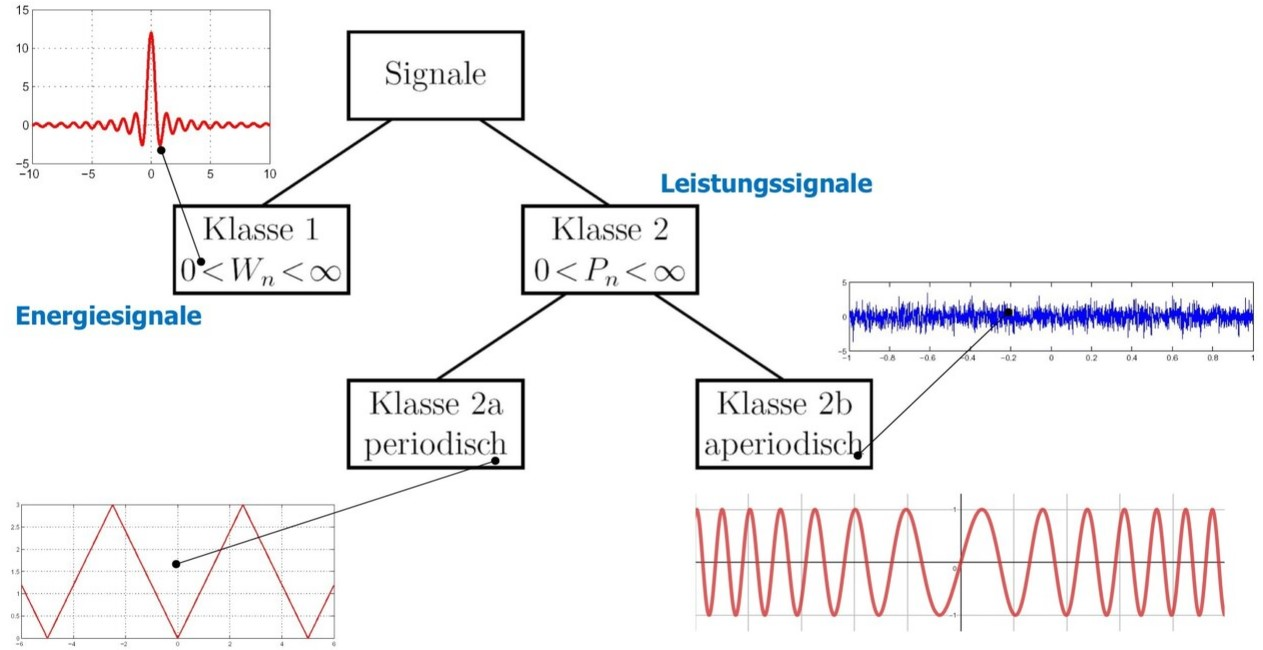
\includegraphics[width=0.85\columnwidth]{images/klassierung_signale_2.jpg}
\end{center}

Alle beschränkten Signale endlicher Dauer, die auf einem endlichen Zeitintervall von Null verschieden sind, 
sind stets Energiesignale und gehören zur Klasse 1.

\subsubsection{Normierte Signalenergie $\bm{W_n}$ / Normierte Signalleistung $\bm{P_n}$}

\begin{minipage}{0.48\columnwidth}
    $$ \boxed{ W_n = \lim\limits_{T \to \infty} \int\limits_{-T/2}^{T/2} \vert f(t) \vert ^2 \, \diff t } $$
\end{minipage}
\hfill
\begin{minipage}{0.48\columnwidth}
    $$ \boxed{ P_n = \lim\limits_{T \to \infty} \frac{1}{T} \int\limits_{-T/2}^{T/2} \vert f(t) \vert ^2 \, \diff t } $$ 
\end{minipage}

\vspace{0.2cm}

\textbf{Hinweis:} Wenn $W_n$ endlich ist, dann ist $P_n = 0$


		\section{Beschreibung von Signalen im Zeitbereich}

\textbf{Hinweis:} Sofern nichts anderes angegeben sind Signale $x(t)$ im Zeitbereich reelle Signale!


\subsection[Linearer Mittelwert]{Linearer Mittelwert $\bm{X_0 = X_m = \overline{X}}$}{5}

Der lineare Mittelwert des \textbf{reellen Signals $\bm{x(t)}$} ist definiert als:

\vspace{-0.2cm}

\begin{minipage}[t]{0.48\columnwidth}
    \begin{center}
        $$ \boxed{ X_0 = \frac{1}{T} \int\limits_{-T/2}^{T/2} x(t) \, \diff t } $$
        Klasse 2a
    \end{center}
\end{minipage}
\hfill
\begin{minipage}[t]{0.48\columnwidth}
    \begin{center}
        $$ \boxed{ X_0 = \lim\limits_{T \to \infty} \frac{1}{T} \int\limits_{-T/2}^{T/2} x(t) \, \diff t } $$
        Klasse 2b ($T$: fensterlänge, no periodo)
    \end{center}
\end{minipage}


\subsection[Quadratischer Mittelwert]{Quadratischer Mittelwert $\bm{X^2}$}{6}

Der quadratische Mittelwert von \textbf{\color{red}reellen, periodischen Leistungssignalen} (Klasse 2a) ist ein \textbf{Mass für die Leistung}
und ist definiert als:

$$ \boxed{P_n = X^2 = \frac{1}{T} \int\limits_{-T/2}^{T/2} x^2(t) \, \diff t } $$

Es gilt stets: $X^2 \geq 0$ \qquad \qquad ({\small Per Energiesignal $X^2=0$})


\subsection[Effektivwert (RMS)]{Effektivwert $\bm{X_{\rm eff}}$ (RMS)}

$$ \boxed{ X_{\rm eff} = \sqrt{X^2} = \sqrt{P_n}} $$

Es gilt: $X_{\rm eff} \geq \vert X_0 \vert$


\subsection[Mittelwert n. Ordnung]{Mittelwert $\bm{n.}$ Ordnung}{6}

Die Mittelwerte $n.$ Ordnung von \textbf{reellen, periodischen Leistungssignalen} (Klasse 2a) sind definiert als:

$$ \boxed{ X^n = \frac{1}{T} \int\limits_{-T/2}^{T/2} x^n(t) \, \diff t } $$


\subsection[Varianz]{Varianz $\bm{\Var(x) = \sigma^2}$}{7}

Die Varianz (2. zentrales Moment) ist der quadratische Mittelwert des reellen Signals $x(t)$ um $X_0$ 

$$ \boxed{ \Var(x) = \sigma^2 = \frac{1}{T} \int\limits_{-T/2}^{T/2} \big( x(t) - X_0 \big)^2  \, \diff t } $$

Es gilt stets: $\Var(x) \geq 0$


\subsection[Standardabweichung]{Standardabweichung $\bm{\sigma}$}

Wurzel der Varianz

$$ \boxed{ \sigma = \sqrt{\Var(x)} } $$


\subsection{Zusammenhänge}

Die Varianz $\Var(x)$, der quadratische Mittelwert $X^2$ und der lineare Mittelwert $X_0$ hängen folgendermassen zusammen:

$$ \boxed{ \Var(x) = \sigma^2 = X^2 - (X_0)^2 } $$

Für reelle Signale gilt:

$$ \boxed{ X^2  = \Var(x) + X_0^2 } $$


\subsection{Tipps und Tricks zur Mittelwert-Berechnung}

\begin{itemize}
	\item Skizzen machen und grafisch überlegen
	\item Integralgrenzen geschickt wählen (z.B. $0 \ldots T$ oder 2 Mal Integral mit Grenzen $0 \ldots \frac{T}{2}$)
\end{itemize}


\subsection{Übersicht wichtige Funktions-Mittelwerte}

\textbf{Hinweis:} Die Amplitude eines Signals wird als $A$ bezeichnet 

\begin{center}
    \renewcommand{\arraystretch}{1.6}
    \begin{tabular}{| l | c | c | c |}
        \hline
        \textbf{Signal}         & $\bm{X_0}$                    & $\bm{X^2} = P_n$        & $\bm{X_{\rm eff}}$                \\
        \hline
        $\sin(t)$               & $0$                           & $\frac{1}{2}$     & $\frac{\sqrt{2}}{2}$              \\
        \hline
        $\cos(t)$               & $0$                           & $\frac{1}{2}$     & $\frac{\sqrt{2}}{2}$              \\
        \hline
        $A$ (Constant)          & $A$                           & $A^2$             & $A$\\
        \hline
        $A \cdot \sin(t)$       & $0$                           & $\frac{A^2}{2}$   & $A \cdot \frac{\sqrt{2}}{2}$      \\
        \hline
        $A \cdot \cos(t)$       & $0$                           & $\frac{A^2}{2}$   & $A \cdot \frac{\sqrt{2}}{2}$      \\
        \hline
        $| A \cdot \sin(t) |$   & $| A | \cdot \frac{2}{\pi}$   & $\frac{A^2}{2}$   & $A \cdot \frac{\sqrt{2}}{2}$      \\
        \hline
        $| A \cdot \cos(t) |$   & $ | A | \cdot \frac{2}{\pi}$  & $\frac{A^2}{2}$   & $A \cdot \frac{\sqrt{2}}{2}$      \\
        \hline
        Dreieck \& Sägezahn     & $0$                           & $\frac{A^2}{3}$   &  $ A \cdot \frac{\sqrt{3}}{3}$    \\ 
        \hline
    \end{tabular}
    \renewcommand{\arraystretch}{1}
\end{center}

\textbf{Allfällige DC-Anteile der Signale ändern die Werte entsprechend!}


\subsection{Autokorrelationsfunktion (AKF)}{8-11}

L'autocorrelazione misura la somiglianza di un segnale $f(t)$ con una sua copia traslata nel tempo di un ritardo $\tau$. A differenza della convoluzione, \textbf{la funzione non viene specchiata}.

\medskip

\begin{enumerate}
    \item \textbf{Duplicare} Prendere $f(t)$ di periodo $T$ e disegnane una copia estesa su $2$ periodi per facilitare il calcolo ai bordi.
    \item \textbf{Far scorrere} Muovere la funzione mobile da SX verso DX (sfasamento $\tau$) sopra quella originale
    \item \textbf{l'area media:} Per ogni istante $\tau$, calcolare l'area di sovrapposizione $A(\tau)$ su un singolo periodo $T$ e \textbf{dividi per il periodo $T$}:
\end{enumerate}

\subsubsection{AKF für reelle, periodische Leistungssignale (Klasse 2a)}

\vspace{-0.2cm}

$$ \boxed{  \varphi_{xx}(\tau) = \frac{1}{T} \int\limits_{-T/2}^{T/2} x(t) \, x(t-\tau) \, \diff t 
    = \frac{1}{T} \int\limits_{-T/2}^{T/2} x(t+\tau) \,x(t) \, \diff t = \varphi_{xx}(-\tau) } $$

\begin{center}
    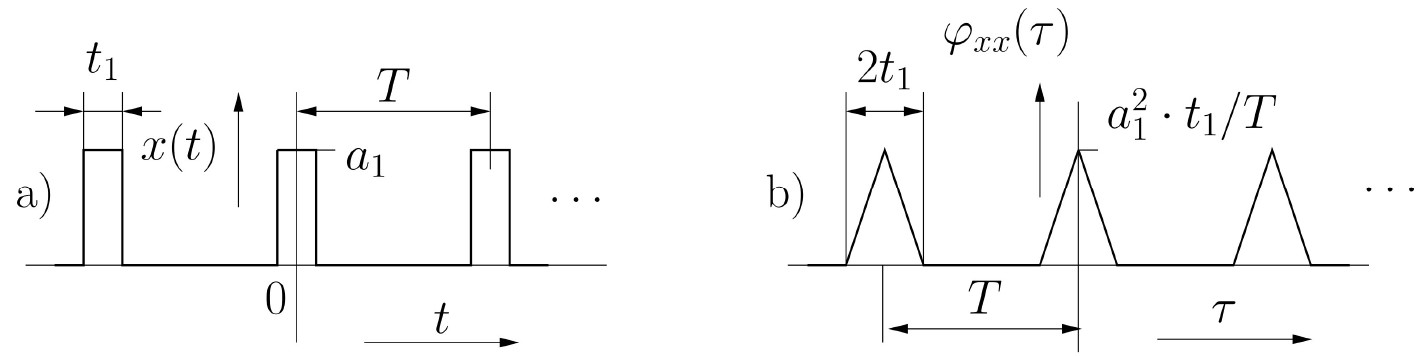
\includegraphics[width=0.8\columnwidth]{images/beispiel_AKF.jpg}
\end{center}


\subsubsection{AKF für stochastische Leistungssignale (Klasse 2b)}

\vspace{-0.2cm}

$$ \boxed{ \varphi_{xx}(\tau) = \lim\limits_{T \to \infty} \frac{1}{T} \int\limits_{-T/2}^{T/2} x(t) \, x(t-\tau) \, \diff t 
    = \lim\limits_{T \to \infty} \frac{1}{T} \int\limits_{-T/2}^{T/2} x(t+\tau) \,x(t) \, \diff t = \varphi_{xx}(-\tau) } $$


\subsubsection{AKF für Energiesignale (Klasse 1)}

\vspace{-0.2cm}

$$ \boxed{ \varphi_{xx}(\tau) = \lim\limits_{T \to \infty}  \int\limits_{-T/2}^{T/2} x(t) \, x(t-\tau) \, \diff t 
    =  \lim\limits_{T \to \infty}  \int\limits_{-T/2}^{T/2} x(t+\tau) \,x(t) \, \diff t = \varphi_{xx}(-\tau) } $$


\subsubsection{Eigenschaften der Autokorrelationsfunktion (AKF)}

\begin{itemize}
    \setlength\itemsep{5pt}
    \item $\varphi_{xx}(0) = X^2 = (X_0)^2 + \sigma^2 $ \textrightarrow\ Quadratischer Mittelwert (Definition)
    \item $\varphi_{xx}(\tau) = \varphi_{xx}(\tau \pm n \cdot T)$ mit $n \in \mathbb{N}$ \\
        d.h. die AKF ist periodisch mit der gleichen Periode $T$ wie das Signal $x(t)$ 
    \item $\varphi_{xx}(\tau) = \varphi_{xx}(-\tau)$ d.h. AKF ist \textbf{gerade Funktion} \qquad {\small Anche se $x(t)$ ungerade}
    \item $\varphi_{xx}(0) \geq \vert \varphi_{xx}(\tau) \vert$ , d.h. AKF am grössten bei vollständiger Deckung
    \item $\varphi_{xx}(\tau) \geq (X_0)^2 - \sigma^2$ 
\end{itemize}


\subsection{Kreuzkorrelationsfunktion (KKF)}{11-13}

Die KKF ist ein Mass für die \textbf{Ähnlichkeit von zwei verschiedenen} Signalen. \\
\textbf{Grafisch:} Signal $x_2$ über $x_1$ 'schieben'

\begin{itemize}
    \item nicht kommutativ
\end{itemize}

\vspace{0.2cm}

\crd{Haben $x_1$ und $x_2$ keine gemeinsamen Frequenzen, ist die KKF konstant:

$\varphi_{x_1 x_2}(\tau) = \overline{x_1}\cdot\overline{x_2}$
\textbf{(= 0, falls ein Signal mittelwertfrei ist \textrightarrow Keine DC-Offset)}}

\subsubsection{KKF für reelle, periodische Leistungssignale (Klasse 2a)}

$$ \boxed{ \varphi_{x_1 x_2}(\tau) = \frac{1}{T} \int\limits_{-T/2}^{T/2} x_1(t) \, x_2(t-\tau) \, \diff t 
    = \frac{1}{T} \int\limits_{-T/2}^{T/2} x_1(t+\tau) \, x_2(t) \, \diff t } $$

\begin{center}
    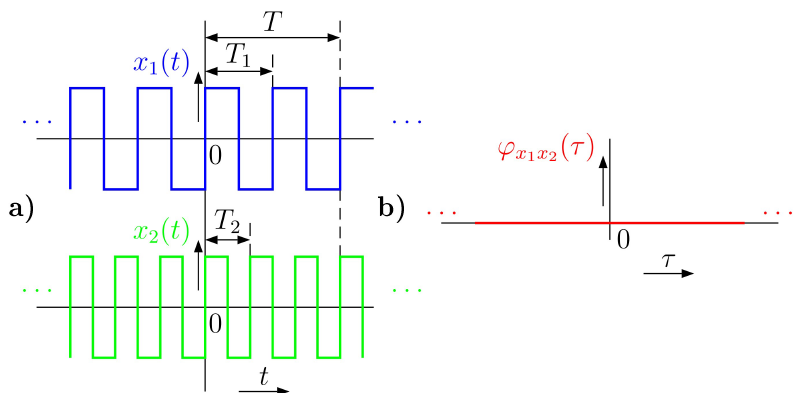
\includegraphics[width=0.7\columnwidth]{images/beispiel_KKF.png}
\end{center}


\subsubsection{KKF für stochastische Leistungssignale (Klasse 2b)}


$$ \boxed{ \varphi_{x_1 x_2}(\tau) = \lim\limits_{T \to \infty} \frac{1}{T} \int\limits_{-T/2}^{T/2} x_1(t) \, x_2(t-\tau) \, \diff t
    = \lim\limits_{T \to \infty}  \frac{1}{T} \int\limits_{-T/2}^{T/2} x_1(t+\tau) \, x_2(t) \, \diff t } $$


\subsubsection{KKF für Energiesignale (Klasse 1)}

$$ \boxed{ \varphi_{x_1 x_2}(\tau) = \lim\limits_{T \to \infty} \int\limits_{-T/2}^{T/2} x_1(t) \, x_2(t-\tau) \, \diff t 
    = \lim\limits_{T \to \infty}  \int\limits_{-T/2}^{T/2} x_1(t+\tau) \, x_2(t) \, \diff t } $$


\subsection{Faltung}{14}

\vspace{-0.2cm}

$$ \boxed{ y(t) = x_1(t) * x_2(t) = (x_1 * x_2)(t) = \int\limits_{-\infty}^{\infty} x_1(\tau) \cdot x_2(t - \tau) \; \diff \tau } $$ 


\subsubsection{Grafische Faltung}

\textbf{Grafisch:} Signal $x_2$ an $y$-Achse spiegeln und \textbf{gespiegeltes} Signal über $x_1$ 'schieben' \\
(oder umgekehrt)

\vspace{0.2cm}

\begin{tabular}{ll}
    Startpunkt: & 'Addition vom Start der beiden Supports'                              \\
    Endpunkt: 	& 'Addition vom Ende der beiden Supports'                               \\
    Maximum:	& Wenn Überlappung beider Signale am grössten                           \\
                & \textrightarrow\ nach Anzahl geschobenen Zeitschritte                 \\
    Fläche 		& Die Fläche des Faltungsprodukts entspricht der Fläche unter $x_1$ mal \\
                & der Fläche unter $x_2$         
\end{tabular}


\subsubsection{Eigenschaften des Faltungsprodukts}

\renewcommand{\arraystretch}{1.3}
\begin{tabular}{ll}
    kommutativ:     & $f * g = g * f$                   \\
    assoziativ:     & $f * (g * h) = (f * g) * h$       \\
    distributiv:    & $f * (g + h) = f * g + f * h $
\end{tabular}
\renewcommand{\arraystretch}{1}


\subsection{Komplexe Frequenzen}{15-17}

\begin{center}
    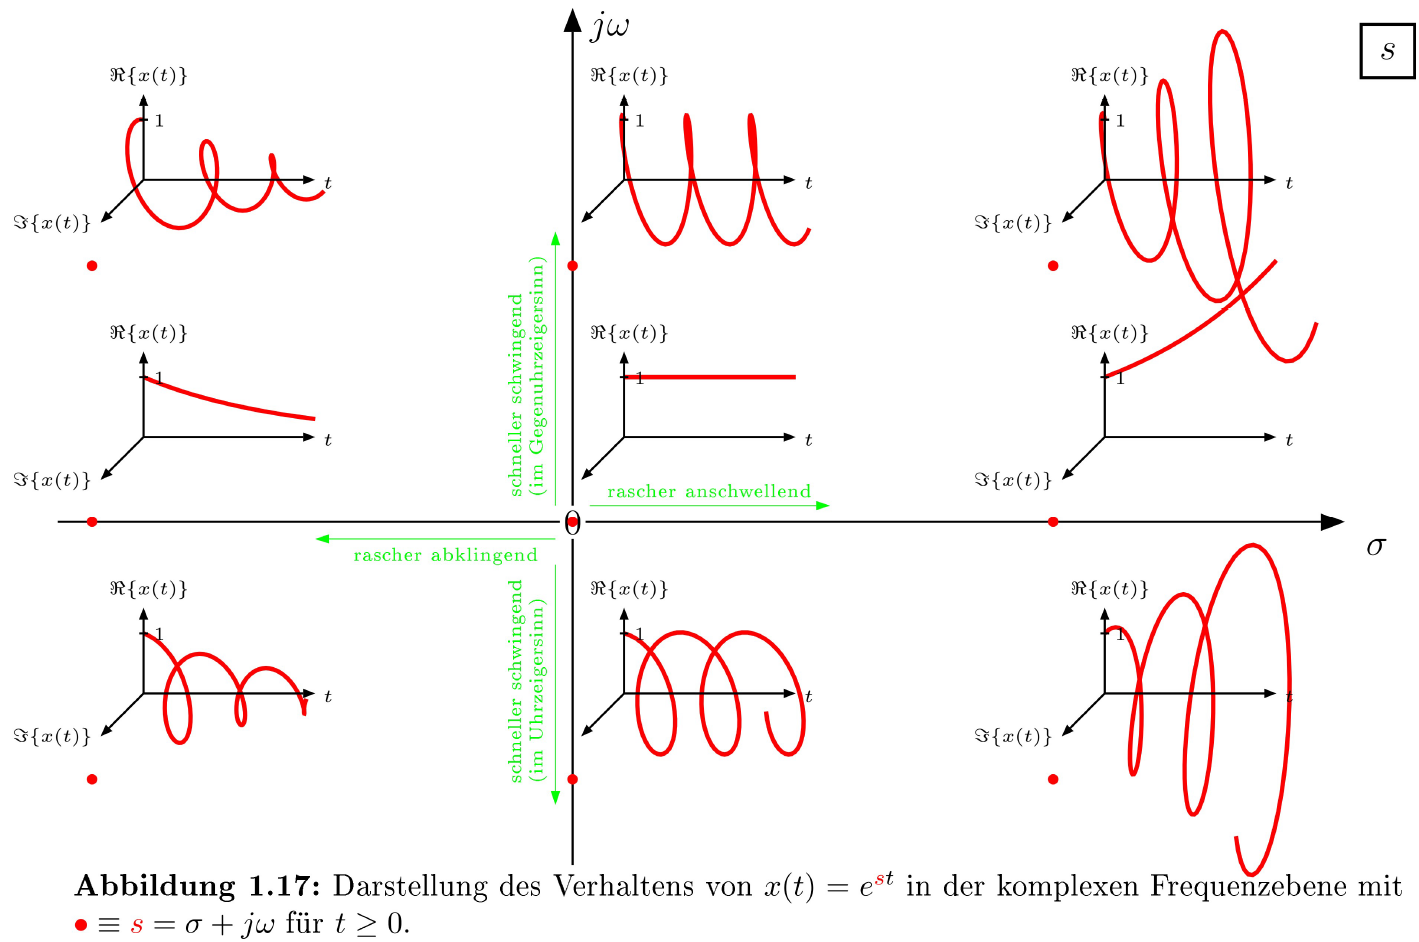
\includegraphics[width=0.88\columnwidth]{images/komplexe_frequenzen.png}
\end{center}


		\section{Wichtige Funktionen im Zeitbereich}

\subsection[Einheitssprung]{Einheitssprung $\bm{u(t)}$}{17}

\begin{minipage}[c]{0.58\columnwidth}
    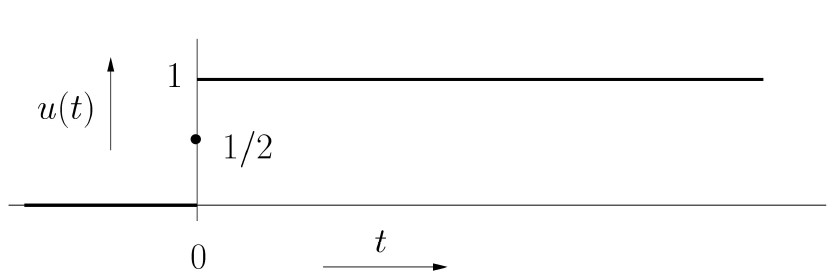
\includegraphics[width=\columnwidth]{images/einheitssprung.jpg}
\end{minipage}
\hfill
\begin{minipage}[c]{0.38\columnwidth}
    $$ u(t) = 
    \begin{cases}
        0           & \text{für } t < 0 \\
        \frac{1}{2} & \text{für } t = 0 \\
        1           & \text{für } t > 0
    \end{cases} $$

    Leistungsignal
\end{minipage}


\subsection[Signumfunktion]{Signumfunktion $\bm{\sgn(t)}$}{18}

\begin{minipage}[c]{0.48\columnwidth}
    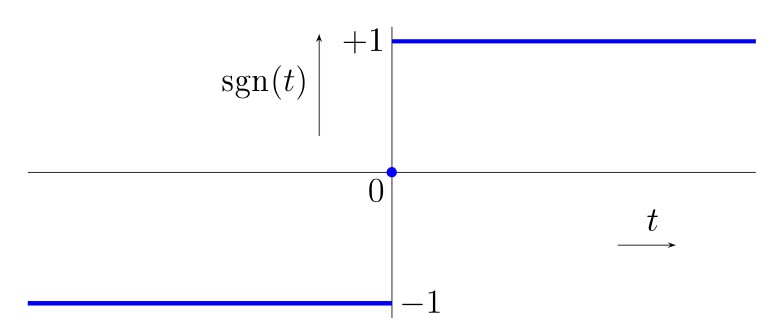
\includegraphics[width=\columnwidth]{images/signumfunktion.jpg}
\end{minipage}
\hfill
\begin{minipage}[c]{0.48\columnwidth}
    $$ \sgn(t) = 
    \begin{cases}
        -1  & \text{für } t < 0 \\
        0   & \text{für } t = 0 \\
        1   & \text{für } t > 0
    \end{cases} $$
\end{minipage}


\subsection[Rampenfunktion]{Rampenfunktion $\bm{r(t)}$}{18}

\begin{minipage}[c]{0.58\columnwidth}
    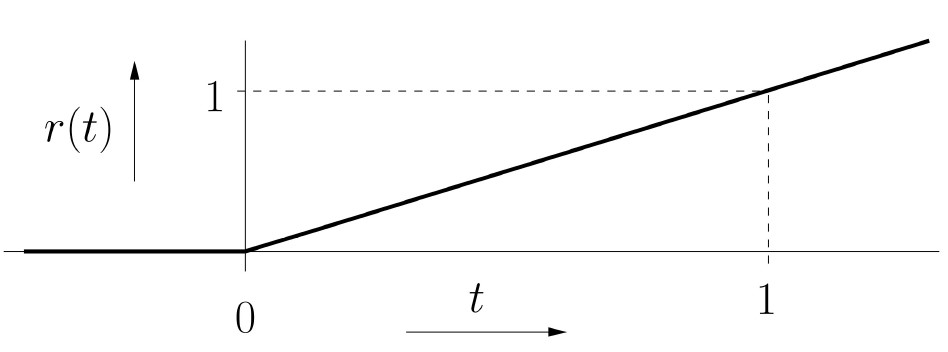
\includegraphics[width=\columnwidth]{images/rampenfunktion.jpg}
\end{minipage}
\hfill
\begin{minipage}[c]{0.38\columnwidth}
    $$ r(t) = 
    \begin{cases}
        0   & \text{für } t \leq 0 \\
        t   & \text{für } t > 0 
    \end{cases} $$
\end{minipage}


\subsection[Rechteckimpuls]{Rechteckimpuls $\bm{p_a(t)}$ \normalfont (Energiesignal)}{19}

\begin{minipage}[c]{0.58\columnwidth}
    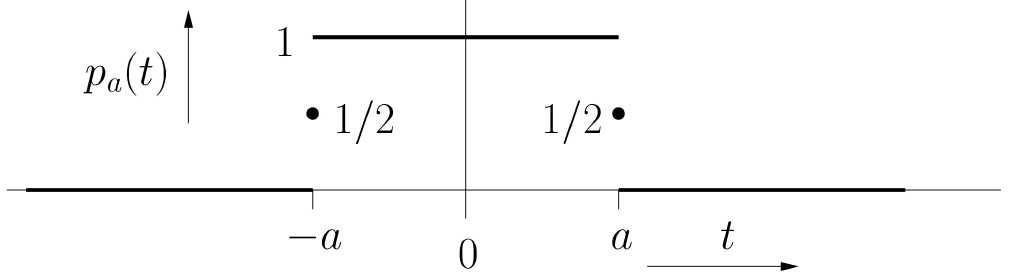
\includegraphics[width=\columnwidth]{images/rechteckimpuls.jpg}
\end{minipage}
\hfill
\begin{minipage}[c]{0.38\columnwidth}
    $$ p_a(t) = u(t+a) - u(t-a) $$
    $$ p_a(t) = 
    \begin{cases}
        1           & \text{für } \vert t \vert < a \\
        \frac{1}{2} & \text{für } \vert t \vert = a \\
        0           & \text{für } \vert t \vert > a 
    \end{cases} $$

\end{minipage}

\vspace{0.2cm}

Der Bereich von $-a$ bis $a$ heisst 'Support der Funktion'


\subsection[Dreieckimpuls]{Dreieckimpuls $\bm{\Lambda_a(t)}$}{20}

\begin{minipage}{0.5\columnwidth}
    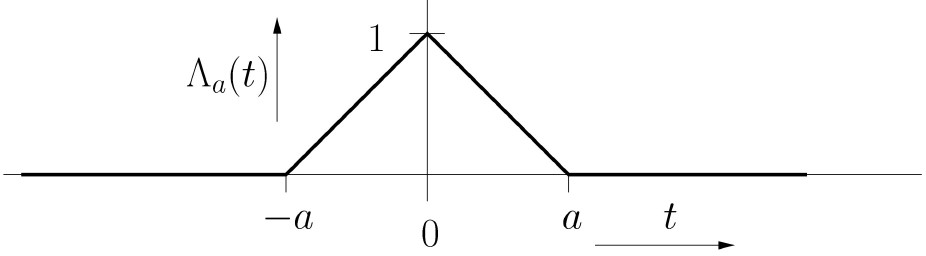
\includegraphics[width=\columnwidth]{images/dreieckimpuls.jpg}
\end{minipage}
\hfill
\begin{minipage}{0.48\columnwidth}
    $$ \Lambda_a(t) = 
    \begin{cases}
        1 - \frac{\vert t \vert}{a} & \text{für } \vert t \vert < a \\
        0                           & \text{für } |t| \geq a 
    \end{cases} $$
\end{minipage}

\vspace{0.2cm}

Der Bereich von $-a$ bis $a$ heisst 'Support der Funktion'


\subsection[Sincfunktion]{Sincfunktion $\bm{\mathrm{sinc}(t)}$}{20}

\begin{minipage}{0.48\columnwidth}
    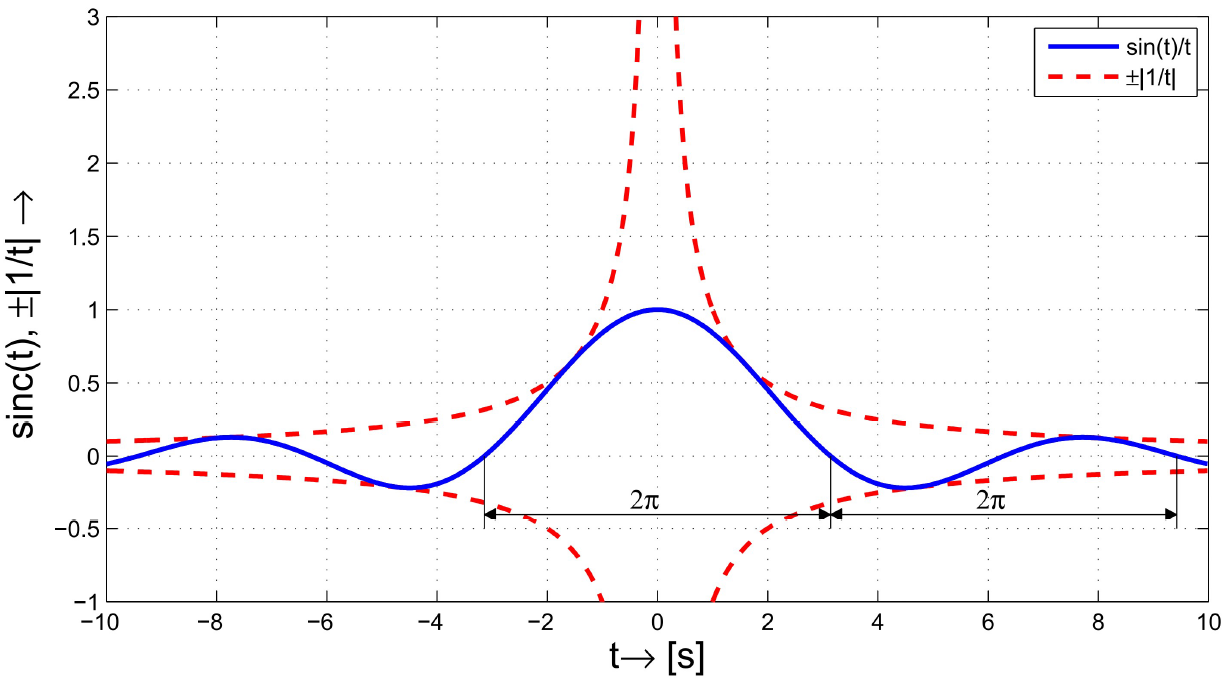
\includegraphics[width=\columnwidth]{images/sinc_funktion.png}
\end{minipage}
\hfill
\begin{minipage}{0.48\columnwidth}
    $$ \mathrm{sinc}(t) = \frac{\sin(t)}{t} \, \forall  \, t $$
\end{minipage}


\subsection[Deltafunktion (Dirac-Stoss)]{Deltafunktion (Dirac-Stoss) $\bm{\delta(t)}$}{21-23}

\begin{minipage}{0.58\columnwidth}
    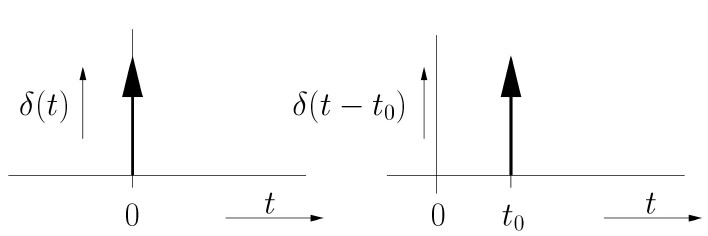
\includegraphics[width=\columnwidth]{images/deltafunktion.jpg}
\end{minipage}
\hfill
\begin{minipage}{0.38\columnwidth}
    $$ \delta(t) = 
    \begin{cases}
        \infty  & \text{für } t = 0 \\
        0       & \text{sonst}
    \end{cases} $$
        
    $$ \int\limits_{- \infty}^{\infty} \delta(t) \, \diff t = 1 $$
\end{minipage}


\subsubsection{Eigenschaften der Delta-Funktion}

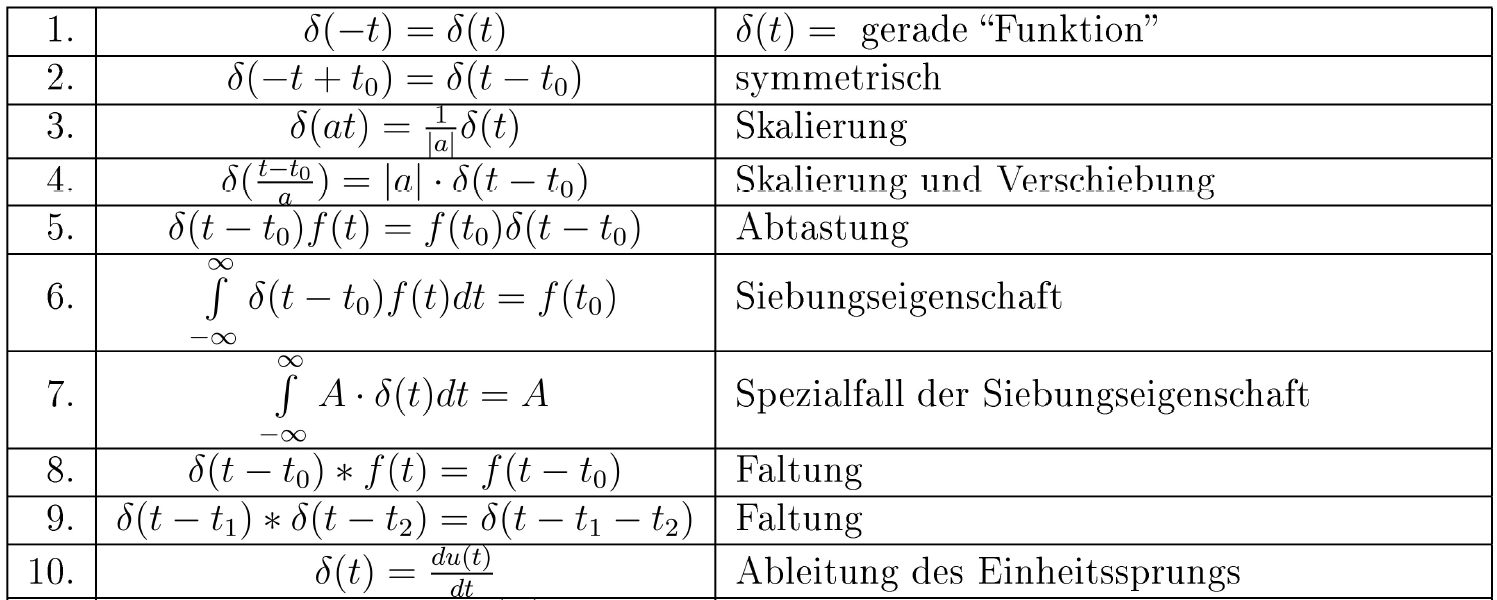
\includegraphics[width=\columnwidth]{images/eigenschaften_dirac_reduziert.png}

\vspace{0.2cm}

\textbf{\textrightarrow\ Skript S.22}


\subsection{Signalmanipulationen}{23-24}

% Von Analysis 1a Zusammenfassung

\begin{tabular}{lll}
    1.  & Streckung um $\bm{\frac{1}{a}}$ in $x$-Richtung               & $y = f(a \cdot x)$    \\
        & Spiegelung an $y$-Achse bei $\bm{-a}$ \\
    2.  & Verschiebung nach links ($\bm{+b}$) oder rechts ($\bm{-b}$)   & $y = f(x \pm b)$      \\
    3.  & Streckung um $\bm{c}$ in $y$-Richtung                         & $y = c \cdot f(x)$    \\
        & Spiegelung an $x$-Achse bei $\bm{-c}$ \\
    4.  & Verschiebung nach oben ($\bm{+d}$) oder unten ($\bm{-d}$)     & $y = f(x) \pm d $ 
\end{tabular}


\subsection{Rauschen}{25}

Rauschen bezeichnet die unregelmässige Bewegung von Ladungsträgern, welche eine Rauschspannung zur Folge hat. \\
Ist die Intensität der Rauschspannung über viele Frequenzdekaden gleich verteilt, so spricht man von weissem Rauschen.

\vspace{0.2cm}

\begin{tabular}{ll}
    \textbf{Weisses Rauschen}   & \textbf{Konstante Rauschleistung für alle Frequenzen} \\
    Farbiges Rauschen           & Frequenzabhängige Rauschleistung 
\end{tabular}

\vspace{0.2cm}

Ein \textbf{Rauschsignal} ist ein \textbf{Störsignal}, welches sich zum Nutzsignal addiert und dieses dadurch verfälscht.


\subsection{Thermisch bedingtes Rauschen (Widerstände)}

Folgende beiden Gleichungen gelten für Frequenzen bis ca. $3 \cdot 10^{12} \, \hertz$

\vspace{0.2cm}

\begin{tabular}{lll}
    $T$         & \textbf{Absolute} Temperatur                                                  & $[T] = \kelvin$                   \\
    $\Delta f$  & Bandbreite                                                                    & $[\Delta f] = \hertz$             \\
    $k$         & Boltzmann-Konstante $k = 1.380662 \cdot 10^{-23} \, \frac{\joule}{\kelvin}$   & $[k] = \frac{\joule}{\kelvin}$ 
\end{tabular}


\subsubsection{Effektive Rauschleistung $P_r$}

\vspace{-0.2cm}
$$  \boxed{ P_r = k \cdot T \cdot \Delta f } $$


\subsubsection{Effektive Rauschspannung $U_r$}

\vspace{-0.2cm}
$$  \boxed{ U_r = \sqrt{ 4 \cdot k \cdot T \cdot \Delta f \cdot R } } $$



\subsection[Signal-Rausch-Verhältnis (SNR)]{Signal-Rausch-Verhältnis (SNR) $\bm{a_r}$}{27}

Das Signal-Rausch-Verhältnis wird auch Störabstand oder Rauschabstand $a_r$ genannt. \\
Das SNR dient zur \textbf{Qualitätsbewertung von Signalen} 

$$ \boxed{ a_r = 10 \cdot \log \left( \frac{P_s}{P_r} \right) = 20 \cdot \log \left( \frac{U_s}{U_r} \right) } $$

\begin{tabular}{lll}
    $a_r$   & Störabstand / Rauschabstand / SNR     & $[a_r] = \deci \bel$  \\
    $P_s$   & Leistung des Nutzsignals              & $[P_s] = \watt$       \\
    $P_r$   & Leistung des Rauschsignals            & $[P_r] = \watt$       \\
    $U_s$   & Effektive Rauschspannung              & $[U_s] = \volt$       \\
    $U_r$   & Effektive Rauschleistung              & $[U_r] = \volt$
\end{tabular}


\subsubsection{Rauschzahl (noise figure) $F$}

Jeder Vierpol in einer Verstärkerkette (Serieschaltung) fügt dem Rauschen an seinem Eingang ein zusätzliches Rauschen hinzu. \\
Der \textbf{ausgangsseitige Rauschabstand} wird so \textbf{verkleinert}.

$$ \boxed{ F = \frac{\frac{P_{s \,\text{Eingang}}}{P_{r \,\text{Eingang}}}}{\frac{P_{s \,\text{Ausgang}}}{P_{r \,\text{Ausgang}}}}
    = \frac{P_{s \,\text{Eingang}}}{P_{r \,\text{Eingang}}} \cdot \frac{P_{r \,\text{Ausgang}}}{P_{s \,\text{Ausgang}}} } $$

Eine Rauschzahl von $F = 1$ ergibt sich einem einem \textbf{idealen Vierpol}


\subsubsection{Rauschmass $\bm{a_F}$}

Das Rauschmass $a_F$ ist die logarithmische Darstellung der Rauschzahl $F$

$$ \boxed{ a_F = 10 \cdot \log(F) = a_{r \,{\text{Eingang }}} - a_{r \,{\text{Ausgang }} } } $$ 


		\section{Amplitudenanalyse}{28}


\subsection[Amplitudendichte]{Amplitudendichte $\bm{p(a)}$}{28}

Die Amplitudendichte $p(a)$ ist ein Mass für die relative Zeit \\
(Zeit / Gesamtzeit = \textbf{Wahrscheinlichkeit}), während der sich das
Signal in einem bestimmten Amplitudenintervall aufhält 

$$ \boxed{ p(a) = \lim\limits_{\diff a \to 0} \frac{ \underbrace{ \sum t \big( a - \frac{\diff a}{2} < x(t) \leq a + \frac{\diff a}{2} \big)}_{\substack{\diff t} } }{T \cdot \diff a} 
    = \frac{1}{T} \cdot \frac{\diff t}{\diff a}  } $$

\begin{center}
    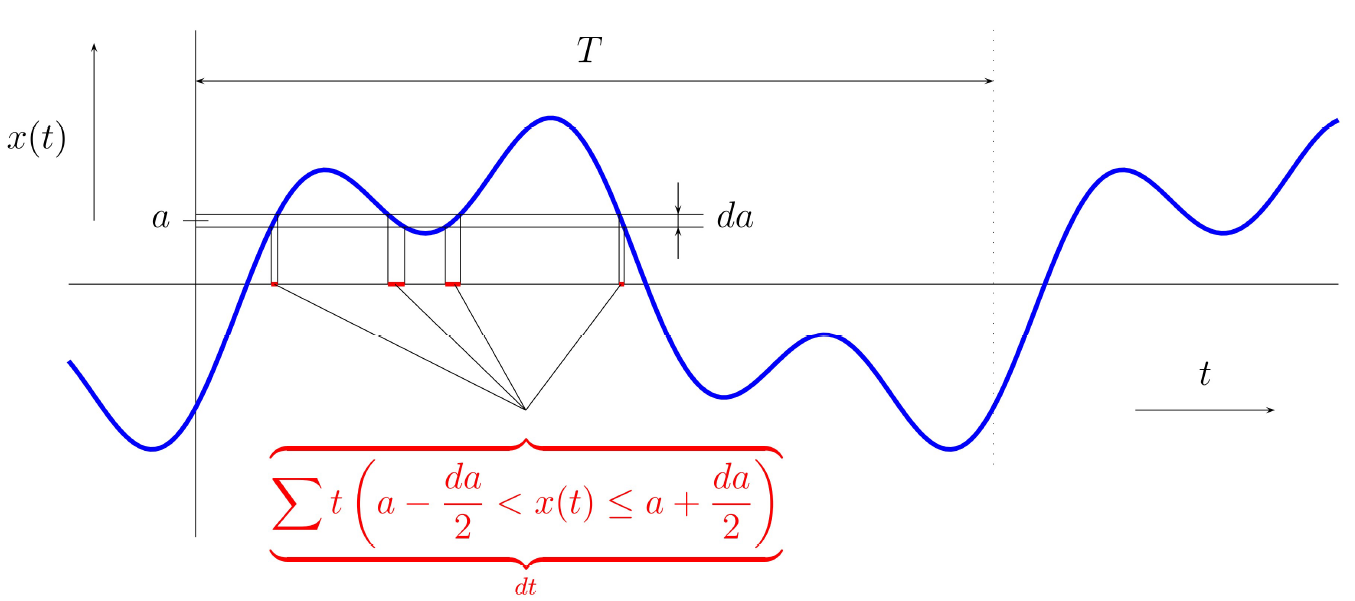
\includegraphics[width=0.75\columnwidth]{images/amplitudendichte.png}
\end{center}


\subsection[Eigenschaften der Amplitudendichte]{Eigenschaften der Amplitudendichte $\bm{p(a)}$}{28}

 \begin{itemize}
    \item  $\int\limits_{- \infty}^{\infty} p(a) \, \diff a = 1 $ \quad (Fläche = 1)
    \item Wahrscheinlichkeit, dass sich Signal in Amplitudenintervall aufhält:\\
        $ P(a_1 < a < a_2) = \int\limits_{a_1}^{a_2} p(a) \, \diff a $
    \item $p(a)$ hat \textbf{keine negativen Werte} 
 \end{itemize}

 \vspace{0.2cm}
\textrightarrow\ Weitere Informationen siehe Anhang Abschnitt ~\ref{Zusammenstellung einiger Dichtefunktionen}


\example{Amplitudendichten}

\textrightarrow\ Siehe Anhang Abschnitt ~\ref{Beispiele - Amplitudendichte}


\subsection{Addition von Amplitudendichten}{34}

Die Addition von zwei \textbf{unabhängigen} Amplitudendichten entspricht einer \textbf{Faltung}
$$ \boxed{ p_a(a) = p_1(a) * p_2(a) = \int\limits_{-\infty}^{\infty} p_1(x_1) \cdot p_2(a-x_1) \, \diff  x_1  } $$


\subsection{Mittelwerte der Amplitudendichte}{29}

\begin{minipage}[t]{0.48\columnwidth}
    \begin{center}
        \myul{\textbf{Linearer Mittelwert $\bm{X_0}$}}
        $$ \boxed{  X_0 = \int\limits_{-\infty}^{\infty} a \cdot p(a) \, \diff a } $$
    \end{center}
\end{minipage}
\hfill
\begin{minipage}[t]{0.48\columnwidth}
    \begin{center}
        \myul{\textbf{Mittelwert $\bm{n}$. Ordnung}}
        $$ \boxed{  X^n = \int\limits_{-\infty}^{\infty} a^n \cdot p(a) \, \diff a } $$
    \end{center}
\end{minipage}


\subsection{Stochastische Signale}{31}

\subsubsection{Gauss-Verteilung, Normalverteilung $\bm{N(\mu, \, \sigma)}$}

\begin{center}
    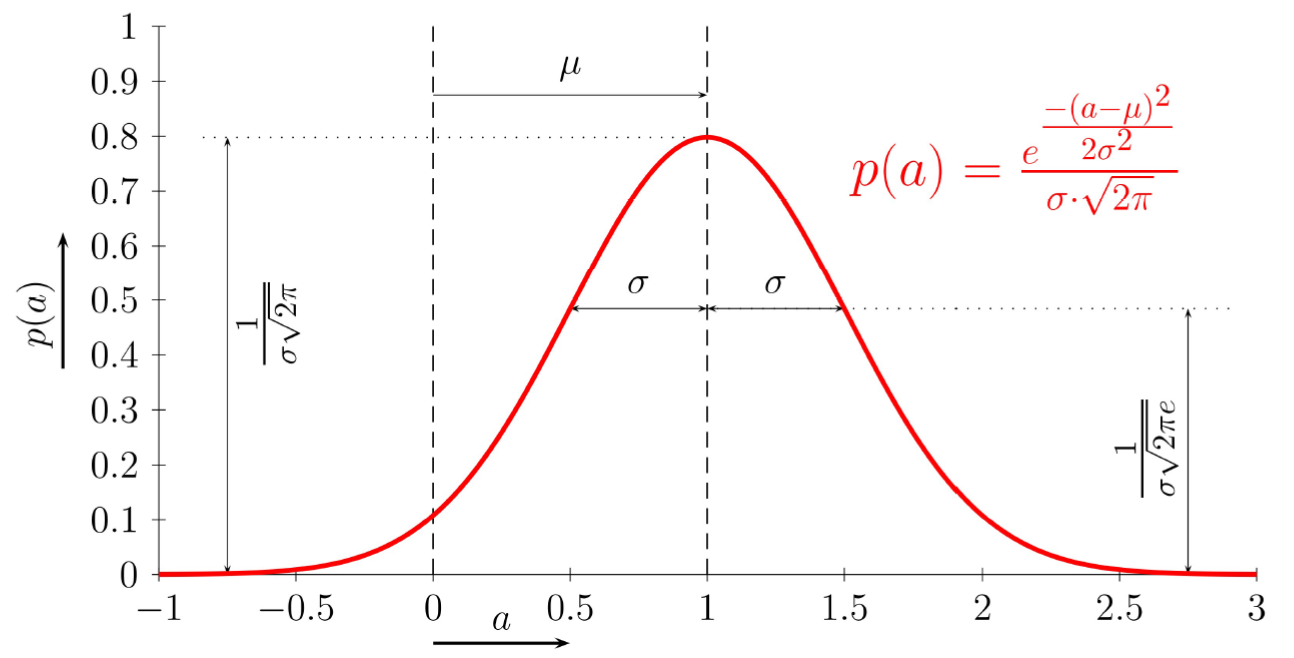
\includegraphics[width=0.8\columnwidth]{images/gaussnormalverteilung.png}
\end{center}
$$ \boxed{p(a) = N(\mu, \, \sigma) = \frac{1}{\sigma \sqrt{2 \pi}} e^{\frac{-(a -\mu)^2}{2 \sigma^2} } } $$

\vspace{0.2cm}
\textbf{Hinweis:} Werden zwei Normalverteilungen miteinander \textbf{gefaltet}, so ergibt sich wieder eine Normalverteilung:

$$ \boxed{ N(\mu_1, \, \sigma_1) * N(\mu_2, \,  \sigma_2) = 
    N \left( \underbrace{ \mu_1 + \mu_2}_{\substack{\mu}} , \, \underbrace{ \sqrt{\sigma_1^2 + \sigma_2^2} }_{\substack{\sigma}} \right) } $$


\subsubsection{Gleichverteilung}{33}

Konstante Amplitudendichte $p(a)$ in einem begrenzten Amplitudenintervall \\
\textrightarrow\ Siehe Beispiel 'Dreieck' im Anhang Abschnitt ~\ref{Dreieck} 

\columnbreak


		\section{Signalflussdiagramme (SFD)}{53}

\textbf{Grafische Darstellungen von linearen Gleichungssystemen}


\subsection{Definitionen}{53-54}

\begin{center}
    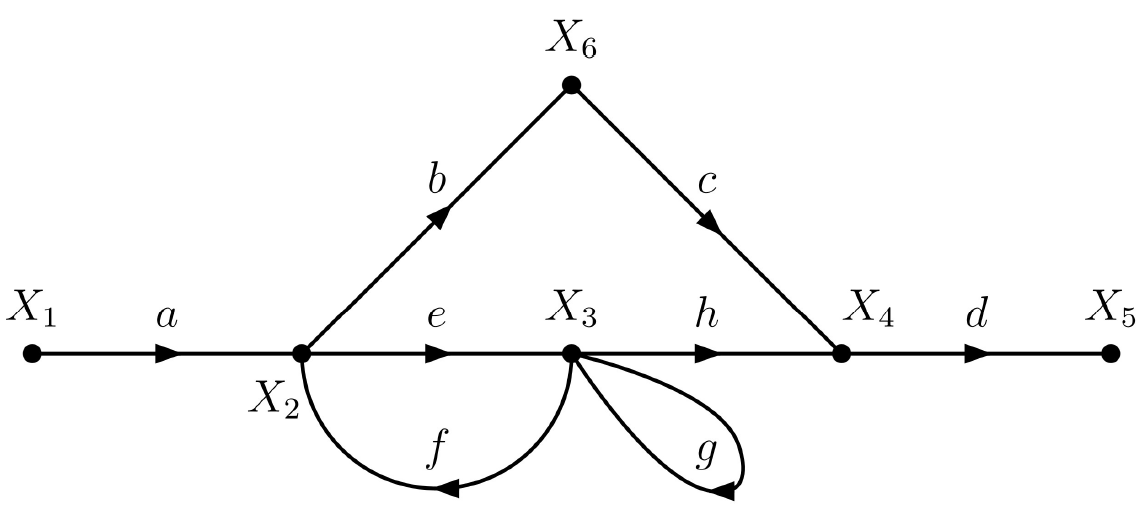
\includegraphics[width=0.75\columnwidth]{images/signalflussdiagramm.png}
\end{center}


\cbl{Der Wert einer Variablen, (Knoten) berechnet sich durch \textbf{Addition} der Zweige, die in diesen Knoten \textbf{einmünden}} 
$$\cbl{ X_4 = h \cdot X_3 + c \cdot X_6 } $$

\vspace{0.2cm}

\begin{itemize}
    \setlength\itemsep{5pt}

    \item \textbf{Knoten} Stellt bestimmte Grösse (Variable) dar ($X_1, \, X_2, \, ...$)
    \item \textbf{Zweig} Gerichtete Strecke stellt funktionale Abhängigkeit zwischen Knoten dar
    \item \textbf{Quelle} Knoten ohne einmündende Zweige ($X_1$) stellen unabh. Variable dar
    \item \textbf{Senke} Knoten ohne weggehende Zweige ($X_5$) stellen Variable dar, von welcher keine andere Variable im System abhängt
    \item \textbf{Gemischter Knoten} Knoten mit hineinführenden und weggehenden Zweigen ($X_2, \, X_3, \, X_4, \, X_6$)
    \item \textbf{Pfad} Kontinuierliche Folge von Zweigen, welche alle in die gleiche Richtung zeigen ($abcd, \, aef, \, bcd \, \ldots$)
    \item \textbf{Offener Pfad} Pfad, bei dem jeder beteiligte Knoten nur \textbf{einmal} durchquert wird
    \item \textbf{Vorwärtspfad} Offener Pfad zw. Quelle und Senke oder einem gemischten Knoten
    \item \textbf{Schleife} Geschlossener Pfad, welcher zum Ausgangsknoten zurückkehrt ($ef, \, g$)
    \item \textbf{Eigenschleife} Rückkopplungsschleife aus einem Zweig und einem Knoten ($g$)
    \item \textbf{Zweigtransmittanz} Proportionalitätskonstante zwischen zwei Knoten (Vorfaktor von Variable)
    \item \textbf{Schleifentransmittanz} Produkt der Zweigtransmittanzen einer Schleife ($ef, \, g$)
\end{itemize}


\subsection{Konstruktionsregeln}{55}

\begin{itemize}
    \item Variablen stehen bei den Knoten
    \item Signale durchqueren Zweige \textbf{nur} in Pfeilrichtung
    \item \textbf{Multiplikation} mit Transmittanzen
    \item Variable ist \textbf{Summe} der \textbf{einmündenden} Signale
    \item Variable wird auf weitergehende Zweige kopiert
\end{itemize}


\subsection{Reduktionsregeln}{59-71}

Gleichungssysteme können mit den folgenden Regeln vereinfacht werden. Die Vereinfachung entspricht einer \textbf{sukzessiven
Elimination abhängiger Variablen}.


\subsubsection{Kettentransformation}{59}

\begin{center}
    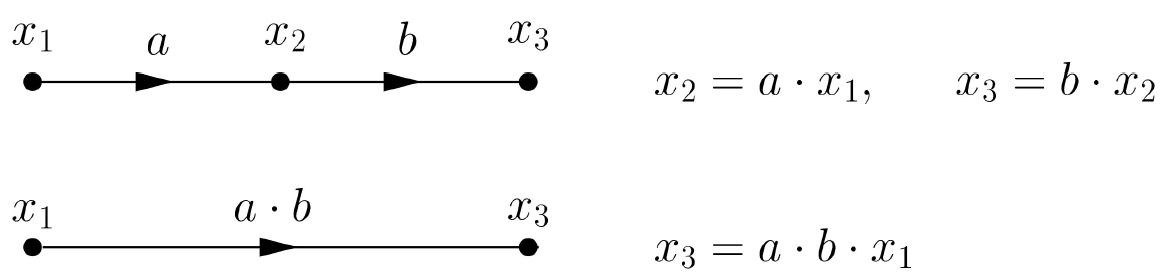
\includegraphics[width=0.8\columnwidth]{images/kettentransformation.png}
\end{center}


\subsubsection{Paralleltransformation}{59}

\begin{center}
    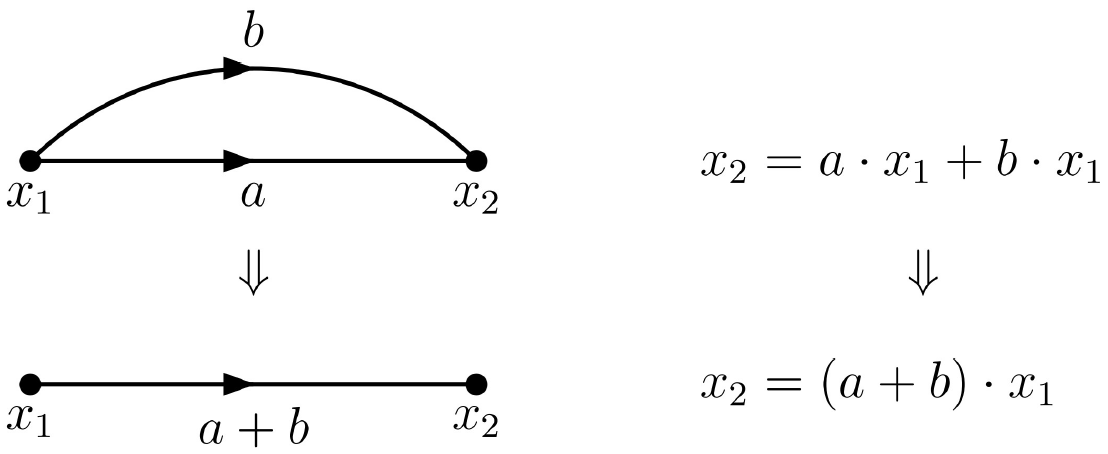
\includegraphics[width=0.7\columnwidth]{images/paralleltransformation.png}
\end{center}


\subsubsection{Entfernung eines Knotens}{60}

\begin{center}
    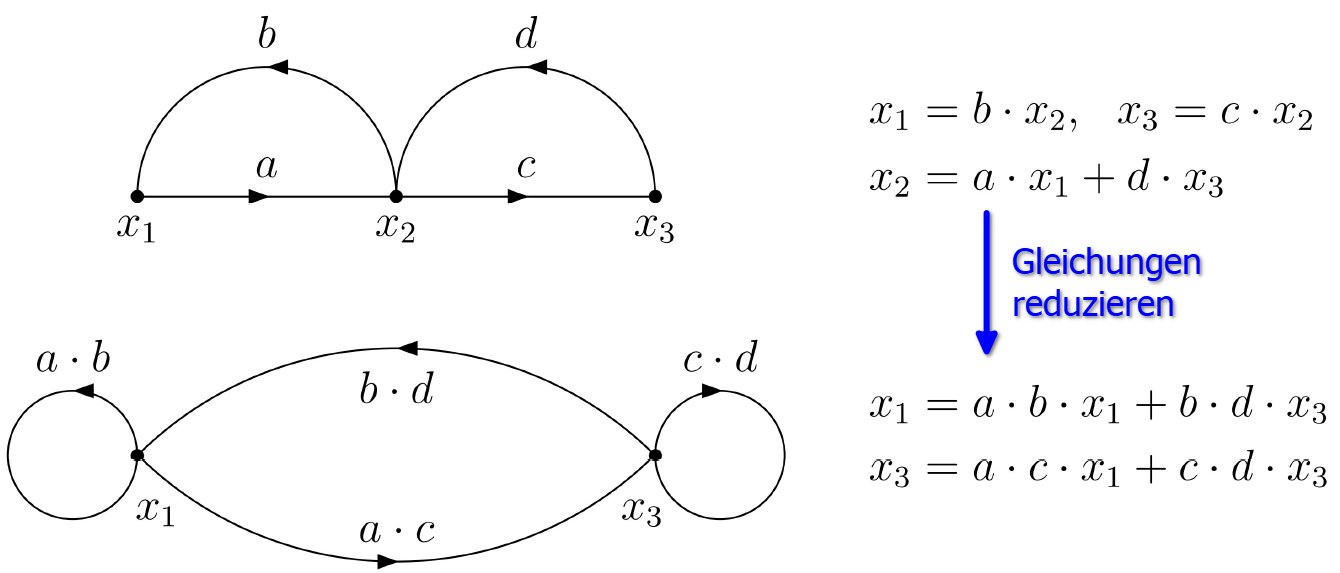
\includegraphics[width=0.85\columnwidth]{images/entfernung_knoten.png}
\end{center}


\subsubsection{Transmittanzverschiebungen}{60-61}

\textbf{Achtung:} Es muss eine neue Variable $\tilde{x_3}$ eingeführt werden, wenn der \textbf{Endpunkt eines inneren Zweiges} 
verschoben wird 

\begin{center}
    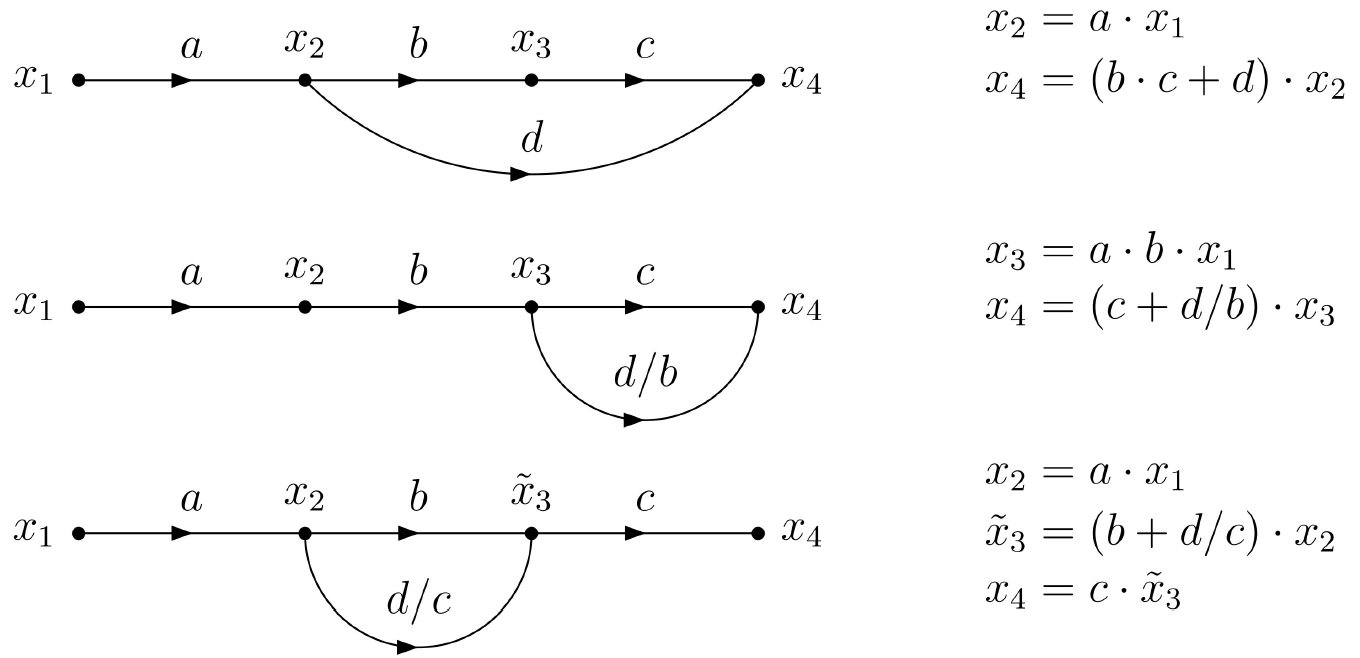
\includegraphics[width=0.85\columnwidth]{images/transmittanzverschiebung_1.png}

    \vspace{0.2cm}

    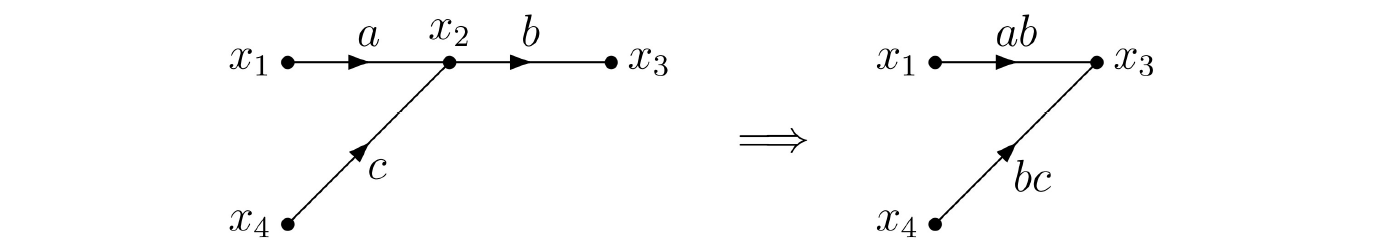
\includegraphics[width=0.75\columnwidth]{images/transmittanzverschiebung_2.png}
\end{center}



\subsubsection{Pfadinversion}{61-62}

Pfad mit Ursprung bei einer \cbl{\textbf{Quelle} $x_i$}, Endpunkt beim \cgn{Knoten $x_j$} und \textcolor{magenta}{Transmittanz $\mu$} \\
invertieren: 

\vspace{0.1cm}

\begin{itemize}
    \item Ersetzung mit Pfad von $x_j$ nach $x_i$ mit Transmittanz $1/\mu$
    \item Alle anderen Zweige, welche ursprünglich bei $x_j$ endeten so verschieben dass sie bei $x_i$ enden und ihre Transmittanzen mit $-1/\mu$ multiplizieren 
\end{itemize}

\begin{center}
    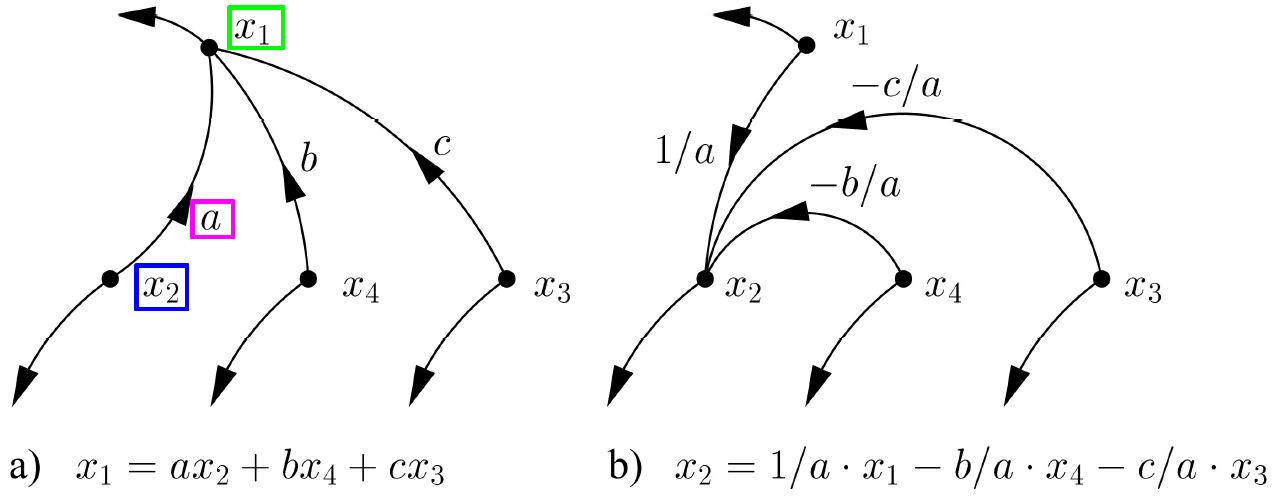
\includegraphics[width=0.9\columnwidth]{images/pfadinversion_2.png}
\end{center}

\textbf{Achtung:} Inversion eines Pfades hat Effekt, dass Quelle vom einen Ende des Pfades zum anderen Ende verschoben wird.\\
\textrightarrow\ Folge von sukzessiven Inversionen



\subsubsection{Entfernung einer Eigenschleife}{62}

Transmittanzen von allen anderen Zweigen, welche in betroffenen Knoten \textbf{einmünden} durch $(1-b)$ dividieren 

\begin{center}
    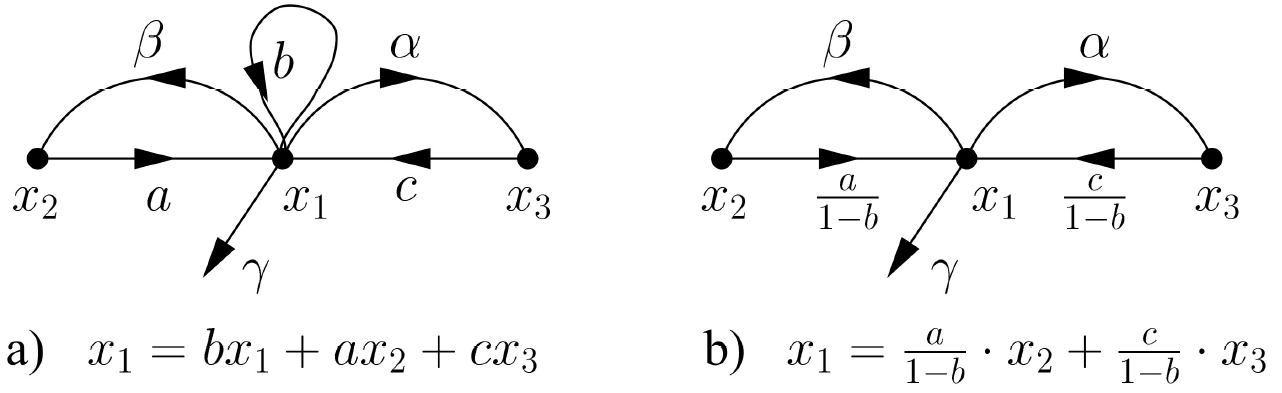
\includegraphics[width=0.8\columnwidth]{images/entfernung_eigenschleife.png} 
\end{center}


\subsubsection{Schleifenreduktion}{63-64}

\myul{\textbf{Einzelne Schleife}}

\vspace{0.1cm}

Die Transmittanz einer unabhängigen Variablen (Quelle) $x_i$ zu einer abhängigen Variablen (innerer Knoten / Senke) in einem SFD,
das nur eine Schleife und einen Vorwärtspfad enthält ist:

\vspace{0.2cm}


\begin{minipage}[c]{0.24\columnwidth}
    $$ \boxed{ H_{ij} = \frac{P_{ij}}{1-L} }$$
\end{minipage}
\hfill
\begin{minipage}[c]{0.73\columnwidth}
    \begin{tabular}{ll}
    $H_{ij}$    & Gesamte Transmittanz                                  \\ 
    $P_{ij}$    & Transmittanz des Vorwärtspfades von $x_i$ nach $x_j$  \\
    $L$         & Transmittanz der Schleife
    \end{tabular}
\end{minipage}

\begin{center}
    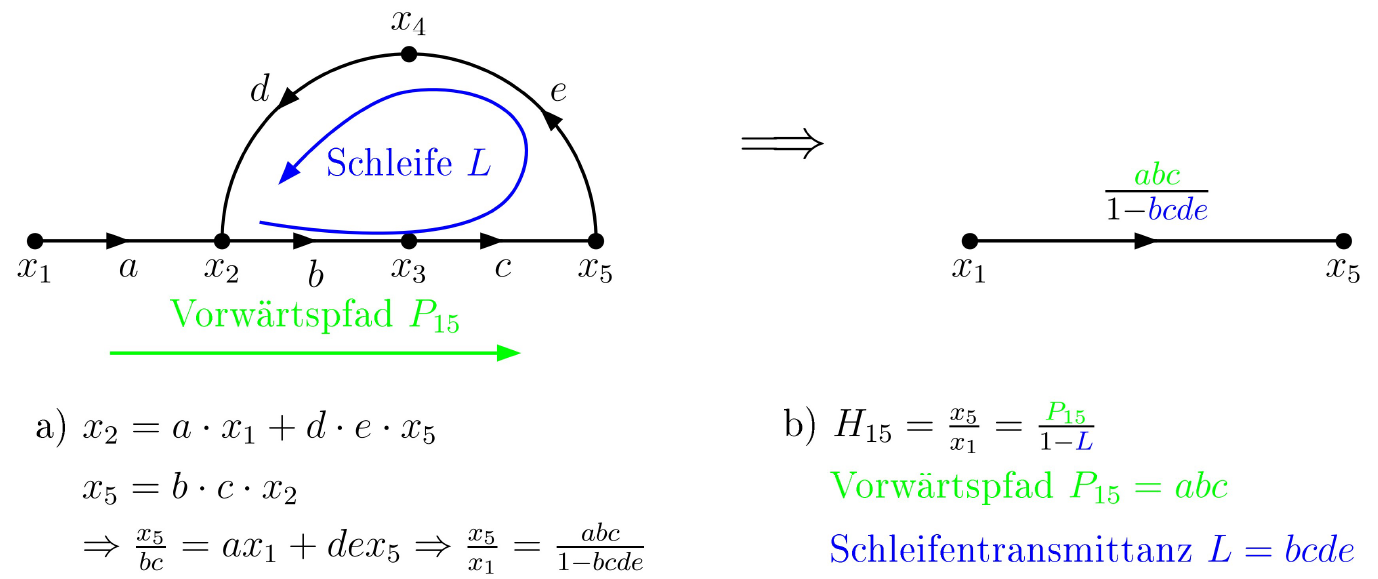
\includegraphics[width=0.9\columnwidth]{images/einzelne_schleife.png}
\end{center}

\columnbreak


\myul{\textbf{Mehrere sich nicht berührende Schleifen}}

\vspace{0.1cm}

Bei einer Kaskade von sich nicht berührenden Schleifen (d.h., dass sie \textbf{keinen gemeinsamen Knoten} haben) ist die gesamte
Transmittanz gegeben durch: 

\vspace{0.2cm}

\begin{minipage}[c]{0.45\columnwidth}
    $$ \boxed{ H_{\rm in} = \frac{P_{ij}}{1-L_j} \cdot\frac{P_{jk}}{1-L_k} \cdot \ldots \cdot \frac{P_{(n-1)n}}{1-L_n} } $$
\end{minipage}
\hfill
\begin{minipage}[c]{0.5\columnwidth}
    \begin{tabular}{ll}
        $H_{\rm in}$& Gesamte Transmittanz              \\ 
        $P_{ij}$    & Transmittanz des Vorwärtspfades   \\
                    & von $x_i$ nach $x_j$              \\
        $L$         & Transmittanz der Schleife 
    \end{tabular}
\end{minipage}

\begin{center}
    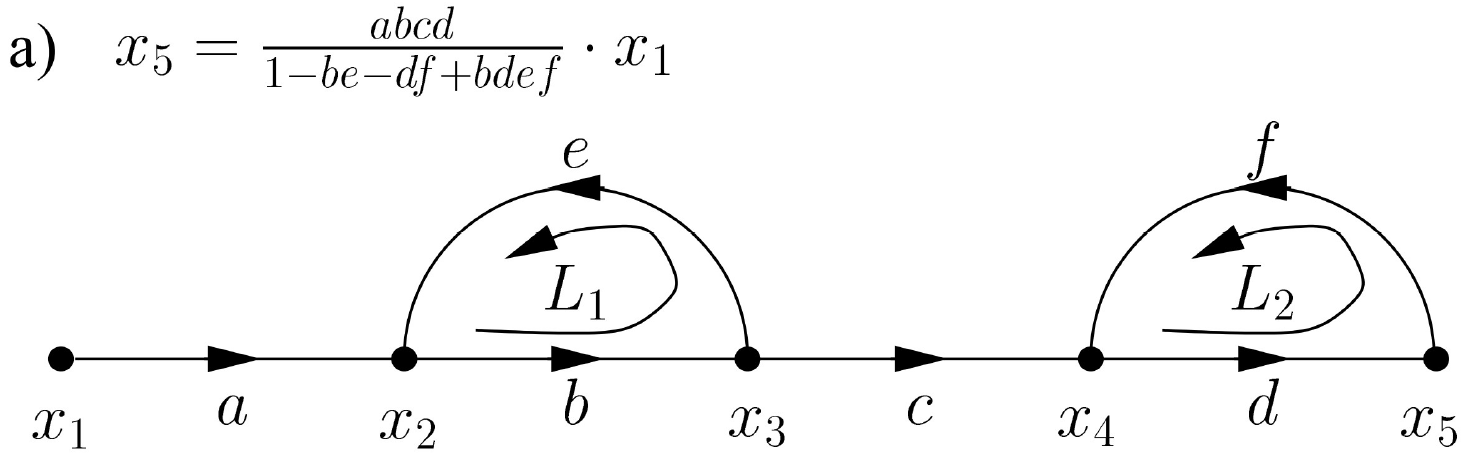
\includegraphics[width=0.8\columnwidth]{images/nicht_beruehrende_schleifen.png}
\end{center}


\myul{\textbf{Mehrere sich berührende Schleifen}}

Für den Fall, dass zwei Schleifen mind. einen \textbf{gemeinsamen Knoten} haben, ist die gesamte Transmittanz gegeben durch:

\begin{center}
    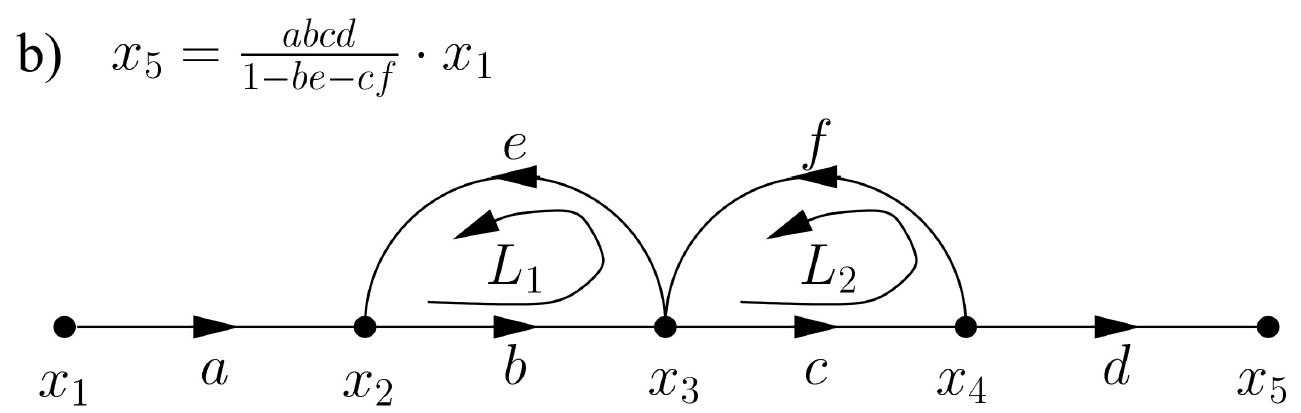
\includegraphics[width=0.8\columnwidth]{images/beruehrende_schleifen.png} 
\end{center}


\subsubsection{Allg. Mehrfachschleifen-Reduktionsregel für einfache Pfade}

Es existiert \textbf{nur ein Pfad} zwischen einer Quelle $x_i$ und einem abhängigen Knoten $x_j$, wobei dieser Pfad jede Schleife
im SFD berührt (d.h., dass er \textbf{wenigstens einen Knoten mit jeder Schleife} gemeinsam hat)

\vspace{0.2cm}

\begin{minipage}{0.25\columnwidth}
    $$ \boxed{ H_{ij} = \frac{x_j}{x_i} = \frac{P_{ij}}{\Delta} } $$
\end{minipage}
\hfill
\begin{minipage}{0.7\columnwidth}
    \begin{tabular}{ll}
        $H_{ij}$    & Gesamte Transmittanz              \\ 
        $P_{ij}$    & Transmittanz des Vorwärtspfades   \\
                    & von $x_i$ nach $x_j$              \\
        $\Delta$    & Graph- / Netzwerkdeterminante
    \end{tabular}
\end{minipage}

\vspace{0.2cm}

\fcolorbox{red}{white}{\parbox{0.97\columnwidth}{
 $\Delta = $ 1 \cor{$-$} (Summe aller Schleifen) \cor{$+$} (Summe aller Produkte zweier Schleifen, die sich \textbf{nicht berühren}) 
    \cor{$-$} (Summe aller Produkte dreier Schleifen, die sich \textbf{nicht berühren}) \cor{$+$} $\ldots$}}
 
\begin{center}
    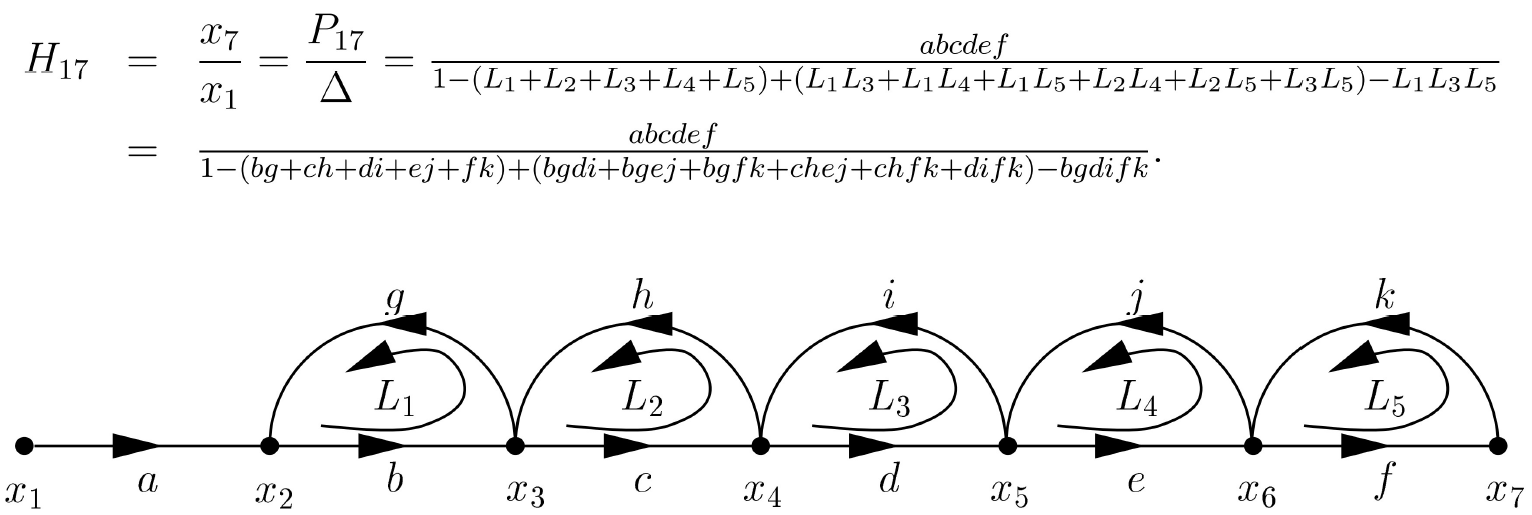
\includegraphics[width=0.9\columnwidth]{images/beispiel_schleifenreduktion.png}
\end{center}

\textrightarrow\ \textbf{Schleifen dürfen auch innerhalb von Schleifen sein}


\subsubsection{Mason's Regel}{27-71}

 
\begin{minipage}{0.4\columnwidth}
    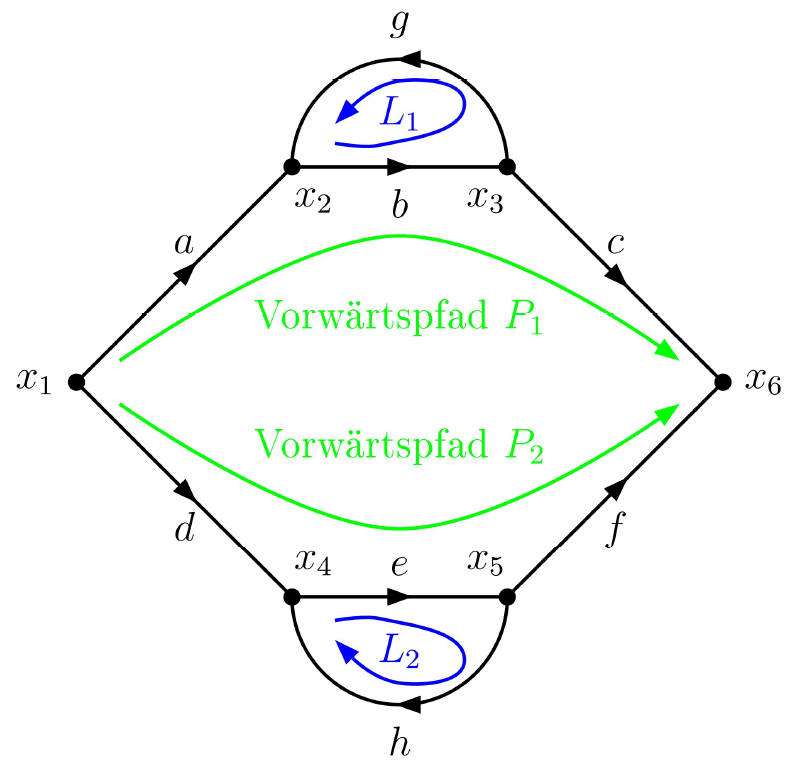
\includegraphics[width=\columnwidth]{images/mason_regel.png}
\end{minipage}
\hfill
\begin{minipage}{0.48\columnwidth}
    \raggedright

    $$ \boxed{ H_{ij} = \frac{x_j}{x_i} = \frac{\sum\limits_k (P_k \cdot \Delta_k )}{\Delta} } $$

    \vspace{0.2cm}

    \crd{\textbf{$x_i$ muss eine Quelle sein!}} \\
    $x_j$ kann eine Senke oder ein gemischter Knoten sein 
\end{minipage}

\vspace{0.2cm}

    \begin{tabular}{ll}
    $H_{ij}$    & Gesamte Transmittanz                                                          \\ 
    $P_{k}$     & Transmittanz des k-ten offenen Pfades zwischen $x_i$ und $x_j$                \\
    $\Delta$    & Graph- / Netzwerkdeterminante                                                 \\
    $\Delta_k$  & Kofaktor (Kodeterminante) \textrightarrow\ siehe \crd{rote} Box               \\
                & Schleifentransmittanzen, welche k-ten Vorwärtspfad \textbf{nicht} berühren    \\
                & \textrightarrow\ siehe \crd{rote} Box
\end{tabular}

\vspace{0.2cm}

\textbf{Es gibt gleich viele Kofaktoren wie Vorwärtspfade}

\vspace{0.2cm}

\textbf{Wenn $\bm{x_i}$ (hier als Beispiel $\bm{x_2}$) keine Quelle ist:} 
$$ \cbl{ H_{23} = \frac{x_3}{x_2} = \frac{\frac{x_3}{x_1}}{\frac{x_2}{x_1}} 
    = \frac{H_{13}}{H_{12}} = \frac{\frac{P_4 \Delta_4 + P_5 \Delta_5}{\Delta}}{\frac{P_1 \Delta_1 + P_2 \Delta_2 + P_3 \Delta_3}{\Delta}} 
    \quad \text{ \textrightarrow\ } \Delta \text{ streicht sich} }$$



\example{Beispiel Mason's Regel}

\begin{center}
    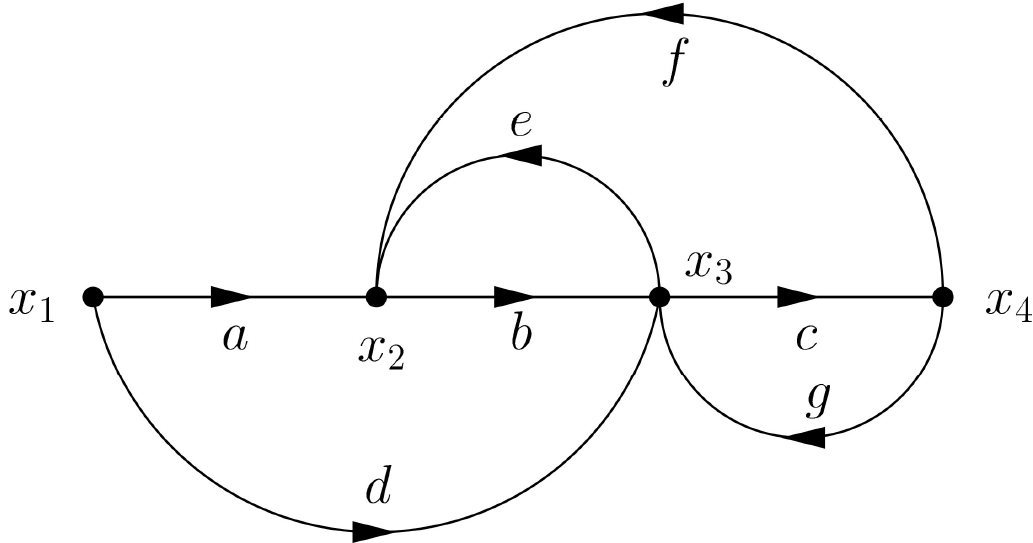
\includegraphics[width=0.65\columnwidth]{images/mason_beispiel_1.png} 
\end{center}


\myul{\textbf{$\bm{x_1}$ ist Quelle:}}

\begin{center}
    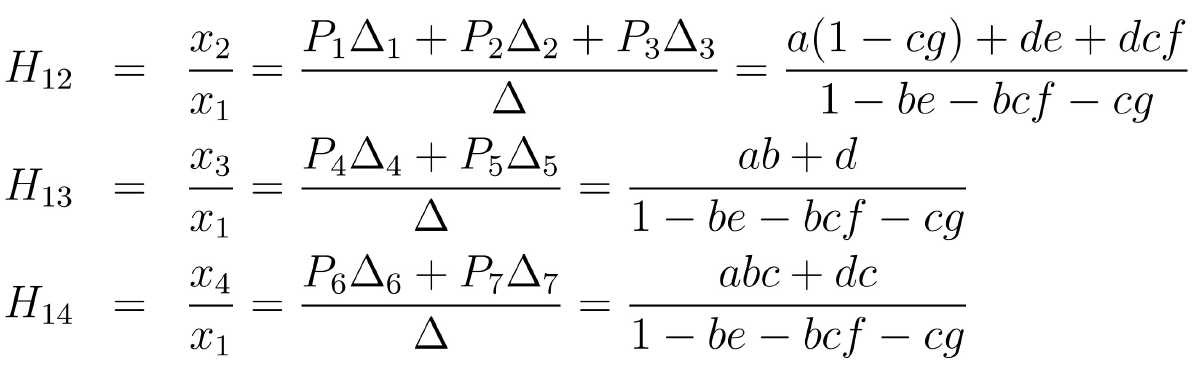
\includegraphics[width=0.8\columnwidth]{images/mason_beispiel_2.png}
\end{center}


\cbl{\myul{\textbf{$\bm{x_2}$ ist keine Quelle:} }}

\vspace{0.2cm}

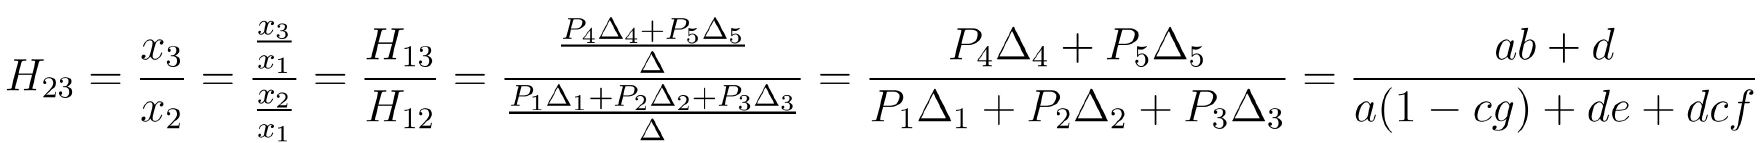
\includegraphics[width=\columnwidth]{images/mason_beispiel_3.png} 


\subsection{Ordnung eines SFD}{72}

Die Ordnung eines SFDs entspricht der \textbf{minimalen Anzahl Knoten}, welche \textbf{entfernt} werden müssen, 
um \textbf{alle Schleifen aufzubrechen}. \\
Diese zu entfernenden Knoten heissen \cbl{\textbf{fundamentale Knoten}} 

\vspace{0.2cm}

\textbf{Hinweis:} 'Entfernen' bedeutet, den Knoten ersatzlos zu streichen (und somit Pfade bzw. die \textbf{Schleifen} zu zerstören)

\begin{center}
    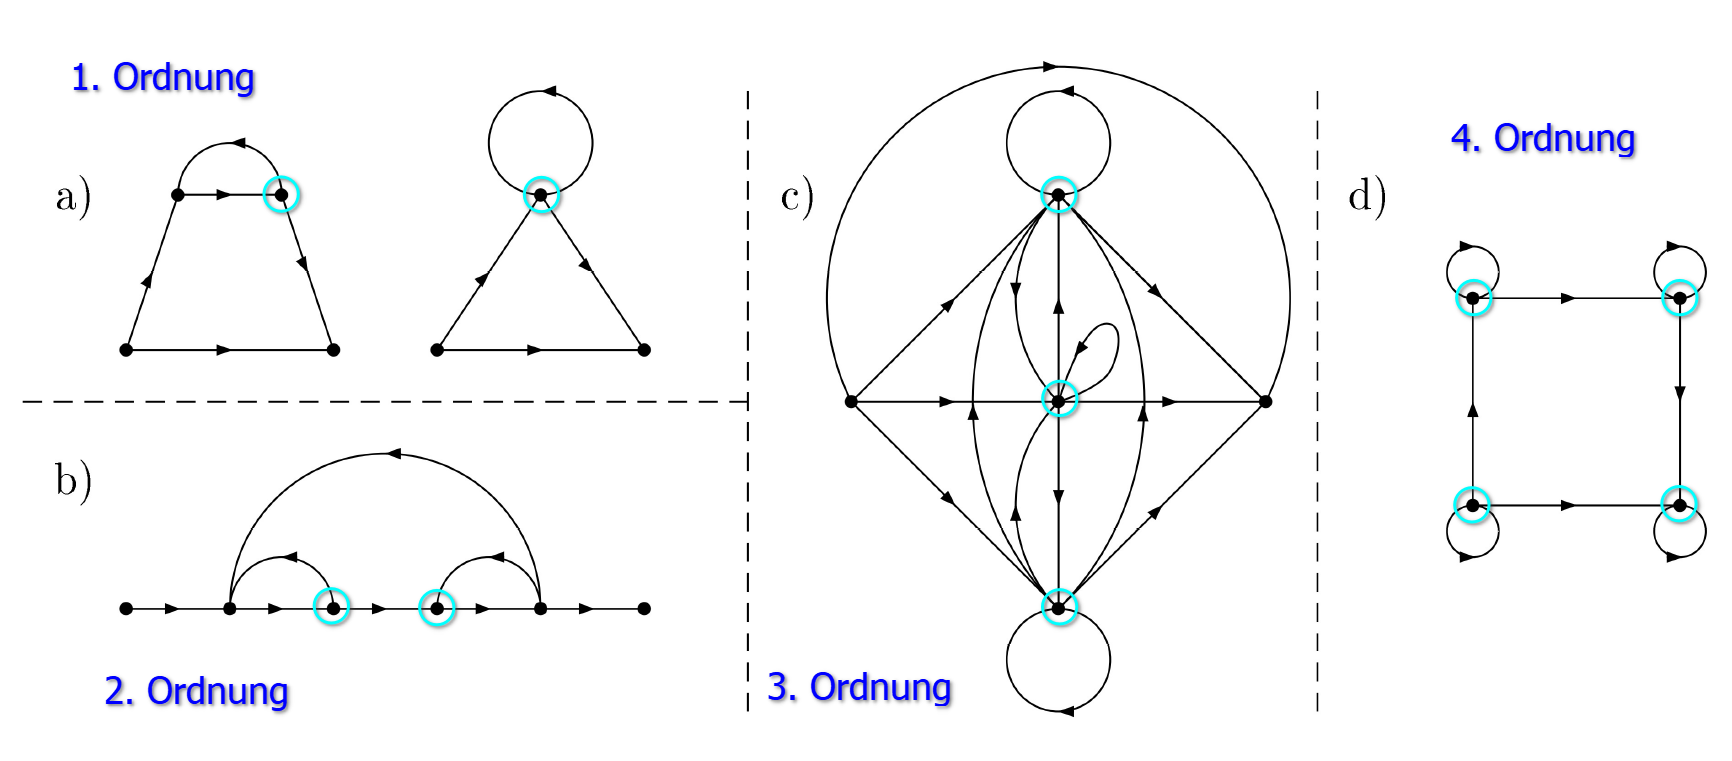
\includegraphics[width=0.9\columnwidth]{images/ordnung_SFD.png}
\end{center}

\textrightarrow\ Die \textbf{Ordnung eines SFDs} entspricht im Allgemeinen \textbf{nicht der Ordnung} des dazugehörigen \textbf{Systems}


\subsection{Fundamentales SFD 1. Ordnung}{73}

\begin{minipage}{0.27\columnwidth}
    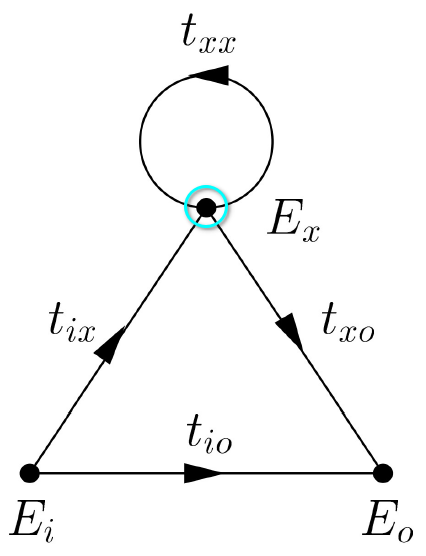
\includegraphics[width=\columnwidth]{images/fundamentales_SFD_ordnung_1.png} 
\end{minipage}
\hfill
\begin{minipage}{0.66\columnwidth}
    \begin{tabular}{ll}
        $E_x$       & Fundamentaler Knoten                      \\
        $E_i$       & Eingangsknoten (Quelle)                   \\
        $E_o$       & Ausgangsknoten (Senke)                    \\
        $t_{io}$    & Totale Transmittanz von $E_i$ zu $E_o$    \\
        $t_{ix}$    & Totale Transmittanz von $E_i$ zu $E_x$    \\
        $t_{xo}$    & Totale Transmittanz von $E_x$ zu $E_o$    \\
        $t_{xx}$    & Totale Transmittanz von $E_x$ zu $E_x$ 
    \end{tabular}
\end{minipage}


\subsubsection{Übertragungsfunktion UTF eines SFD 1. Ordnung}

\vspace{-0.2cm}
$$ \boxed{ H_{io} = \frac{E_o}{E_i} = t_{io} + \frac{t_{ix} \, t_{xo}}{1 - t_{xx}} = 
    \frac{t_{io} - t_{io} \, t_{xx} + t_{ix} \, t_{xo}}{1- t_{xx}}} $$

\textbf{Die Parameter $\bm{t_{io}}$, $\bm{t_{ix}}$, $\bm{t_{xo}}$ und $\bm{t_{xx}}$ müssen gemäss obiger Tabelle bestimmt werden}


\subsection{Transposition}{85-86}

Die Transposition ist eine wichtige Methode für die Ableitung von \textbf{alternativen praktischen Topologien} mit \textbf{identischen UTF}


\subsubsection{Vorgehen Transposition}

\begin{enumerate}
   \item Richtungsumdrehung aller Zweigtransmittanzen bei gleichbleibenden Transmittanzen 'Pfeile umdrehen' 
   \item Spiegelung des resultierenden SFD
   \item Bezeichnungswechsel von Eingangs- und Ausgangsknoten
\end{enumerate}

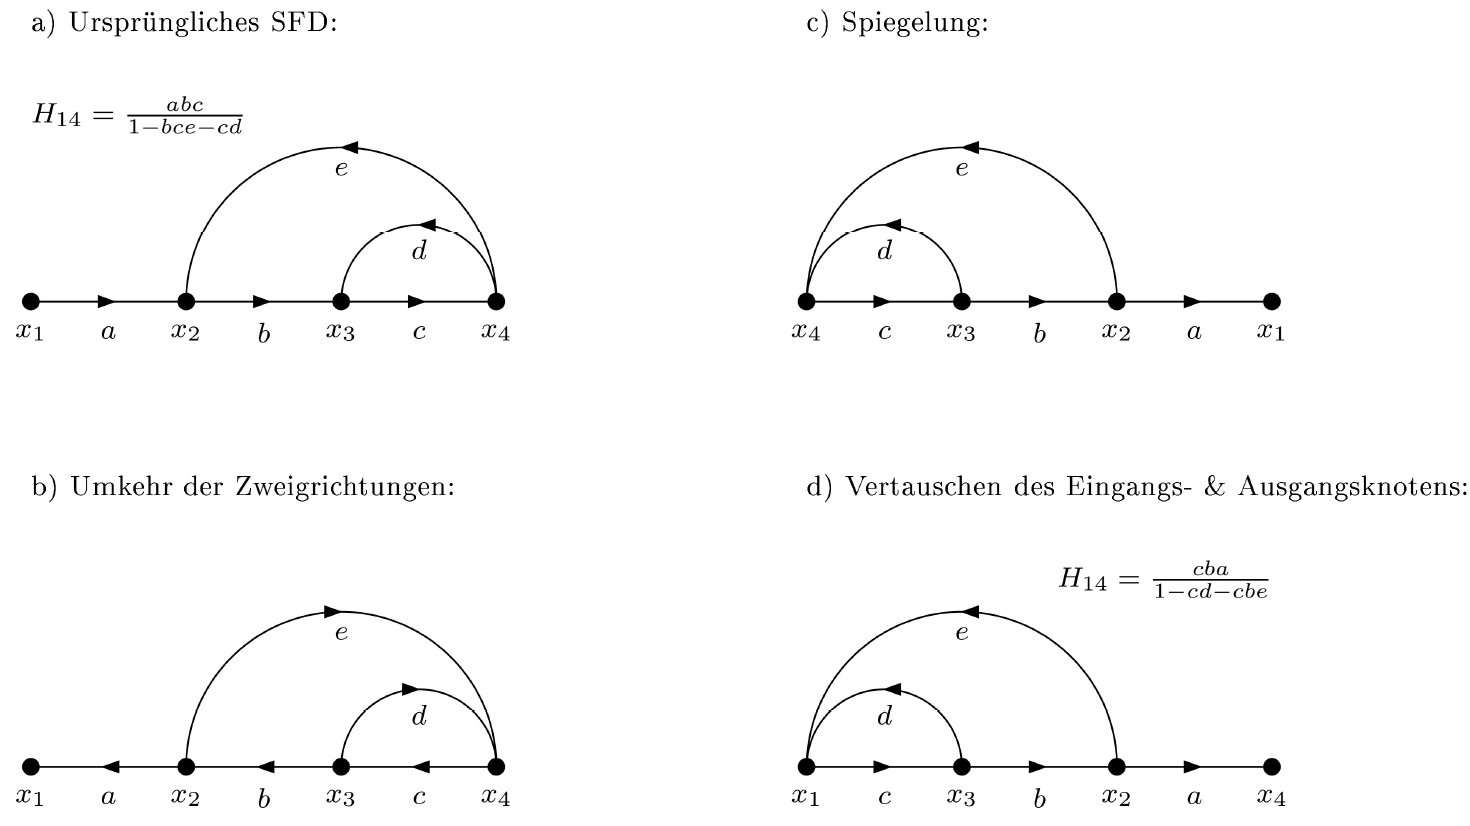
\includegraphics[width=\columnwidth]{images/transposition.png} 


\subsubsection{Inversion vs. Transposition}

Bei der \textbf{Inversion} enthält das resultierende SFD nur noch Vorwärtspfade und keine Rückkopplungsschleifen. \\
Die Resultierende nichtkausale Funktion ist die Summe aller Pfade von der neuen Quelle zur neuen Senke.

\vspace{0.2cm}

\scalebox{0.9}{
\begin{tabular}{l c c c l}
    $H_{14}$                                                & \textrightarrow\  & Invertierung  & \textrightarrow\  & $\tilde{H}_{41} = \frac{1}{H_{14}}$ \\
    \\
    $ H_{14} = \frac{x_4}{x_1} = \frac{abc}{1-bce - cd} $   &                   &               &                   & $\tilde{H}_{41} = \frac{1}{abc} - \frac{e}{a} - \frac{d}{ba} = \frac{1 - bce - cd}{abc} =  \frac{1}{H_{14}}$ 
    \end{tabular}
}

\vspace{0.2cm}

\begin{center}
    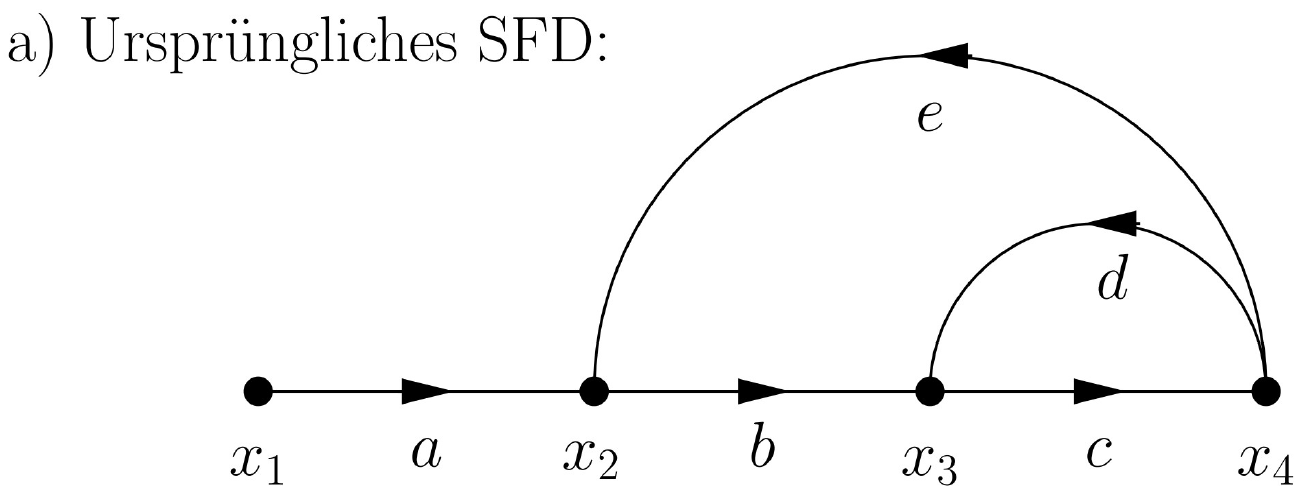
\includegraphics[width=0.45\columnwidth]{images/transposition_vs_invertierung_1.png}
\end{center}

\begin{minipage}[c]{0.48\columnwidth}
    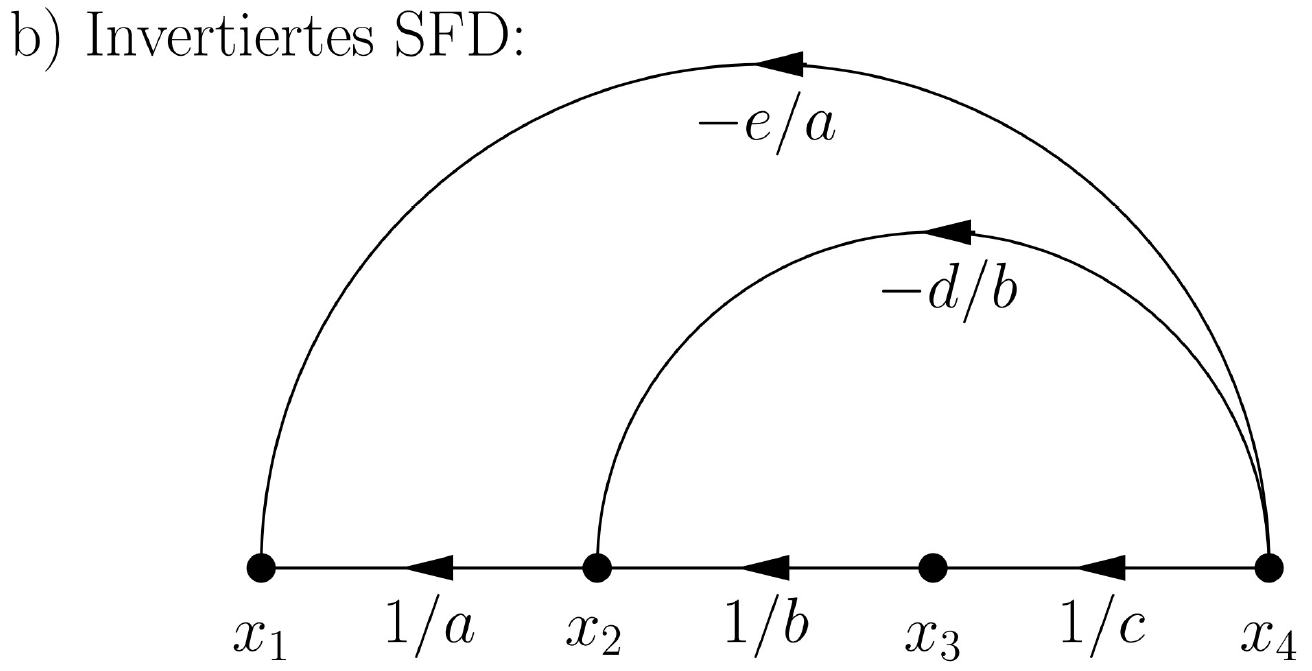
\includegraphics[width=0.9\columnwidth]{images/transposition_vs_invertierung_2.png}
\end{minipage}
\hfill
\begin{minipage}[c]{0.48\columnwidth}
    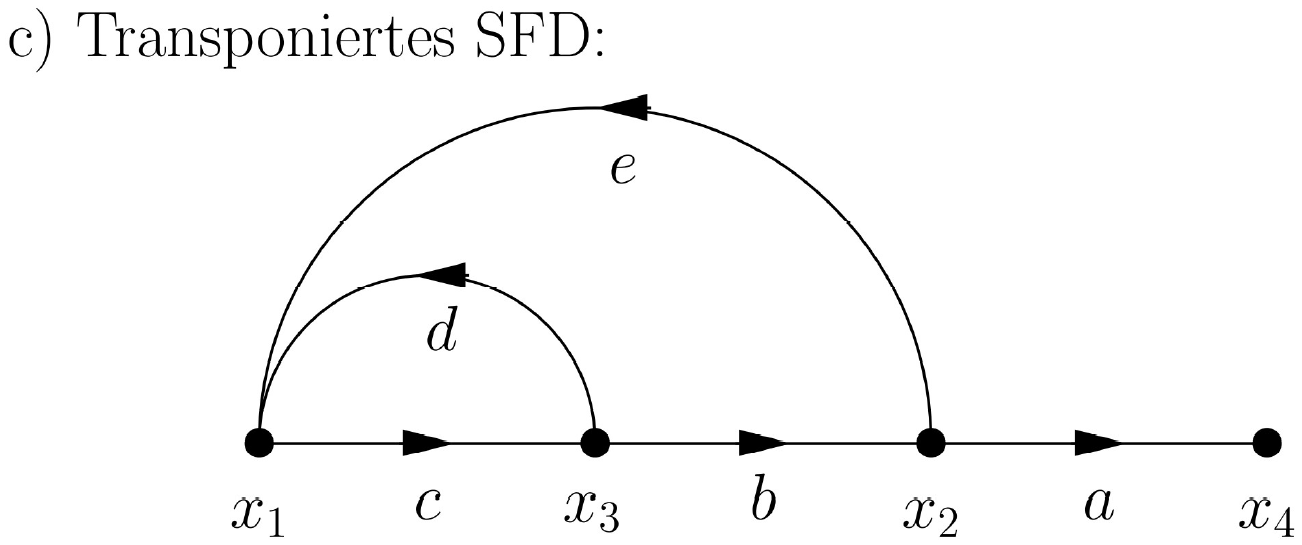
\includegraphics[width=0.95\columnwidth]{images/transposition_vs_invertierung_3.png}
\end{minipage}


\subsection{Skalierung}{86-87}

Ein 'Trennbündel' trennt den Graphen in zwei Mengen $N_a$ und $N_b$ \\
Die Menge $N_a$ enthält dabei den Eingangsknoten 


\subsubsection{Vorgehen Skalierung}

\begin{enumerate}
   \item 'Trennbündel' festlegen
   \item Hineinführende Zweige mit $\lambda$ multiplizieren
   \item Hinausführende Zweige durch $\lambda$ dividieren
   \item Zweige im 'Trennbündel' nicht ändern!
\end{enumerate}

\vspace{0.2cm}

\begin{minipage}{0.5\columnwidth}
    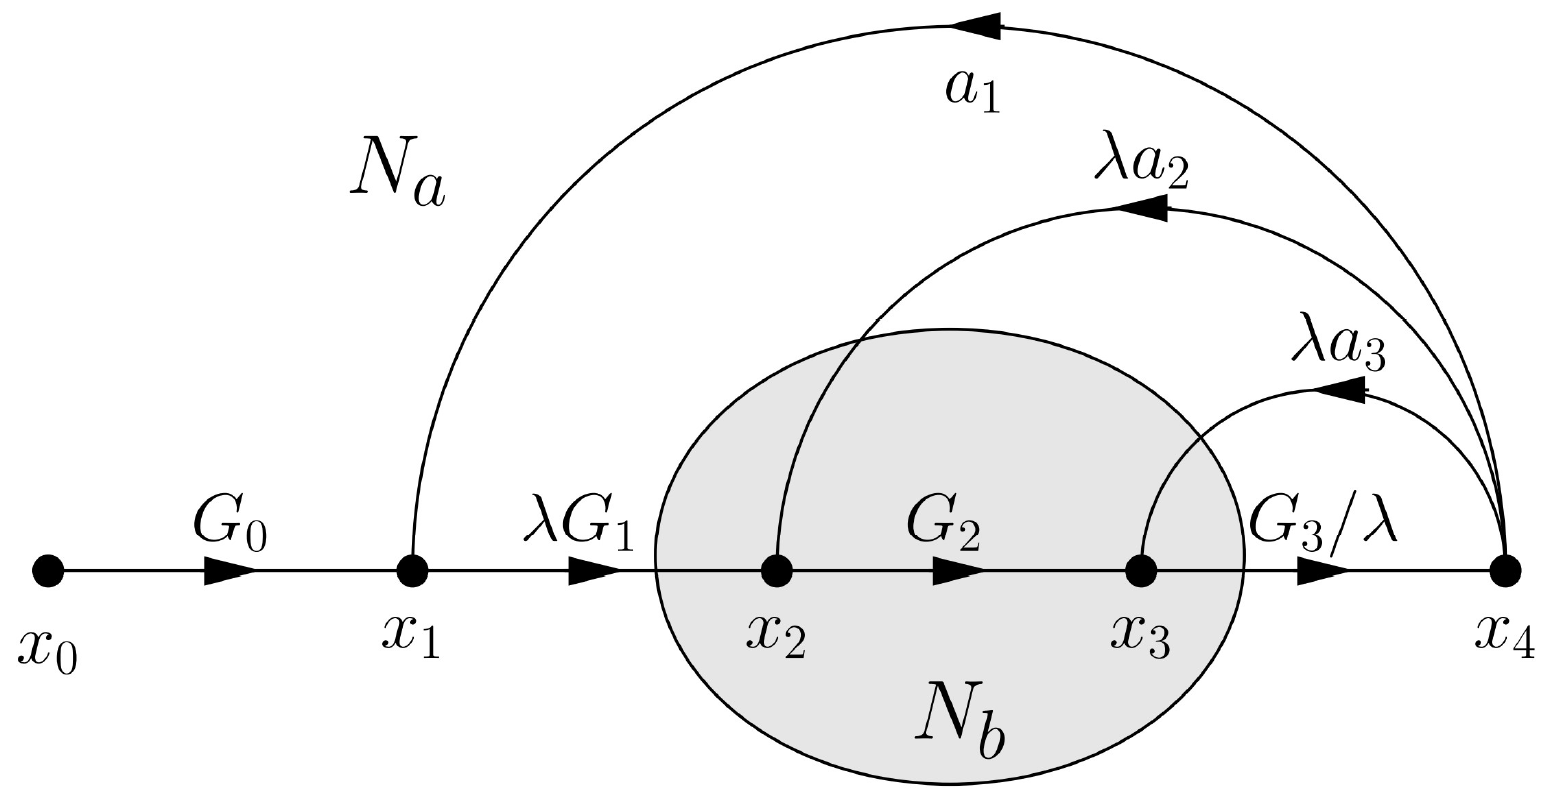
\includegraphics[width=\columnwidth]{images/skalierung.png}
\end{minipage}
\hfill
\begin{minipage}{0.44\columnwidth}
    \raggedright
\textbf{Eine Skalierung ändert die UTF und die Netzwerk-determinante $\bm{\Delta}$ nicht!}
\end{minipage}


\subsection{Anwendung: Operationsverstärker}{78-79}

\begin{center}
    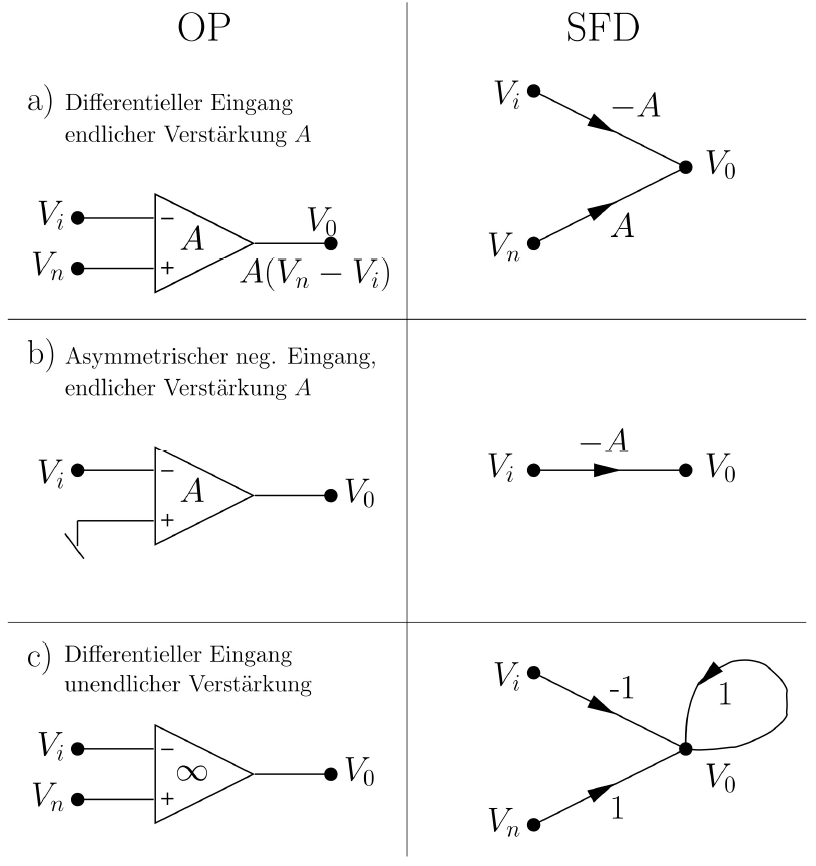
\includegraphics[width=0.7\columnwidth]{images/OPV_als_DFD.png}
\end{center}


		\section{Frequenzanalyse}{107}

\subsubsection{Bestimmung Frequenzspektrum pro Signalkategorie}

\begin{tabular}{l c l}
    \textbf{Periodische} Leistungssignale   & \textrightarrow\ & Fourier-Reihe              \\
    Energiesignale                          & \textrightarrow\ & Fourier-Transformation     \\
    Aperiodische Leistungssignale           & \textrightarrow\ & AKF \& Leistungsspektrum 
\end{tabular}


\subsubsection{Periodizität}

Ein periodisches Signal $a(t)$ \textbf{behält} durch Addition oder Subtraktion eines Signals $b(t)$ 
\textbf{gleicher Periode $\bm{T}$ (oder eines Teilers von $\bm{T}$) seine Periodizität} 
$$ c(t + T) = a(t + T) \pm b(t + T) = a(t) \pm b(t) = c(t) $$


\subsubsection{Orthogonalitätsrelationen Trigo-Funktionen}{109}

Die Orthogonalitätsrelationen können bei der Berechnung der Fourier-Reihen hilfreich sein.

\vspace{0.2cm}

\begin{tabular}{ll}
	$\int \limits_{0}^{T} \cos(m \, \omega_f \, t) \cdot \cos(n \, \omega_f \, t) \, \diff t = 
    \begin{cases}
    T,              & m = n = 0 \\
    \frac{T}{2},    & m = n > 0 \\
    0,              & m \neq n
    \end{cases} $ 
    & $(m, \; n \in \mathbb{N}_0)$ \\
    \\
    $\int \limits_{0}^{T} \sin(m \, \omega_f \, t) \cdot \sin(n \, \omega_f \, t) \, \diff t =      		
	\begin{cases}
    \frac{T}{2},    & m = n  \\
    0,              & m \neq n
    \end{cases} $ 
    & $(m, \; n \in \mathbb{N})$ \\
    \\
    $\int \limits_{0}^{T} \cos(m \, \omega_f \, t) \cdot \sin(n \, \omega_f \, t) \, \diff t = 0 $ 	
    & $(m \in \mathbb{N}_0, \; n \in \mathbb{N})$ 
\end{tabular}
	
\vspace{0.2cm}

$$ \sin(\alpha \pm \beta) = \sin(\alpha) \cdot \cos(\beta) \pm \cos(\alpha) \cdot \sin(\beta) $$
	

\subsection{Fourier-Reihe -- Trigonometrische Darstellung}{108}

Ist $f(t)$ eine \textbf{eindeutige}, reelle, stückweise \textbf{monotone} und \textbf{differenzierbare, periodische Funktion} mit der
\textbf{Primitivperiode $T$}, so lässt sich eine \textbf{Fourier-Reihe} von $f(t)$ entwickeln.

$$ \boxed{ f(t) \rightsquigarrow \frac{a_0}{2} + \sum\limits_{k=1}^\infty \Bigg( a_k\, \cos \Big(\frac{2 \, \pi \, k}{T} \, t \Big) + b_k\, \sin \Big(\frac{2 \, \pi \, k}{T} \, t \Big)  \Bigg) } $$

\textbf{$\bm{\frac{a_0}{2}}$ entspricht dem Mittelwert (Gleichstromanteil) der Funktion $\bm{f(t)}$ auf dem Intervall [$\bm{0}$ ; $\bm{T}$)} 


\subsubsection{Berechnung der Fourier-Koeffizienten}
\label{Berechnung der Fourier-Koeffizienten - Trigonometrisch}

$$ a_0 = \frac{2}{T} \cdot \int \limits_{0}^{T} f(t) \, \diff t $$
$$ a_k = \frac{2}{T} \cdot \int \limits_{0}^{T} f(t) \cdot \cos \Big( \frac{2 \, \pi \, k}{T} \, t \Big) \, \diff t \quad \text{ für } k \in N_0 $$
$$ b_k = \frac{2}{T} \cdot \int \limits_{0}^{T} f(t) \cdot \sin \Big( \frac{2 \, \pi \, k}{T} \, t \Big) \, \diff t \quad \text{ für } k \in N $$

\textbf{\crd{ \textrightarrow\ Trigo-Produkte in Integralen in SUMMEN umwandeln!!}}


\subsection{Fourier-Reihe - Harmonische Darstellung}{113}

Statt mit Sinus- und Cosinus-funktionen kann die Fourier-Reihe auch nach Betrag und Phase (Periode $T$) dargestellt werden:

$$  \boxed{ f(t) \rightsquigarrow \frac{a_0}{2} + \sum\limits_{k=1}^\infty \Big( d_k\, \cos \big(\frac{2 \, \pi \, k}{T} \, t + \phi_k \big) \Big) } $$

\begin{minipage}[c]{0.48\columnwidth}
    $$ \text{Betrag:} \quad d_k = \sqrt{a_k^2 + b_k^2} $$
\end{minipage}
\hfill
\begin{minipage}[c]{0.48\columnwidth}
    $$ \text{Phase:} \quad \phi_k = -\arctan \big( \frac{b_k}{a_k} \big) + n \, \pi $$ 
\end{minipage}


\subsubsection{Berechnung der Fourier-Koeffizienten}

\textrightarrow\ Berechnung von $a_k$ und $b_k$ gemäss Abschnitt ~\ref{Berechnung der Fourier-Koeffizienten - Trigonometrisch} \\
\textrightarrow\ Umrechung in Betrag und Phase

	
\subsection{Fourier-Reihe -- Komplexe Darstellung}{114}

Ausgehend von der \textbf{Eulerschen Formeln} kann man die Fourier-Reihe mit \textbf{Exponentialfunktionen} anstelle von Winkelfunktionen formulieren

\vspace{0.2cm}

\begin{minipage}{0.48\columnwidth}
    $$ \sin(t) = \frac{\e^{\jimg t} - \e^{- \jimg t}}{2j} $$ 
\end{minipage}
\hfill
\begin{minipage}{0.48\columnwidth}
    $$ \cos(t) = \frac{\e^{\jimg t} + \e^{- \jimg t}}{2} $$
\end{minipage}

\vspace{0.2cm}

$$  \boxed{ f(t) \rightsquigarrow \sum\limits_{k=-\infty}^\infty c_k \, e^{\jimg \frac{2 \, \pi \, k \, t}{T}} } $$


\subsubsection{Berechnung der komplexen Fourier-Koeffizienten $\bm{c_k}$}

\vspace{-0.2cm}

$$c_k = \overline{c_{-k}} = \frac{1}{T} \int\limits_0^T f(t) \cdot e^{- \jimg \frac{2 \, \pi \, k \, t}{T}}   \, \diff t =
\begin{cases}
\frac{a_0}{2}                       & \text{für } k = 0 \\
\frac{1}{2} (a_k - \jimg \, b_k)        & \text{für } k > 0 \\
\frac{1}{2} (a_{-k} + \jimg \, b_{-k})  & \text{für } k < 0
\end{cases} $$

$$ \text{Es gilt:} \quad a_k = c_k + c_{-k} \text{ und } b_k = \jimg (c_k - c_{-k}) $$ 

		
\subsection{Umrechnung der Fourier-Koeffizienten}

\renewcommand{\arraystretch}{1.5}
\begin{tabular}{ll}
    $c_k = \overline{c_{-k}} = \frac{a_k - \jimg \, b_k }{2}$   & ($k = 0, \, 1, \,  2\, \ldots \, ,$ wobei $b_0 = 0$)  \\
    $a_k = 2 \, \RE(c_k) = c_k + c_{-k}$                        & ($k = 0, \, 1, \,  2\, \ldots$)                       \\
    $b_k = -2 \, \IM(c_k) = \jimg(c_k - c_{-k})$                & ($k = 1, \,  2\, \ldots$)                             \\
    $d_k = 2 \, |c_k| = \sqrt{a_k^2 + b_k^2}$                   & $\phi_k = - \arctan \Big( \frac{b_k}{a_k} \Big)$
\end{tabular}
\renewcommand{\arraystretch}{1}
		
		
\subsection{Tipps zur Berechnung der Koeffizienten}{115}

\subsubsection{Achsensymmetrien}

\begin{center}
    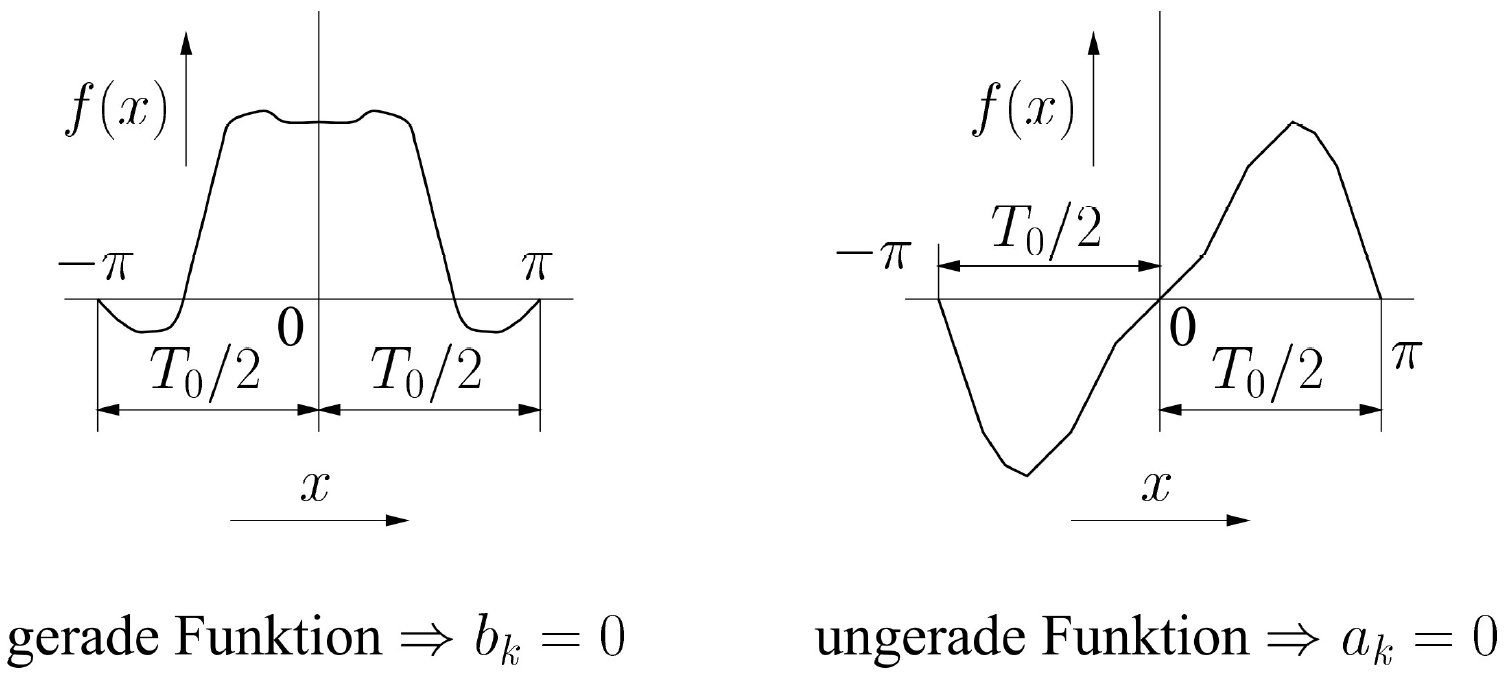
\includegraphics[width=0.75\columnwidth]{images/achsensymmetrie.png}

    \vspace{0.2cm}

    \begin{tabular}{lll}
        $f(t)$ gerade   & $a_k = \frac{4}{T} \cdot \int \limits_{0}^{\frac{T}{2}} f(t) \cdot \cos \Big( \frac{2 \pi k}{T} t \Big) \, \diff t$   & $b_k = 0$ \\
        \\
        $f(t)$ ungerade & $b_k = \frac{4}{T} \cdot \int \limits_{0}^{\frac{T}{2}} f(t) \cdot \sin \Big( \frac{2 \pi k}{T}  t \Big) \, \diff t$  & $a_k = 0$
    \end{tabular}
\end{center}	
		
\subsubsection{Symmetrie der Halbperioden}

Haben die Halbperioden die \textbf{gleiche Form} und sind in der \textbf{gleichen Lage zur x-Achse}, also $f(t) = f(t + \frac{T}{2})$,
so gibt es nur Glieder mit \textbf{geraden Argumenten}.

\vspace{0.2cm}	

Ist aber nur die \textbf{Form gleich} und die \textbf{Lage zur $\bm{x}$-Achse verschieden}, also $f(t) = - f(t + \frac{T}{2})$, so gibt es 
nur Glieder mit \textbf{ungeraden Argumenten}.

\begin{center}
    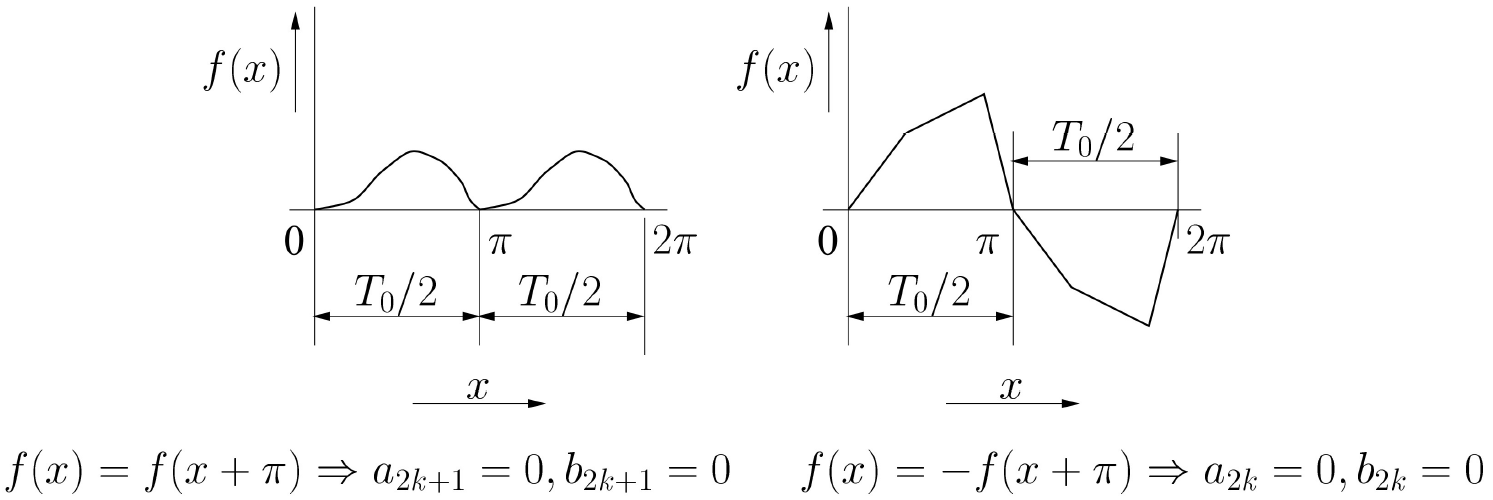
\includegraphics[width=0.9\columnwidth]{images/symmetrie_halbperioden.png}

    \vspace{0.2cm}

    \begin{tabular}{llll}
        links   & $a_{2k+1} = 0$    & $b_{2k+1} = 0$    & $a_0 \neq 0$ \\
        rechts  & $a_{2k} = 0$      & $b_{2k} = 0$      & $a_0 = 0$
    \end{tabular}
\end{center}


\subsection{Fourier-Koeffizienten und Leistung}{119}

Für den quadratischen Mittelwert $X^2$, also für die \textbf{Leistung} einer periodischen Funktion $x(t)$ gilt:

$$ \boxed{ X^2 = \sum\limits_{k=-\infty}^{\infty} |c_k|^2 = |c_0|^2 + 2 \, \sum\limits_{k=1}^{\infty} |c_k|^2 
    = \Big( \frac{a_0}{2} \Big)^2 + \sum\limits_{k=1}^{\infty} \frac{a_k^2 + b_k^2}{2} 
    = \Big( \frac{a_0}{2} \Big)^2 + \sum\limits_{k=1}^{\infty} \frac{d_k^2}{2} } $$		
		
		
\subsection{Gibbs'sches Phänomen}{112}

\begin{minipage}{0.35\columnwidth}
    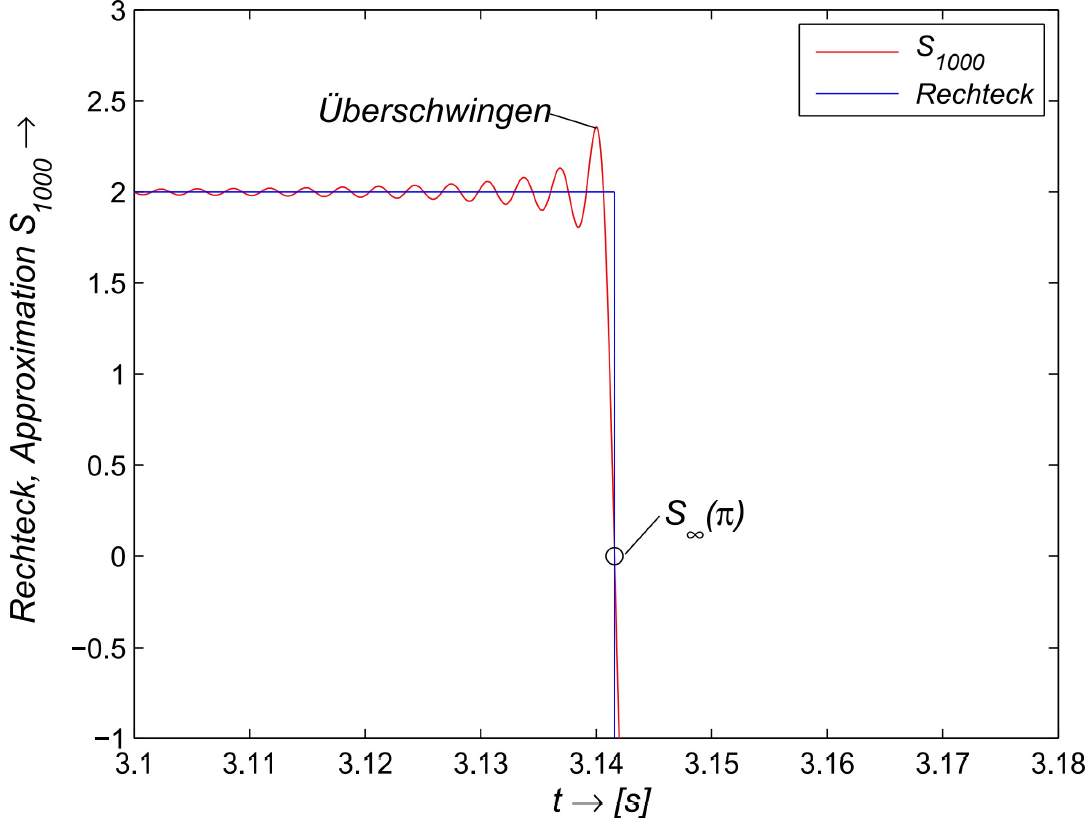
\includegraphics[width=\columnwidth]{images/gibbssches_phaenomen.png}
\end{minipage}
\hfill
\begin{minipage}{0.64\columnwidth}
    \raggedright
    An \textbf{Unstetigkeitsstellen} entsteht immer ein \textbf{Überschwingen}

    \vspace{0.2cm}

    \begin{itemize}
        \item ca. 18 \% der Amplitude ('peak')
        \item ca. 9 \% der Sprunghöhe ('peak-peak')
    \end{itemize}
\end{minipage}

\vspace{0.2cm}

Wenn $f(t)$ an der Stelle $t = t_0$ eine \textbf{Unstetigkeit} besitzt, dann ist die \textbf{Approximation} $S_{\infty}$ der 
Funktion $f(t)$ nicht nahe am richtigen Wert $f(t)$, egal wieviele Sinus- und Cosinus-Funktionen man verwendet.

$$ S_{\infty} = \frac{f(x_0^+) + f(x_0^-)}{2}  \quad \text{Mitte der Sprungstelle} $$

\columnbreak
		\section{Fourier-Transformation}{120}

Im Gegensatz zu den Fourier-Reihen, welche ausschliesslich periodische Signale 'verarbeiten' können, beschäftigt sich die 
Fourier-Transformation mit \textbf{nicht-periodischen Signalen!}


\subsection{Existenz des Fourier-Integrals}{131}

Die Fourier-Transformation von $f(t)$ und die inverse Fourier-Transformation existieren, wenn:

\subsubsection{Bedingung 1}

\vspace{-0.2cm}

$$ \boxed{ \int\limits_{- \infty}^{\infty} | f(t) | \, \diff t < \infty  \quad \text{ \textrightarrow\ \textbf{$\bm{f(t)}$ ist absolut integrierbar} }} $$

Diese Bedingung ist \textbf{hinreichend}, aber \textbf{nicht notwendig}!


\subsubsection{Bedingung 2}

$f(t)$ ist fouriertransformierbar, wenn:
$$ \boxed{ \int\limits_{- \infty}^{\infty} | F(\jimg \omega) | \, \diff \omega < \infty } $$

\textrightarrow\ \textbf{Die Fourier-Transformation $F(\jimg \omega)$ ist absolut integrierbar} 


\subsubsection{Bedingung 3}

$f(t)$ ist fouriertransformierbar, wenn:
\vspace{0.2cm}

\textbf{$\bm{f(t)}$ eine Linearkombination absolut integrierbarer Funktionen $\bm{f_i(t)}$ und inverser Fourier-Transformationen 
von $\bm{F_i(\jimg \omega)}$, die selber absolut integrierbar sind, ist.} 


\subsection{Berechnung der Fouriertransformation}{121}

\vspace{-0.2cm}	

$$ \boxed{ \text{Fouriertransformierte: \quad} F(\jimg \omega) = \int \limits_{-\infty}^{\infty} f(t) \, \e^{- \jimg \omega t} \, \diff t  } $$
$$ \boxed{ \text{Rücktransformation: \quad} f(t) = \frac{1}{2 \pi} \int \limits_{-\infty}^{\infty} F(\jimg \omega) \, \e^{\jimg \omega t} \, \diff \omega } $$		
		
$F(\jimg \omega)$ wird Fouriertransformierte oder \textbf{Spektralfunktion} genannt	


\subsubsection{Tipp: Berechnung von $\bm{F(0)}$}

\vspace{-0.2cm}	

$$ \boxed{ F(0) = \int \limits_{-\infty}^{\infty} f(t) \, \e^{- \jimg 0 t} \, \diff t =  \int \limits_{-\infty}^{\infty} f(t) \, \diff t } $$


\subsection{Konvergenzgeschwindigkeit}{122-123}

Je glatter eine Zeitfunktion $f(t)$ ist, desto schneller fällt ihre Fourier-Transformierte $F(\jimg \omega)$ ab und umgekehrt

% Idee: links und rechts von Hand Zeichnungen aus Vorlesungen dazumachen

\begin{center}
	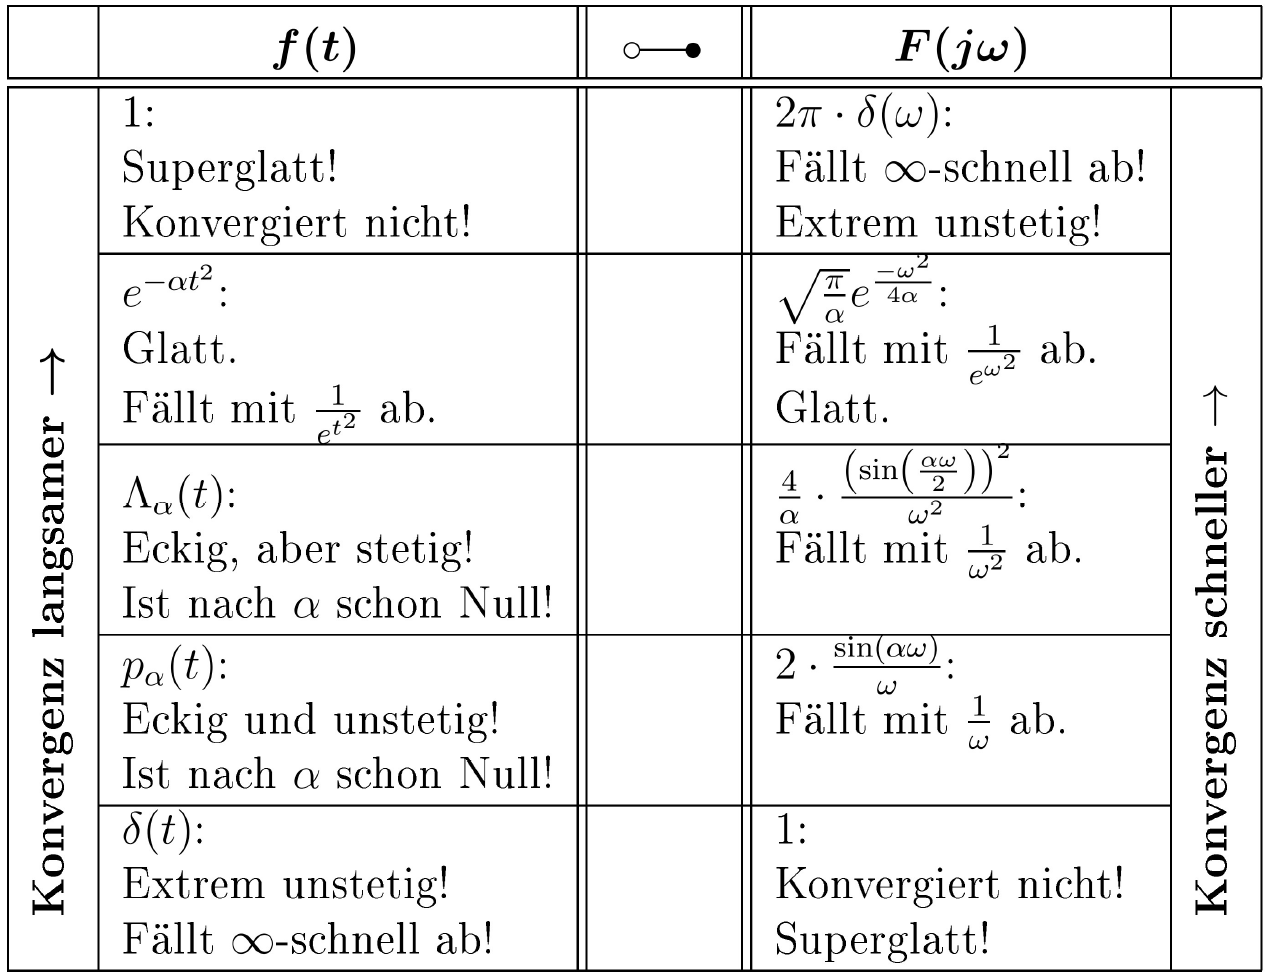
\includegraphics[width=0.7\columnwidth]{images/konvergenzgeschwindigkeit.png}
\end{center}

Im Frequenzbereich passiert das \textbf{duale} zum Zeitbereich!


\subsection{Eigenschaften der Fourier-Transformation}{124-130}

\subsubsection{Übersicht}

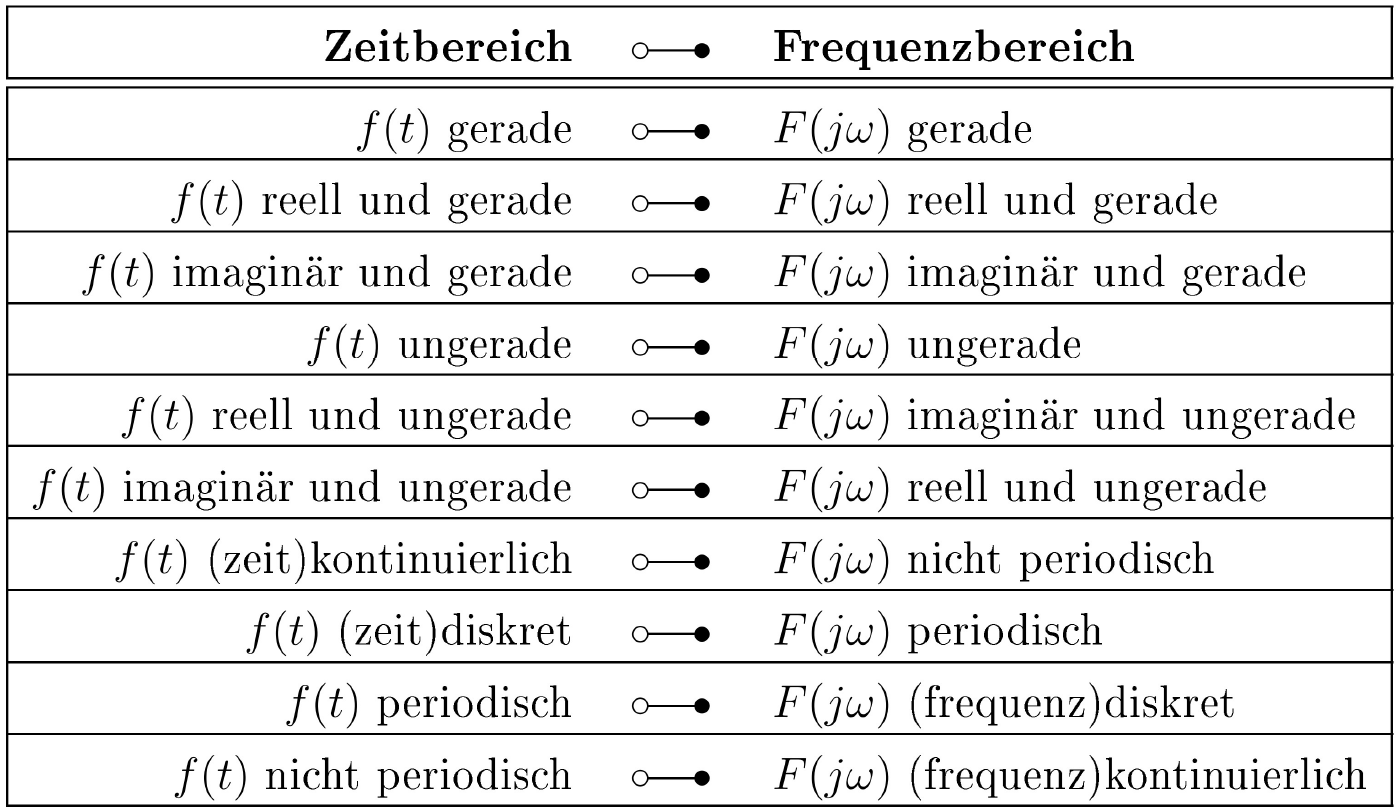
\includegraphics[width=\columnwidth]{images/eigenschaften_fourier_transformation}

\begin{center}
	\begin{tabular}{l c l}
		$f(t)$ reell 		& $\laplace$ 	& $F(-\jimg \omega) = F^*(\jimg \omega)$ konjugiert komplex	\\
		$f(-t) = f^*(t)$ 	& $\laplace$ 	& $F(\jimg \omega)$ reell
	\end{tabular}
\end{center}


\subsubsection{Linearität}

\vspace{-0.2cm}
$$ \boxed{ \alpha \cdot f(t) + \beta \cdot g(t) \, \laplace \, \alpha \cdot F(\jimg \omega) + \beta \cdot G(\jimg \omega)  \quad (\alpha, \, \beta \in \mathbb{C}) } $$


\subsubsection{Parseval's Theorem}

\vspace{-0.2cm}
$$ \boxed{ \int\limits_{- \infty}^{\infty} f(t) \, g^*(t) \, \diff t \, \laplace \, \frac{1}{2 \pi} \int\limits_{- \infty}^{\infty} F(\jimg \omega) \, G^*(\jimg \omega) \, \diff \omega } $$


\subsubsection{Bessel's Theorem (Rayleigh's Theorem)}

\vspace{-0.2cm}
$$ \boxed{ \int\limits_{- \infty}^{\infty} | f(t) | ^2 dt \, \laplace \, \frac{1}{2  \pi} \int\limits_{- \infty}^{\infty}  | F(\jimg \omega) |^2 \, \diff \omega } $$



\subsubsection{Ähnlichkeit (Streckung)}

\vspace{-0.2cm}
$$ \boxed{ f(\alpha \, t) \, \laplace \, \frac{1}{| \alpha |} F \Big( \jimg \, \frac{\omega}{\alpha} \Big) \quad \alpha \in \mathbb{R} \setminus \{ 0 \} } $$


\subsubsection{Verschiebung im Zeitbereich}

\vspace{-0.2cm}
$$ \boxed{ f( t \pm t_0 ) \, \laplace \, F(\jimg \omega) \, e^{\pm \jimg \omega t_0} } $$


\subsubsection{Verschiebung im Frequenzbereich}

\vspace{-0.2cm}
$$ \boxed{ f( t ) \, e^{\pm \jimg \omega_0 t} \, \laplace \, F(\jimg ( \omega \mp \omega_0 )) } $$


\subsubsection{Ableitung im Zeitbereich}

\vspace{-0.2cm}
$$ \boxed{ \frac{d^n f(t)}{d t^n}  \, \laplace \, (\jimg \omega)^n \, F(\jimg \omega) \quad n \in \mathbb{N}_0} $$


\subsubsection{Ableitung im Frequenzbereich}

\vspace{-0.2cm}
$$ \boxed{ t^n f(t) \, \laplace \, \jimg^n \frac{d^n F(\jimg \omega)}{d \omega^n} \quad n \in \mathbb{N}_0} $$


\subsubsection{Faltung im Zeitbereich (Multiplikation im Frequenzbereich)}

\vspace{-0.2cm}
$$ \boxed{ f(t)  * g(t) = \int\limits_{-\infty}^{\infty} f(\tau) \, g(t - \tau) \, d \tau \, \laplace \, F(\jimg \omega) \cdot G(\jimg \omega)  } $$


\subsubsection{Faltung im Frequenzbereich (Multiplikation im Zeitbereich)}

\vspace{-0.2cm}
$$ \boxed{ f(t) \cdot g(t) \, \laplace \, \frac{1}{2 \pi} F(\jimg \omega) * G(\jimg \omega) } $$

\subsubsection{Vertauschungssatz (Dualität)}

\vspace{0.2cm}

\begin{minipage}[c]{0.48\columnwidth}
	$$ \boxed{ f(t) \, \laplace \, F(\jimg \omega) } $$
\end{minipage}
\hfill
\begin{minipage}[c]{0.48\columnwidth}
	$$ \boxed{ F(\jimg t) \, \laplace \, 2 \pi \cdot f(- \omega) } $$
\end{minipage}


\subsubsection{Modulation}

\vspace{-0.2cm}
$$ \boxed{ \cos(\alpha t) \cdot f(t) \, \laplace \, \frac{1}{2} \cdot\Big[ F(\jimg ( \omega - \alpha)) + F(\jimg(\omega + \alpha)) \Big] } $$
$$ \boxed{ \sin(\alpha t) \cdot f(t) \, \laplace \, \frac{1}{2 \jimg} \cdot\Big[ F(\jimg ( \omega - \alpha)) - F(\jimg(\omega + \alpha)) \Big] } $$


\subsubsection{Zeitumkehrung}

\vspace{-0.2cm}
$$ \boxed{ f(-t) \, \laplace \, F(-\jimg \omega) } $$


\subsubsection{Integration im Zeitbereich}

\vspace{-0.2cm}
$$ \boxed{ \int\limits_{-\infty}^t  f(\tau) \, d \tau \, \laplace \, \frac{F(\jimg \omega)}{\jimg \omega} + F(\jimg0) \pi \delta(\omega) } $$


\subsubsection{Anfangswerte}

\vspace{-0.2cm}
$$ \boxed{ f(0) = \frac{1}{2 \pi}  \int\limits_{-\infty}^{\infty}  F(\jimg \omega) \, \diff \omega \qquad \qquad F(\jimg0) = \int\limits_{-\infty}^{\infty} f(t) \, \diff t } $$


\subsubsection{Unendlich lange Folge von Dirac-Pulsen}

\vspace{-0.2cm}
$$ \boxed{ \sum\limits_{n = -\infty}^{\infty}  \delta(t - n \cdot t_0) \, \laplace \,   \sum\limits_{n = -\infty}^{\infty} \frac{2 \pi}{t_0} \, \delta \Big( \omega - n \cdot \frac{2 \pi}{t_0} \Big)  } $$


\subsection{AKF und Leistungsdichtespektrum}{132}

\subsubsection{Leistungsdichtespektrum}

Die \textbf{normierte Leistung $\bm{P_n}$} eines \textbf{Leistungssignals $\bm{f(t)}$} kann mit der Hilfe des 
\textbf{Leistungsdichtespektrums $\bm{\Phi(\jimg \omega)}$} beschrieben werden.
$$ \boxed{  P_n = \lim\limits_{T \to \infty} \frac{1}{T} \int\limits_{-T/2}^{T/2} | f(t) |^2 \, \diff t
	= \frac{1}{2 \pi} \int\limits_{-\infty}^{\infty} \Big( \lim\limits_{T \to \infty} \frac{|F(\jimg \omega)|^2}{T} \Big) \, \diff \omega } $$

\vspace{0.2cm}

Der Integrand wird als \textbf{Leistungsdichtespektrums $\bm{\Phi(\jimg \omega)}$} bezeichnet:
$$ \boxed{ \Phi(\jimg \omega) = \lim\limits_{T \to \infty} \frac{|F(\jimg \omega) |^2}{T} } $$

\vspace{0.2cm}

Die \textbf{normierte Leisung $\bm{P_n}$} ist somit:
$$ \boxed{ X^2 = \varphi_{xx}(0) = P_n = \frac{1}{2 \pi}  \int\limits_{- \infty}^{\infty}  \Phi(\jimg \omega) \, \diff \omega } $$


\subsubsection{Energiedichtespektrum}
Analog zum Leistungsdichtespektrum lässt sich für ein \textbf{Energiesignal} (Klasse 1) das 
\textbf{Energiedichtespektrum $\bm{E(\jimg \omega)}$} finden
$$ \boxed{ W_n = \lim\limits_{T \to \infty} \int\limits_{-T/2}^{T/2} |f(t)|^2 \, \diff t = \frac{1}{2 \pi}  \int\limits_{- \infty}^{\infty} |F(\jimg \omega)|^2 \, d\omega } $$

\vspace{0.2cm}

Das \textbf{Energiedichtespektrum $\bm{E(\jimg \omega)}$} ist somit
$$ \boxed{ E(\jimg \omega) = |F(\jimg \omega)|^2 } $$


\subsection{Wiener-Chintschin Theorem}{133}

\subsubsection{Aperiodische Leistungssignale (Klasse 2b)}

Die AKF und das Leistungsdichtespektrum sind ein Fourier-Transformationspaar
$$ \boxed{ \varphi_{xx}(t) = \frac{1}{2 \pi} \int\limits_{- \infty}^{\infty} \Phi(\jimg \omega) \, e^{\jimg \omega t} \, d\omega \, \laplace \, \Phi(\jimg \omega) 
	= \int\limits_{- \infty}^{\infty} \varphi_{xx}(t) \, e^{-\jimg \omega t} \, \diff t } $$


\subsubsection{Periodische Leistungssignale (Klasse 2a) }

$$ \boxed{ \varphi_{xx}(t) = \sum\limits_{k = - \infty}^{\infty} |c_k|^2  \, e^{\jimg \frac{2 \pi k}{T_0} t } \, \laplace \, \Phi(\jimg \omega) 
	= 2 \pi \sum\limits_{k = - \infty}^{\infty}  |c_k|^2 \delta \Big( \omega - \frac{2 \pi k}{T_0} \Big) } $$


\subsubsection{Energiesignale (Klasse 1) }
Die AKF und das Energiedichtespektrum sind ein Fourier-Transformationspaar
$$ \boxed{ \varphi_{xx}(t) = \frac{1}{2 \pi} \int\limits_{- \infty}^{\infty} E(\jimg \omega) \, e^{\jimg \omega t} \, d\omega \, \laplace \, E(\jimg \omega)
	= \int\limits_{- \infty}^{\infty} \varphi_{xx}(t) \, e^{-\jimg \omega t} \, \diff t } $$

\columnbreak


		\section{Laplace-Transformation}{135}

Die Laplace-Transformation kann als analytische Fortsetzung der Fourier-Transformation aufgefasst werden. \\
Die Frequenz ist nun komplex $\cbl{(s = \sigma + \jimg \omega)}$ anstelle $\jimg \omega$. Dank dem Dämpfungsfaktor $\sigma$ kann die
Konvergenz von Signalen erzwungen werden.


\subsection{Berechnung der Laplace-Transformation}{135}
\label{Berechnung der Laplace-Transformation}

Komplexe Frequenz: $s = \sigma + \jimg \omega $

$$ \boxed{\text{Laplacetransformation: } F(s) = \int\limits_{0_-}^{\infty} f(t) \, e^{-st} \, \diff t  } $$
$$ \boxed{ \text{Rücktransformation: } f(t) = \frac{1}{2 \pi \jimg} \int\limits_{c - \jimg \infty}^{c+ \jimg \infty} F(s) \, e^{st} \, \diff s  } $$

\textrightarrow\ Für die Rücktransformation werden meistens Tabellen verwendet!


\subsection{Eigenschaften der Laplace-Transformation}{136-138}

\subsubsection{Linearität}

\vspace{-0.2cm}
$$ \boxed{ \alpha \cdot f(t) + \beta \cdot g(t) \, \laplace \, \alpha \cdot F(s) + \beta \cdot G(s)  \quad (\alpha, \, \beta \in \mathbb{C}) } $$


\subsubsection{Ähnlichkeit (Streckung)}

\vspace{-0.2cm}
$$ \boxed{ f(\alpha \, t) \, \laplace \, \frac{1}{| \alpha |} F \Big(\frac{s}{\alpha} \Big) \quad ( 0 < \alpha \in \mathbb{R}) } $$


\subsubsection{Faltung im Zeitbereich (Multiplikation im Frequenzbereich)}

\vspace{-0.2cm}
$$ \boxed{ f(t) * g(t) = \int\limits_{-\infty}^{\infty} f(\tau) \, g(t - \tau) \, \diff \tau 
    = \int\limits_{0}^{t} f(\tau) \, g(t - \tau) \, \diff \tau  \, \laplace \, F(s) \cdot G(s) } $$


\subsubsection{Faltung im Frequenzbereich (Multiplikation im Zeitbereich)}

\vspace{-0.2cm}
$$ \boxed{ f(t) \cdot g(t) \, \laplace \, \frac{1}{2 \pi \jimg} \int\limits_{c- \jimg \infty}^{c + \jimg \infty} F(\xi) \, G(s - \xi) \, \diff \xi } $$


\subsubsection{Ableitung(en) im Zeitbereich}

\renewcommand{\arraystretch}{1.5}
\begin{tabular}{r c l}
    $\frac{\diff f(t)}{\diff t}$        & $ \laplace$   & $s F(s) - f(0_-)$                                                                             \\
    $\frac{\diff^2 f(t)}{\diff t^2}$    & $\laplace$    & $s^2 F(s) - s f(0_-) - \frac{\diff f(0_-)}{\diff t}$                                          \\
    $\frac{\diff^3 f(t)}{\diff t^3}$    & $\laplace$    & $ s^3 F(s) - s^2 f(0_-) - s \frac{\diff f(0_-)}{\diff t} -\frac{\diff ^2f(0_-)}{\diff t^2}$   \\
                                        & \vdots        &                                                                                               \\
    $\frac{\diff^n f(t)}{\diff t^n}$    & $\laplace$    & $s^n F(s) - s^{n-1} f(0_-) - s^{n-2} \frac{\diff f(0_-)}{\diff t} - \ldots - \frac{\diff^{n-1} f(0_-)}{\diff t^{n-1}}$
\end{tabular}
\renewcommand{\arraystretch}{1}


\subsubsection{Multiplikation mit $\bm{t}$}

\vspace{-0.2cm}
$$ \boxed{ t \cdot f(t) \, \laplace \, - \frac{\diff F(s)}{\diff s} } $$



\subsubsection{Ableitung im Frequenzbereich}

\vspace{-0.2cm}
$$ \boxed{ (-t)^n f(t) \, \laplace \,  \frac{\diff ^n F(s)}{\diff s^n} \qquad (n \in \mathbb{N}_0) } $$


\subsubsection{Verschiebung im Zeitbereich}

\begin{minipage}[c]{0.48\columnwidth}
    $$ \boxed{ f( t \pm t_0 ) \, \laplace \, F(s) \, e^{\pm t_0 s} } $$
\end{minipage}
\hfill
\begin{minipage}[c]{0.48\columnwidth}
    \begin{tabular}{ll}
        Minus:  & wenn $t_0 > 0$                \\
        Plus:   & wenn $f(t) = 0$ für $t < t_0$
    \end{tabular}
\end{minipage}


\subsubsection{Verschiebung im Frequenzbereich (Dämpfung im Zeitbereich)}

\vspace{-0.2cm}
$$ \boxed{ f( t ) \, e^{\mp \alpha t} \, \laplace \, F(s \pm \alpha ) } $$


\subsubsection{Integration im Zeitbereich}

\vspace{-0.2cm}
$$ \boxed{ \int\limits_0^t  f(\tau) \, \diff \tau \, \laplace \, \frac{F(s)}{s} } $$


\subsubsection{Grenzwertsätze}

\vspace{-0.4cm}
\begin{align*}
    \text{\textbf{Anfangswert:}}    & \qquad \boxed{ \lim\limits_{t \to 0} f(t) = \lim\limits_{s \to \infty} s F(s) \quad \text{wenn } \lim\limits_{t \to 0} f(t) \text{ existiert} } \\
    \text{\textbf{Endwert:}}        & \qquad \boxed{ \lim\limits_{t \to \infty} f(t) = \lim\limits_{s \to 0} s F(s) \quad \text{wenn } \lim\limits_{t \to \infty} f(t) \text{ existiert (Pole von } sF(s) \text{ in der linken Halbebene)} }
\end{align*}


\subsubsection{Weitere Zusammenhänge und Tabellen}

\textrightarrow\ Siehe Skript Anhang 3.B


\subsection{Rücktransformation in den Zeitbereich }{139-141}

\textbf{\textrightarrow\ Meistens werden Tabellen verwendet!}


\subsubsection{Rücktransformation mittels Umkehrintegral}

\textrightarrow\ Siehe Abschnitt \ref{Berechnung der Laplace-Transformation}


\subsubsection{Rücktransformation gebrochen-rationaler Funktionen (PBZ)}

\myul{\textbf{Vorgehen Partialbruchzerlegung}}

\vspace{0.1cm}

\begin{enumerate}
  \item Nennerpolynom faktorisieren
  \item Bruch als Summe aus Faktoren schreiben
  \item Gleichsetzen mit ursprünglichem Term
  \item Koeffizientenvergleich (Zähler finden)
  \item Rücktransformation der einzelnen Summanden mit Tabellen
\end{enumerate}


\subsubsection{Rücktransformation mittels Residuensatz}

\textbf{ \textrightarrow\ Empfohlen für PBZ mit mehreren Polen}

$$ \boxed{ A_{ij} = \frac{1}{(n_i - j)!} \frac{\partial^{n_i - j}}{\partial s^{n_i-j}} \big[ (s-p_i)^{n_i} F(s) \big] \Bigg|_{s = p_i} } $$


\example{Residuensatz}

$$\text{Gegeben:} \quad  F(s) = Y(s) = \sum\limits_{i=1}^k  \sum\limits_{j=1}^{n_k} \frac{A_{ij}}{(s-p_i)^j} = \frac{6}{(s+4) \cdot (s+3)^2} $$
$$ \text{Ansatz PBZ:} \quad \frac{A_{11}}{s+4} + \frac{A_{21}}{s+3} + \frac{A_{22}}{(s+3)^2} $$

\begin{align*}
    A_{11}  &= \frac{1}{0!} \frac{\partial^0}{\partial s^0} (s+4) \cdot \frac{6}{(s+4) \cdot (s+3)^2} \Big|_{s = -4} = \frac{6}{(s+3)^2} \Big|_{s = -4} = 6 \\
    A_{21}  &= \frac{1}{1!} \frac{\partial}{\partial s} (s+3)^2 \cdot \frac{6}{(s+4) \cdot (s+3)^2} \Big|_{s = -3} =  \frac{\partial}{\partial s} \frac{6}{s+4} \Big|_{s = -3} = \frac{-6}{(s+4)^2} \Big|_{s = -3} = -6 \\
    A_{22}  &= \frac{1}{0!} \frac{\partial^0}{\partial s^0} (s+3)^2 \cdot \frac{6}{(s+4) \cdot (s+3)^2} \Big|_{s = -3} = 6
\end{align*}


% Von Zusammenfassung Integraltransformationen:
\subsection{Lineare DGL mittels Laplacetransformation lösen}
		
\subsubsection{Vorgehen: Lösen einer DGL mit Laplace}
		
\begin{enumerate}
    \item DGL inkl. Störfunktion $f(t)$ in Bildbereich transformieren \\
        \textrightarrow\ Anfangswerte für $f^{(n)}(0_-)$ einsetzen!
    \item Gleichung nach Laplace-Transofrmierter der gesuchten Funktion umformen
    \item Rücktransformation in den Zeitbereich
\end{enumerate}

		
\example{Lösung einer DGL mit Laplace}

\begin{minipage}[c]{0.6\columnwidth}
    \begin{tabular}{ll}
        DGL:            & $\ddot{y}(t) + 2 \, \dot{y}(t) + 5 \, y(t) = f(t)$ \\
        Anfangswerte:   & $y(0) = 0$; \quad $\dot{y}(0) = 0$
    \end{tabular}
\end{minipage}
\hfill
\begin{minipage}[c]{0.35\columnwidth}
    \textrightarrow\ Finde $y(t)$
\end{minipage}

\vspace{0.2cm}

\begin{enumerate}
    \setlength\itemsep{3pt}
    \item $\laplace \; s^2 \cdot Y(s) - s \cdot 0 - 0 + 2( s \cdot Y(s) - 0) + 5 \cdot Y(s) = 1(s)$ \\
        $s^2 \cdot Y(s)+ 2 \cdot s \cdot Y(s) + 5 \cdot Y(s) = 1(s)$
    \item $Y(s) = \frac{1}{s^2 + 2s +5}$
    \item Rücktransformation mit Tabellen
\end{enumerate}


% Aus Integraltransformationen
\subsection{Konvergenzhalbebene}
\label{Konvergenzhalbebene}

Es gibt jeweils mehrere (komplexe) Zahlen $s$, \textbf{für welche das Laplace-Integral konvergiert.} 
Die Konvergenzhalbebene beinhaltet alle diese Zahlen $s$

\vspace{0.2cm}

\begin{minipage}[c]{0.48\columnwidth}
    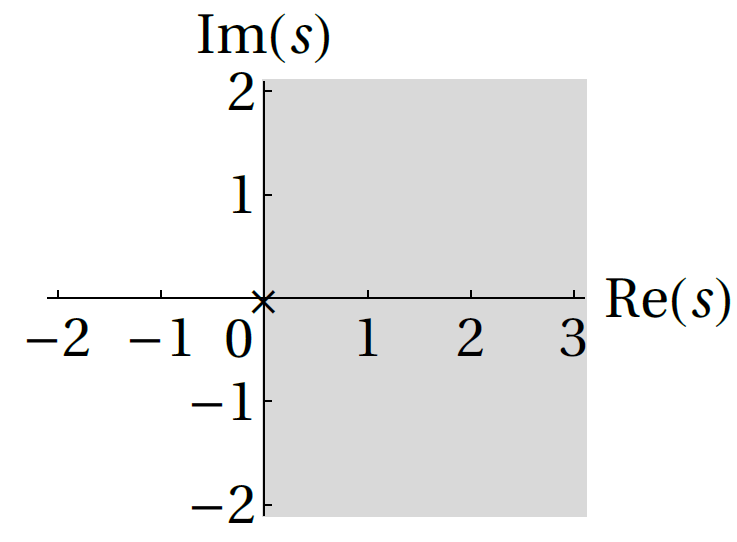
\includegraphics[width=\columnwidth]{images/konvergenzhalbebene.png} 
\end{minipage}
\hfill
\begin{minipage}[c]{0.48\columnwidth}
    Die Halbebene wird durch die \textbf{am weitesten rechts liegende Polstelle} von $F(s)$ begrenzt (Kreuzchen)
    \vspace{0.2cm}
    Falls $F(s)$ keine Polstelle hat, ist die Konvergenzhalbebene gleich $\mathbb{C}$
\end{minipage}


\subsection{Zusammenhang LT und FT}{145}

Bei kausalen, stabilen und fourier-transformierbaren Signalen $f(t)$ kann man durch das Ersetzen von $s = \sigma + \jimg \omega$ 
durch $\jimg \omega$ (und umgekehrt) zwischen der einseitigen Laplace-Transformation und der Fourier-Transformation wechseln.

\vspace{0.2cm}

Kennt man die einseitige Laplace-Transformation $F(s)$ des kausalen Signals $f(t)$, so kann man folgende Aussagen machen:

\vspace{0.1cm}

\begin{itemize}
    \setlength\itemsep{3pt}
    \item Liegt die $\jimg \omega$-Achse im Konvergenzbereich von $F(s)$, so kann $s$ 
        durch $\jimg \omega$ ausgetauscht werden, um $F(\jimg \omega)$ zu erhalten. 
    \item Liegt die $\jimg \omega$-Achse ausserhalb des Konvergenzbereichs von 
        $F(s)$, so konvergiert die Fourier-Transformation $F(\jimg \omega)$ nicht.
    \item Liegt die $\jimg \omega$-Achse auf dem Rand des Konvergenzbereichs von
        $F(s)$, so \textbf{können} die Fourier-Transformation $F(\jimg \omega)$ und die
        einseitige Laplace-Transformation $F(s)$ übereinstimmen, \textbf{müssen aber nicht}.
\end{itemize}

		\section{Systembeschreibung}{161}

Ein System transformiert mindestens ein Eingangssignal $x(t)$ in mindestens ein Ausgangssignal $y(t)$.
Die Zuordnung zwischen Eingang und Ausgang muss \textbf{eindeutig} sein! \\
Die Transformation erfolgt mittels Übertragungsfunktion $H(s)$ (UTF)

\vspace{-0.6cm}

\begin{center}
    $$ \boxed{H(s) = \frac{Y(s)}{X(s)}} $$
    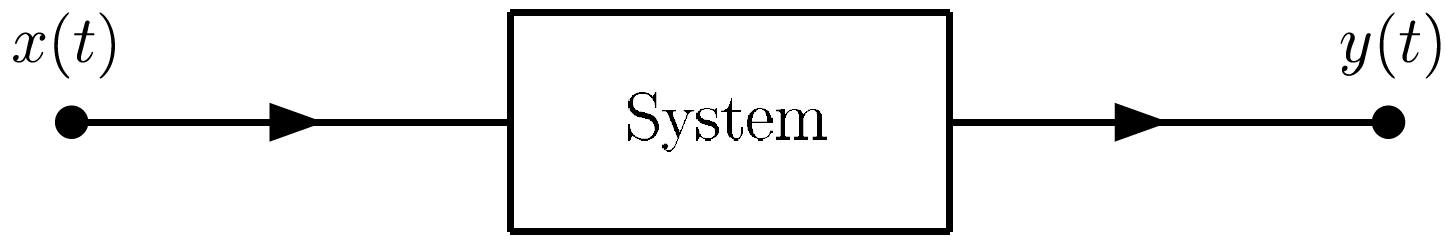
\includegraphics[width=0.75\columnwidth]{images/system.png}
\end{center}


\subsection{Eingangs-zu-Ausgangsbeziehungen }{161}

\begin{tabular}{ll}
    SISO & Single Input Single Output       \\
    MIMO & Multiple Input Multiple Output   \\
    MISO & Multiple Input Single Output 
\end{tabular}


\subsubsection{Wirkungsfreiheit}{161-162}

\begin{itemize}
    \item Systemausgänge dürfen nachfolgende Systeme nicht beeinflussen
    \item Systemeingänge dürfen vorhergehende Systeme nicht beeinflussen
\end{itemize}

\vspace{-0.2cm}

\begin{center}
    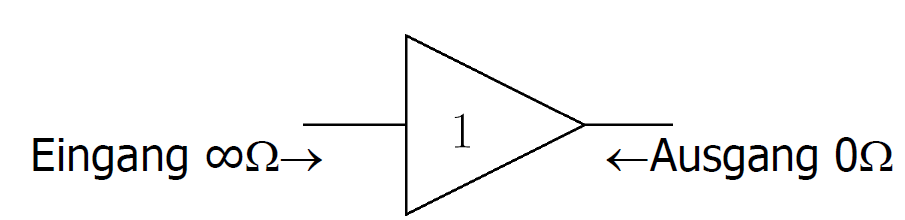
\includegraphics[width=0.7\columnwidth]{images/wirkungsfreiheit.png}
\end{center}


\subsection{Invertierbare vs. nichtinvertierbare System}{173}

\subsubsection{Invertierbare Systeme}

Ein System wird als \textbf{invertierbar} bezeichnet, wenn bei jedem Ausgangssignal \textbf{eindeutig} auf das entsprechende 
Eingangssignal geschlossen werden kann.

\vspace{0.2cm}

\example{(Nicht) Invertierbare Systeme}

\begin{minipage}[t]{0.48\columnwidth}
    $y = x^2$ \quad \textrightarrow\ nicht invertierbar
\end{minipage}
\hfill
\begin{minipage}[t]{0.48\columnwidth}
    $y = x^3$ \quad \textrightarrow\ invertierbar 
\end{minipage}


\subsection{Reelle Systeme vs. komplexwertige Systeme}{173}

Ein System wird als \textbf{reell} bezeichnet, wenn ein \textbf{relles Eingangssignal} immer ein \textbf{reelles Ausgangssignal} bewirkt.


\subsection{Statische vs. Dynamische Systeme}{162-163}

\subsubsection{Statische (resistive) Systeme (System ohne Gedächtnis)}


Der Wert des Ausgangssignals $y(t_0)$ zum gegenwärtigen Zeitpunkt $t_0$ \textbf{hängt nur vom gegenwärtigen Wert des Eingangs $\bm{x(t_0)}$ ab}. \\
Systembeschreibung: algebraische Gleichungen 
$$ \boxed{ y(t_0) = f\{x(t_0) \} \, \forall \, t_0  } $$


\subsubsection{Dynamische Systeme (System mit Gedächtnis)}

Der Wert des Ausgangssignals $y(t_0)$ zum gegenwärtigen Zeitpunkt $t_0$ \textbf{hängt auch von anderen Zeitpunkten als $\bm{t = t_0}$ ab}. \\
In elektrischen Systemen wirken $L$ und $C$ als Speicherelemente und machen ein System dynamisch. \\
Systembeschreibung: Differentialgleichungen


\subsection{Kausale vs. akausale Systeme}{164}

\begin{itemize}
    \item \textbf{Alle statischen} Systeme sind \textbf{kausal} 
    \item \textbf{Nicht alle kausalen} Systeme sind \textbf{statisch}
\end{itemize}



\subsubsection{Kausale Systeme}

Der Wert des Ausgangssignals $y(t_0)$ hängt nur von Eingangssignalen $x(t \leq t_0)$ ab. \\
\textrightarrow\ 'Das System kann \textbf{nicht} in die Zukunft schauen' \\
\vspace{0.1cm}
\crd{\textbf{Physikalische Systeme sind immer kausale Systeme!}}


\subsubsection{Akausale Systeme}

Der Wert des Ausgangssignals $y(t_0)$ hängt auch von \textbf{zukünftigen} Eingangsignalen $x(t > t_0)$ ab. \\
\textrightarrow\ 'Das System sieht in die Zukunft' 


\subsection{Lineare vs. nichtlineare Systeme}{165-166}

\subsubsection{Lineare Systeme}

Bei einem linearen System gilt das \textbf{Superpositionsprinzip} 
$$ \boxed{   f\{a \cdot x_1(t) + b \cdot x_2(t) \} = a \cdot f \{ x_1(t)   \} + b \cdot f \{ x_2(t) \} } $$

\textbf{\textrightarrow\ Alle Systeme, die nur als $\bm{R}$, $\bm{L}$ und $\bm{C}$ bestehen, sind linear.} 

\vspace{0.2cm}

Alle Differentialgleichungen der Form
$$ \boxed{ \sum\limits_{i=0}^n  a_i \frac{\diff^i y(t) }{\diff t^i} = \sum\limits_{j=0}^m  b_j \frac{\diff^j x(t) }{\diff t^j} \, \laplace \, Y(s) \cdot \sum\limits_{i=0}^n a_i s^i = X(s) \cdot \sum\limits_{j=0}^m b_j s^j } $$
beschreiben ein lineares, kausales, zeitinvariantes System (LTI-System), sofern $m \leq n$. Die Laplace-Korrespondenz gilt für Anfangswerte $= 0$.


\subsubsection{Nichtlineare Systeme}{167}

Ein System, welches bei \textbf{kurzgeschlossenem Eingang} ($x(t) = 0$) ein \textbf{Ausgangssignal} hat ($y(t) \neq 0$), 
ist \textbf{sicher nichtlinear} (hinreichend, nicht notwendig: z.B. $y = x^2$ ist nichtlinear mit $y(0) = 0$).

\vspace{0.1cm}

\textrightarrow\  Nichtlineare Systeme erlauben das Erzeugen \textbf{neuer Frequenzanteile}.

\vspace{0.2cm}
\myul{\textbf{Beispiel:}}

\vspace{0.1cm}
Gerade, welche nicht durch Ursprung geht


\subsection{Zeitinvariante vs. zeitvariante Systeme}{170}

\subsubsection{Zeitinvariante Systeme}

Ein System ist \textbf{in}variant, wenn eine zeitliche Verschiebung des Eingangssignals $x(t)$ um eine feste Zeit $t_0$ 
eine \textbf{gleich grosse Zeitverschiebung am Ausgang} bewirkt aber die Form des Signals nicht ändert.

$$ \boxed{ x(t) \to y(t), \text{ dann gilt } x(t- t_0) \to y(t- t_0) \, \forall \, t_0  } $$

Trifft dies nicht zu, so handelt es sich um ein \textbf{zeitvariantes} System.


\subsubsection{Zusammenhänge bei statischen Systemen}{170}

\begin{center}
    \begin{tabular}{lll}
        \toprule
        \textbf{Zusammenhang}                   & \textbf{Mathemetische Darstellung}        & \textbf{Beispiel}         \\
        \midrule
        linear \& zeit\textbf{in}variant        & $y(t) = \gamma \cdot x(t)$                & $y(t) = 3 \cdot x(t)$     \\
        \midrule
        linear \& zeitvariant                   & $y(t) = \gamma(t) \cdot x(t)$             & $y(t) = t^2 \cdot x(t)$   \\
        \midrule
        nichtlinear \& zeit\textbf{in}variant   & $y(t) = f\{x(t)\}$                        & $y(t) = 4 \cdot x^2(t)$   \\
        \midrule
        nichtlinear \& zeitvariant              & $y(t) = f\{x(t), \, t\}$                  & $y(t) = t \cdot x^3(t)$   \\
        \bottomrule
    \end{tabular}
\end{center}


		\section{LTI-Systeme}{171}

\begin{tabular}{ll}
	$x(t)$ 				& Eingangssignal 										\\
	$y(t)$ 				& Ausgangssignal 										\\
	$\delta(t)$ 		& Dirac-Stoss 											\\
	$h(t)$ 				& Impulsantwort (Antwort auf Dirac-Stoss) 				\\
	$H(\jimg \omega)$ 	& Frequenzgang 											\\
	$H(s)$ 				& $H(s) = \frac{Y(s)}{X(s)}$ Übertragungsfunktion (UTF)
\end{tabular}


\subsection[Bestimmung des Ausgangssignals]{Bestimmung des Ausgangssignals $\bm{y(t)}$}{173}

Das Ausgangssignal $y(t)$ eines Systems entspricht der \textbf{Faltung} des Eingangssignals $x(t)$ mit der Impulsantwort $h(t)$ des Systems.
$$ \boxed{ y(t) = \int\limits_{-\infty}^{\infty} x(\tau) h(t-\tau) \, \diff \tau = \int\limits_{-\infty}^{\infty} h(\tau) x(t-\tau) \, \diff \tau } $$

Die Faltungsoperation kann auch mit dem \textbf{Stern-Operator} geschrieben werden:
$$ \boxed{ y(t) = x(t) * h(t) = h(t) * x(t) = (x * h)(t) } $$

\vspace{0.2cm}

Im Bildbereich bestimmt man die Fourier-Transformierte der Ausgangsfunktion als:
$$ \boxed{ Y(\jimg \omega) = H(\jimg \omega) \cdot X(\jimg \omega) } \qquad \text{mit } H(\jimg \omega) = \int\limits_{- \infty}^{\infty} h(t) \, e^{- \jimg \omega t} \, \diff t $$


\subsection[Frequenzgang]{Frequenzgang $H\bm{(\jimg \omega)}$}
\label{Frequenzgang}

Der \cor{Frequenzgang $H(\jimg \omega)$} wird häufig als \cbl{Betrag (Amplitudengang)} und \cgn{Phase (Phasengang)} dargestellt:

$$ \boxed{ \cor{H(\jimg \omega)} = \cbl{|H(\jimg \omega)|} \cdot e^{\cgn{\jimg \Theta (\jimg \omega)} } }$$

\vspace{-0.2cm}

\begin{align*}
	\cbl{|H(\jimg \omega)|} 	&= \sqrt{H(\jimg \omega) \cdot \overline{H(\jimg \omega)}} = \sqrt{\mathrm{Re}(H(\jimg \omega))^2 + \mathrm{Im}(H(\jimg \omega))^2}\\
	\cgn{\Theta (\jimg \omega)} &= \arg(H(\jimg \omega)) = 
	\begin{cases}
		\arccos\left(\frac{\RE(H(\jimg \omega))}{|H(\jimg \omega)|}\right)  & \text{für} \; \IM(H(\jimg \omega)) \geq 0 \\
		-\arccos\left(\frac{\RE(H(\jimg \omega))}{|H(\jimg \omega)|}\right) & \text{für} \; \IM(H(\jimg \omega)) < 0
	\end{cases}
\end{align*}

	
\begin{tabular}{ll}
	Amplitudengang: & achsensymmetrisch (gerade) \\
	Phasengang: 	& punktsymmetrisch (ungerade)
\end{tabular}

\vspace{0.2cm}

\textrightarrow\ Ersetzt man im Freqenzgang $\jimg \omega$ durch $s$, so erhält man die Übertragungsfunktion $H(s)$


\subsection{Zusammenhänge zwischen den Grössen}{174-176}

Die Impulsantwort $h(t)$ und der Frequenzgang $H(\jimg \omega)$ sind ein \\
\textbf{Fourier}-Transformationspaar:

\begin{center}
	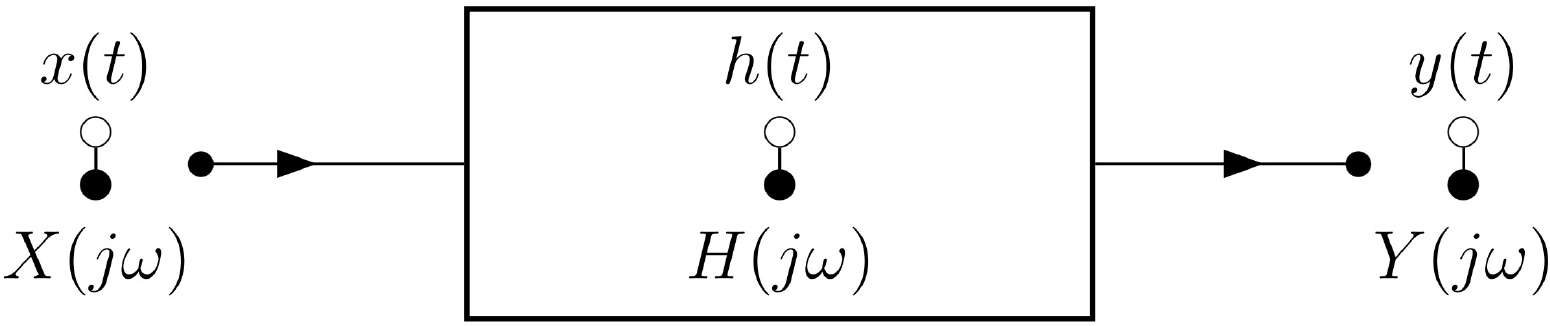
\includegraphics[width=0.6\columnwidth]{images/frequenzgang_impulsantwort.png}
\end{center}

Die Impulsantwort $h(t)$ und die Übertragungsfunktion $H(s)$ sind ein\\
 \textbf{Laplace}-Transformationspaar:
$$ \boxed{ h(t) \, \laplace \, H(s) } $$


Das Ausgangssignal berechnet sich als: 
$$ \boxed{ y(t) = h(t) * x(t) \, \laplace \, Y(s) = H(s) \cdot X(s) } $$


\subsubsection{Zusammenhang Impulsantwort \& Einheitssprungantwort}

\begin{tabular}{ll c c ll}
	$h(t)$ & Impulsantwort 	& 	& $g(t)$ & Einheitssprungantwort 
\end{tabular}

$$ \boxed{ h(t) =  \frac{\diff g(t)}{\diff t}  \quad \Leftrightarrow \quad g(t) = \int\limits_{-\infty}^t  h(\tau) \, \diff \tau }  $$
$$ \boxed{ H(s) = s \cdot G(s) \quad \Leftrightarrow \quad G(s) = \frac{1}{s} H(s) }  $$


\subsubsection{Zusammenhang Impulsantwort \& Kausalität LTI-System}

\fbox{\parbox{0.9\columnwidth}{
Damit ein LTI-System kausal ist, muss dessen Impulsantwort $h(t)$ für alle $t < 0$ gleich Null sein. 
} }


\subsection{Zusammenschalten von LTI-Systemen}

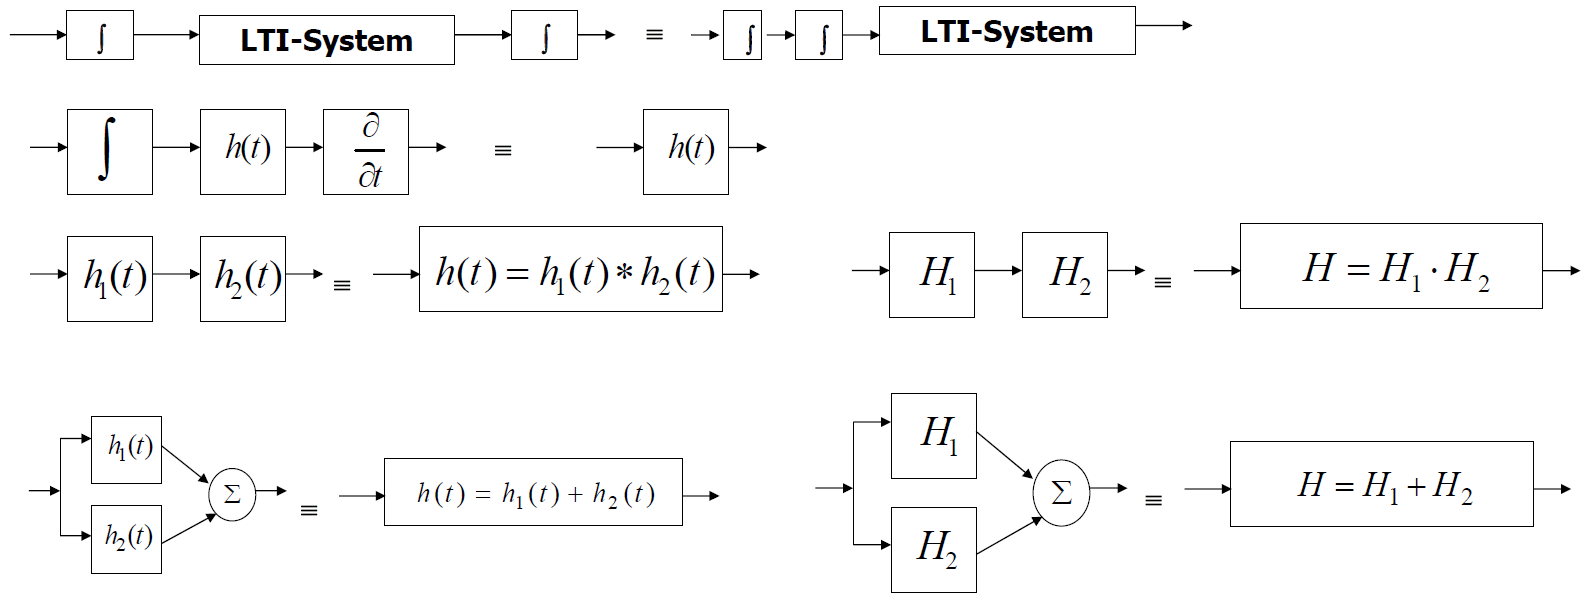
\includegraphics[width=\columnwidth]{images/zusammenschalten_von_LTI_systemen.png}


\subsection{Stabilität von LTI-Systemen}{177-181}

Bei den Betrachtungen von LTI-Systemen nehmen wir jeweils an, dass die Systeme \textbf{kausal} sind!


\subsubsection{BIBO-Stabilität}{177}

BIBO: \textbf{B}ounded \textbf{I}nput \textbf{B}ounded \textbf{O}utput

\vspace{0.2cm}

Ein LTI-System ist BIBO-stabil, wenn die \textbf{Impulsantwort absolut integrierbar} ist:

$$ \boxed{ \int\limits_{-\infty}^{\infty} |h(t)| \, \diff t < \infty } $$

\textrightarrow\ Für ein beschränktes Eingangssignal $x(t)$ ist auch das Ausgangssignal $y(t)$ beschränkt.


\subsubsection{Asymptotische Stabilität}{178}

Ein LTI-System ist asymptotisch stabil, wenn seine \textbf{Impulsantwort asymptotisch gegen Null} abklingt.

$$ \boxed{ \lim\limits_{t \to \infty} h(t) = 0 } $$

Alle kausalen LTI-Systeme mit \textbf{Polen nur in der linken $\bm{s}$-Halbebene} sind asymptotisch stabil! ($\sigma < 0$) \\
\textrightarrow\ Siehe Konvergenzhalbebene Abschnitt \ref{Konvergenzhalbebene}


\subsubsection{Instabilität}{178}

Ein LTI-System ist instabil, wenn: (ODER-Verknüpfung)

\vspace{0.1cm}

\begin{itemize}
	\item mindestens ein Pol der UTF in der \textbf{rechten $\bm{s}$-Halbebene} liegt ($\sigma > 0$) 
	\item mindestens ein \textbf{mehrfacher Pol auf der $\bm{\jimg \omega}$-Achse} der
		$s$-Ebene liegt (Pole müssen am gleichen Ort sein!) 
\end{itemize}


\subsubsection{Grenzstabilität}{178}

Ein LTI-System ist grenzstabil (quasistabil), wenn: (UND-Verknüpfung)

\vspace{0.1cm}

\begin{itemize}
	\item \textbf{kein} Pol in der rechten $s$-Halbebene liegt  ($\sigma \leq 0$)
	\item kein mehrfacher Pol auf der $\jimg \omega$-Achse der $s$-Ebene liegt
	\item auf der $\jimg \omega$-Achse mindestens ein \textbf{einfacher Pol} ist
\end{itemize}

\vspace{0.2cm}

\begin{minipage}[c]{0.6\columnwidth}
	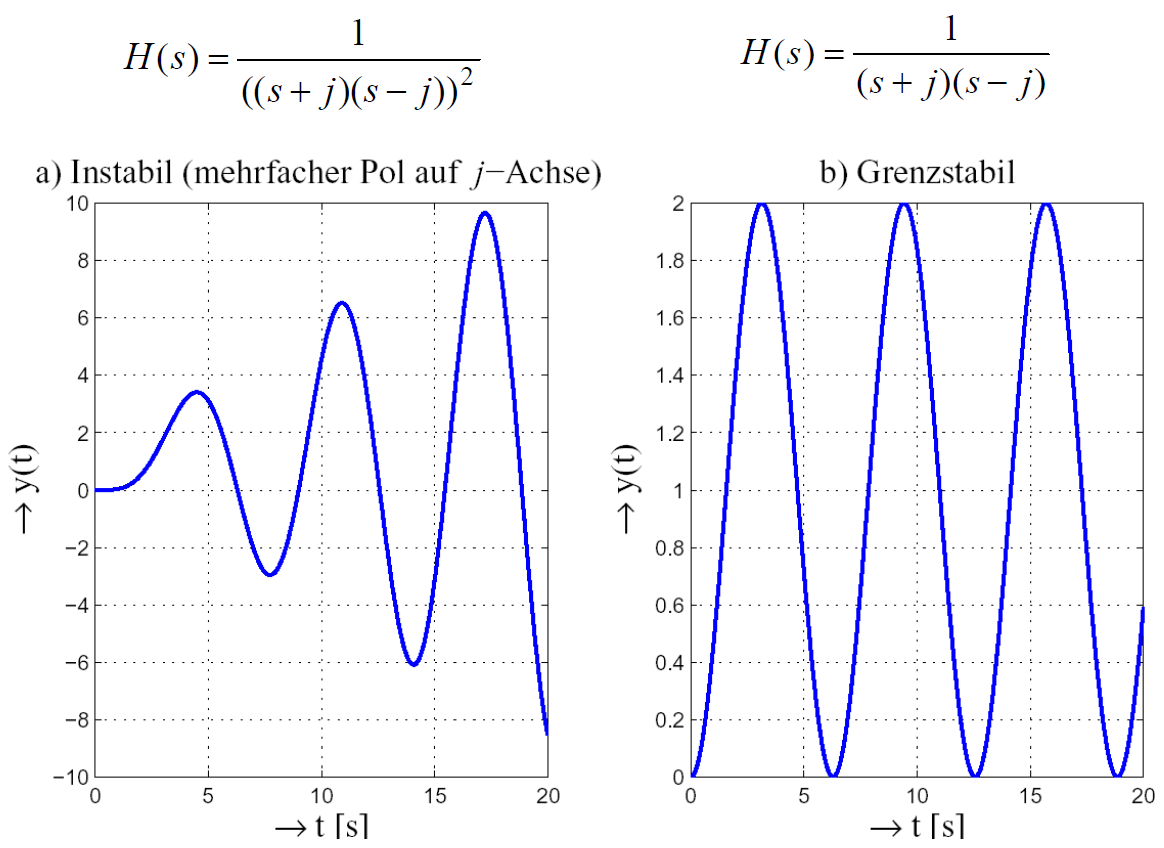
\includegraphics[width=\columnwidth]{images/grenzstabilitaet.png}
\end{minipage}
\hfill
\begin{minipage}[c]{0.38\columnwidth}
	\raggedright
	Ein System ist grenzstabil, wenn die Amplitude eines Signals 'erhalten' bleibt 
\end{minipage}


\subsubsection{Algebraische Stabilitätskriterien}{179-181}

\vspace{-0.2cm}
$$ P(s) = X(s) = a_n s^n + a_{n-1} s^{n-1} + ... + a_1 s + a_0 = a_n(s-p_1) \cdot ... \cdot (s-p_n) $$

Das Stabilitätskriterium betrachtet den \textbf{Nenner} $\boldsymbol{D(s)}$ der Übertragungsfunktion 
$$ H(s) = \frac{Y(s)}{X(s)} = \frac{N(s)}{D(s)}$$

\begin{itemize}
	\item Wenn der \textbf{Nenner} $\boldsymbol{D(s)}$ ein \textbf{Hurwitz-Polynom} ist, so ist das System \textbf{asymptotisch stabil.}
	\item Ein \textbf{modifiziertes Hurwitz-Polynom} ergibt ein \textbf{grenzstabiles System} \\
		\textrightarrow\ Polynom braucht \textbf{einfache Nullstellen} auf $\jimg \omega$-Achse
\end{itemize}

\vspace{0.3cm}

\myul{\textbf{Hurwitz-Kriterium}}

\vspace{0.1cm}

Ein Polynom $P(s)$ ist nur dann ein Hurwitz-Polynom wenn folgende \textbf{beiden} Bedingungen erfüllt sind: 

\vspace{0.1cm}

\begin{enumerate}
	\item Die Vorzeichen aller Koeffizienten $a_i$ von $P(s)$ sind \textbf{identisch} (und alle Koeffizienten $a_i$ sind vorhanden)
	\item Alle Hurwitz-Determinanten $D_1$ bis $D_n$ sind grösser als Null
\end{enumerate}

\vspace{0.3cm}

\myul{\textbf{Hurwitz-Determinanten}}

\begin{minipage}[c]{0.23\columnwidth}
	$$ D_1 = a_{n-1} > 0 $$
\end{minipage}
\hfill
\begin{minipage}[c]{0.27\columnwidth}
	$$ D_2 = 
	\begin{vmatrix}
		a_{n-1} & a_n \\
		a_{n-3} & a_{n-2} 
	\end{vmatrix}  > 0 $$
\end{minipage}
\hfill
\begin{minipage}[c]{0.45\columnwidth}
	$$ D_3 = \begin{vmatrix}
		a_{n-1} & a_n 		& 0			\\	
		a_{n-3} & a_{n-2} 	& a_{n-1} 	\\
		a_{n-5} & a_{n-4} 	& a_{n-3} 
	\end{vmatrix}  > 0 $$
\end{minipage}


\begin{minipage}[c]{0.6\columnwidth}
	$$ D_{n-1} = \begin{vmatrix}
		a_{n-1} & a_n 		& 0 		& 0 		& \cdots 	& 0 	\\
		a_{n-3} & a_{n-2} 	& a_{n-1} 	& a_n 		& 0 		& 0 	\\
		a_{n-5} & a_{n-4} 	& a_{n-3} 	& a_{n-2}	& \cdots 	& 0 	\\
		\vdots 	& \vdots  	& \vdots  	& \vdots  	& \ddots 	& 0 	\\
		0 		& 0 		& 0 		& \cdots 	& 0 		& a_1 
	\end{vmatrix}  > 0 $$
\end{minipage}
\hfill
\begin{minipage}[c]{0.38\columnwidth}
	$$ D_n = a_0 \, D_{n-1} > 0  $$
\end{minipage}


\subsection[Phasenlaufzeit]{Phasenlaufzeit $\tau_P(\omega)$}{183}

Die Phasenlaufzeit ist nur für \textbf{reine Sinus-Schwingungen} exakt bestimmbar! \\
Das System ist beschrieben durch:
$$ x(t) = A \cdot \sin(\omega_0 t + \gamma)$$
$$ H( \jimg \omega) = \alpha \cdot e^{- \jimg \omega t_0} \, \laplace \, h(t) = \alpha \cdot \delta(t - t_0) $$


Das Ausgangssignal $y(t) = x(t) * h(t)$ ist gegenüber dem Eingangssignal $x(t)$ mit $\alpha$ gewichtet und um die Zeit $t_0$ verzögert. \\
\textrightarrow\ \textbf{Diese Verzögerung wird Phasenlaufzeit genannt}

$$ \boxed{ \tau_P(\omega) = \frac{- \theta(\omega)}{\omega} } $$

$ \theta(\omega)$ entspricht dem Phasengang des Systems \textrightarrow\ Siehe Abschnitt \ref{Frequenzgang}


\example{Phasenlaufzeit}

\begin{center}
	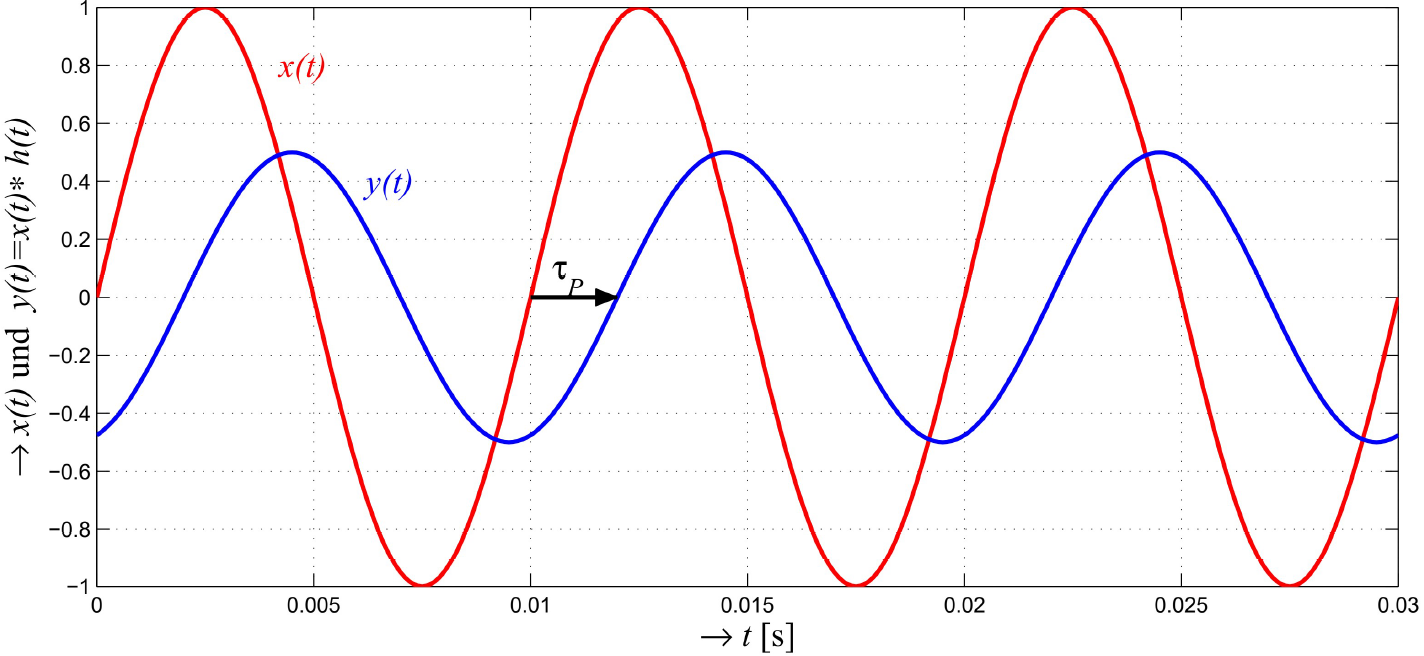
\includegraphics[width=0.8\columnwidth]{images/phasenlaufzeit.png}
\end{center}


\subsubsection{Negative Phasenlaufzeit}

Eine negative Phasenlaufzeit bedeutet \textbf{nicht}, dass ein System \textbf{akausal} ist!


\subsection[Gruppenlaufzeit]{Gruppenlaufzeit $\tau_G(\omega)$}

Definiert für Signale mit \textbf{mehreren Frequenzanteilen}

\vspace{0.2cm}

Bei amplitudenmodulierten Signalen bestimmt die Gruppenlaufzeit $\tau_G(\omega)$ die \textbf{Verzögerung der Hüllkurve} der AM.

$$ \boxed{ \tau_G(\omega) = \frac{- \diff \theta(\omega)}{\diff \omega} } $$

$ \theta(\omega)$ entspricht dem Phasengang des Systems \textrightarrow\ Siehe Abschnitt \ref{Frequenzgang}

\vspace{0.2cm}

Die Gruppenlaufzeit kann nur dann als \textbf{Laufzeit des Signals} interpretiert werden, wenn im Frequenzbereich des Signales die Gruppenlaufzeit und auch die Dämpfung ungefähr konstant sind.


\subsubsection{Negative Gruppenlaufzeit}

Bei \textbf{Vierpolen} mit \textbf{konzentrierten Elementen} ist in bestimmten Frequenzbereichen eine \textbf{negative Gruppenlaufzeit} 
möglich, insbesondere in Frequenzbereichen wo die Dämpfung stark ändert. (z.B. Nullstellen der UTF)

\vspace{0.2cm}

Bei negativer Gruppenlaufzeit erscheint die Wirkung \textbf{nicht} vor der Ursache! \\
\textrightarrow\ Das System ist \textbf{nicht} akausal! \\
Das Maximum der Hüllkurve kann am Ausgang kann aber \textbf{früher} als am Eingang auftreten.



\subsection{Phasenlaufzeit / Gruppenlaufzeit identisch}{186}

Die \textbf{Signalverzögernug, Phasenlaufzeit} $\bm{\tau_P(\omega)}$ und \textbf{Gruppenlaufzeit} $ \bm{\tau_G(\omega)}$ sind identisch, 
wenn
$$ \boxed{ \theta(\omega) = - \omega \cdot t_0  } $$

und der \textbf{Amplitudengang ebenfalls konstant} ist, d.h., $H(\jimg \omega) = \alpha \cdot e^{-\jimg \omega t_0}$ 

\vspace{0.2cm}

Die Signalverzögerung beträgt für \textbf{alle Frequenzen} $t_0 (= \tau_P = \tau_G) $ 




\subsection{Verzerrungen}{187-188}

Stimmt der zeitliche Verlauf einer Schwingung auf der Empfängerseite nicht mehr mit der Senderseite überein, arbeitet das 
Übertragungssystem \textbf{nicht verzerrungsfrei}.


\subsubsection{Lineare Verzerrung}

Ein \textbf{frequenzabhängiger Amplitudengang} $|H(\jimg \omega)| \neq$ const. oder ein \textbf{nichtlinearer Phasengang} (z.B. durch einen Tiefpassfilter) ergibt eine \textbf{lineare Verzerrung}. \\
Verzerrungsfrei: $|H(\jimg \omega)| = \alpha$ und $\theta(\omega) = -\omega t_0$.


\subsubsection{Nichtlineare Verzerrung}

Nichtlineare Verzerrungen werden durch \textbf{Übersteuerung} des Systems \textbf{(Kanal)} oder dessen \textbf{nichtlineare Kennlinie} 
hervorgerufen.

\vspace{0.1cm}

Durch nichtlineare Verzerrungen treten \textbf{neue}, im Ursprungssignal nicht enthaltene \textbf{Schwingungen} auf.

\vspace{0.1cm}

Ein \textbf{Mass} für nichtlineare Verzerrungen ist der \textbf{Klirrfaktor}.


\subsection{Klirrfaktor}{186}

Verhältnis des \textbf{Effektivwerts} der \textbf{neu} am Ausgang eines Systems entstandenen \textbf{Harmonischen} zum Effektivwert des 
gesamten Signals.

\vspace{0.2cm}

\begin{minipage}[c]{0.55\columnwidth}
	$$ \boxed{ k = \sqrt{\frac{U_2^2 + U_3^2 + ...+ U_n^2}{U_1^2 + U_2^2 + ...+ U_n^2}}} $$
\end{minipage}
\hfill
\begin{minipage}[c]{0.4\columnwidth}
	Es gilt: $1 > k \geq 0$
\end{minipage}

\vspace{0.2cm}

$U_1$ entspricht der Grundharmonischen!


\subsubsection{Klirrdämpfungsmass}

\vspace{-0.2cm}
$$ \boxed{ a_k = 20 \cdot \log_{10} \Big( \frac{1}{k}  \Big)  } $$


\subsubsection{Total Harmonic Distortion (THD)}

Wird vor allem im englisch-sprachigen Raum verwendet

\vspace{0.2cm}

\begin{minipage}[c]{0.55\columnwidth}
	$$ \boxed{  \text{THD} = \sqrt{\frac{U_2^2 + U_3^2 + ...+ U_n^2}{U_1^2} } } $$
\end{minipage}
\hfill
\begin{minipage}[c]{0.4\columnwidth}
	Es gilt: $\infty > \text{THD} \geq 0$
\end{minipage}

\vspace{0.2cm}

$U_1$ entspricht der Grundharmonischen! 

\vspace{0.2cm}
\begin{itemize}
	\item Für geringe Verzerrungen gilt: $\text{THD} \approx k$
	\item Im Allgemeinen gilt: $\text{THD} > k$
\end{itemize}


		\section{Anhang}


\subsection{Substitution bei Integralen}
% Von Zusammenfassung Analysis 2a

\begin{tabular}{ll}
    $\int \limits_0^{\sqrt{\pi}} x^3 \cdot \cos(x^2) \, \diff x$    & \cbl{Substitution: $a = x^2$ } \crd{ \textbf{auch auf Grenzen anwenden!}}                                                 \\
                                                                    & \cbl{$\diff a = 2 \, x \cdot \, \diff x$ \textrightarrow\ $\diff x = \frac{\diff a}{2x} = \frac{\diff a}{2 \sqrt{a}}$}
\end{tabular}

$\int \limits_{\crd{0}}^{\crd{\pi}} a \, \sqrt{a} \cdot \cos(a) \frac{\diff a}{2 \sqrt{a}} 
    = \int \limits_{\crd{0}}^{\crd{\pi}} a \, \sqrt{a} \cdot \cos(a) \, \frac{1}{2} \frac{1}{\sqrt{a}} \, \diff a
    = \frac{1}{2} \int \limits_{\crd{0}}^{\crd{\pi}} a \cdot \cos(a) \, \diff a = \ldots $


\subsubsection{Partielle Integration (Produktregel)}
\vspace{-1em}

\[\int_{a}^{b} f'\cdot g \, \diff x = \left[ f\cdot g \right]_{a}^{b} - \int_{a}^{b} f\cdot g' \, \diff x
\quad \text{oder} \quad
\int_{a}^{b} f\cdot g' \, \diff x = \left[ f\cdot g \right]_{a}^{b} - \int_{a}^{b} f' \cdot g \, \diff x
\]

Partielle Integration darf mehrfach angewendet werden. \\
\textbf{PI sollte wenn möglich vermieden werden! Produkte in Summen umschreiben!}\vspace{1em}

\textbf{LIATE} - Priorität für $g$ - funzione da derivare (non $\dots'$ nella forma base):


\subsection{Wichtige Integrale}

\begin{minipage}{0.48\columnwidth}
    $$ \frac{1}{T} \int\limits_{-T/2}^{T/2} \sin^2(\omega \, t) \,\diff t = \frac{1}{2} $$
\end{minipage}
\hfill
\begin{minipage}{0.48\columnwidth}
    $$ \frac{1}{T} \int\limits_{-T/2}^{T/2} \cos^2(\omega \, t) \, \diff t = \frac{1}{2} $$
\end{minipage}


\subsection{Trigonometrie}


% von Integraltransformationen Zusammenfassung	 
% \includegraphics[width=\columnwidth]{images/trigo.png} 

\begingroup
\renewcommand{\arraystretch}{2}
\setlength{\tabcolsep}{0mm}
\scalebox{0.33}{
\Huge
\begin{tabularx}{3\columnwidth}{rp{1mm}V{3}*{17}{C}}
    \rowcolor{subsectioncolor!30}$\bm{\alpha}$\phantom{${}^{\circ}$} && $0$ & $\dfrac{\pi}{6\mathstrut}$ & $\dfrac{\pi}{4}$ & $\dfrac{\pi}{3}$ & $\dfrac{\pi}{2}$ & $\dfrac{2\pi}{3}$ & $\dfrac{3\pi}{4}$ & $\dfrac{5\pi}{6}$ & $\pi$ & $\dfrac{7\pi}{6}$ & $\dfrac{5\pi}{4}$ & $\dfrac{4\pi}{3}$ & $\dfrac{3\pi}{2}$ & $\dfrac{5\pi}{3}$ & $\dfrac{7\pi}{4}$ & $\dfrac{11\pi}{6}$ & $2\pi$ \\\hline
    \rowcolor{subsectioncolor!30}$\bm{\alpha^\circ}$ && \phantom{${}^\circ$}$0^\circ$ & $30^\circ$ & $45^\circ$ & $60^\circ$ & $90^\circ$ & $120^\circ$ & $135^\circ$ & $150^\circ$ & $180^\circ$ & $210^\circ$ & $225^\circ$ & $240^\circ$ & $270^\circ$ & $300^\circ$ & $315^\circ$ & $330^\circ$ & $360^\circ$ \\\hline
    $\bm{\sin(\alpha)}$ && $0$ & $\dfrac{1}{2\mathstrut}$ & $\dfrac{\sqrt{2}}{2}$ & $\dfrac{\sqrt{3}}{2}$ & $1$ & $\dfrac{\sqrt{3}}{2}$ & $\dfrac{\sqrt{2}}{2}$ & $\dfrac{1}{2}$ & $0$ & $-\dfrac{1}{2}$ & $-\dfrac{\sqrt{2}}{2}$ & $-\dfrac{\sqrt{3}}{2}$ & $-1$ & $-\dfrac{\sqrt{3}}{2}$ & $-\dfrac{\sqrt{2}}{2}$ & $-\dfrac{1}{2}$ & $0$ \\\hline
    $\bm{\cos(\alpha)}$ && $1$ & $\dfrac{\sqrt{3}}{2\mathstrut}$ & $\dfrac{\sqrt{2}}{2}$ & $\dfrac{1}{2}$ & $0$ & $-\dfrac{1}{2}$ & $-\dfrac{\sqrt{2}}{2}$ & $-\dfrac{\sqrt{3}}{2}$ & $-1$ & $-\dfrac{\sqrt{3}}{2}$ & $-\dfrac{\sqrt{2}}{2}$ & $-\dfrac{1}{2}$ & $0$ & $\dfrac{1}{2}$ & $\dfrac{\sqrt{2}}{2}$ & $\dfrac{\sqrt{3}}{2}$ & $1$ \\\hline
    $\bm{\tan(\alpha)}$ && $0$ & $\dfrac{\sqrt{3}}{3\mathstrut}$ & $1$ & $\sqrt{3}$ & $\pm\infty$ & $-\sqrt{3}$ & $-1$ & $-\dfrac{\sqrt{3}}{3}$ & $0$ & $\dfrac{\sqrt{3}}{3}$ & $1$ & $\sqrt{3}$ & $\pm\infty$ & $-\sqrt{3}$ & $-1$ & $-\dfrac{\sqrt{3}}{3}$ & $0$ \\\hline
    $\bm{\cot(\alpha)}$ && $\pm\infty$ & $\sqrt{3}$ & $1$ & $\dfrac{\sqrt{3}}{3\mathstrut}$ & $0$ & $-\dfrac{\sqrt{3}}{3}$ & $-1$ & $-\sqrt{3}$ & $\pm\infty$ & $\sqrt{3}$ & $1$ & $\dfrac{\sqrt{3}}{3}$ & $0$ & $-\dfrac{\sqrt{3}}{3}$ & $-1$ & $-\sqrt{3}$ & $\pm\infty$ \\
\end{tabularx}}
\endgroup


\subsubsection{Komplexe Darstellung}

\begin{minipage}{0.48\columnwidth}
    $$ \sin(x) = \frac{e^{\jimg x} - e^{-\jimg x}}{2 \jimg} $$ 
\end{minipage}	
\hfill
\begin{minipage}{0.48\columnwidth}
    $$ \cos(x) = \frac{e^{\jimg x} + e^{- \jimg x}}{2} $$ 
\end{minipage}		


\subsubsection{Beziehungen zwischen $\bm{\sin(x)}$ und $\bm{\cos(x)}$}\label{chap:trigo-beziehungen}

\renewcommand{\arraystretch}{1.2}
\begin{tabular}{ll}
    $\sin(-a) = -\sin(a)$                                                               & $\cos(-a) = \cos(a)$          \\
    $\sin(\pi - a) = \sin(a)$                                                           & $\cos(\pi -a) = - \cos(a)$    \\		
    $\sin(\pi + a) = -\sin(a)$                                                          & $\cos(\pi + a) = - \cos(a)$   \\	
    $\sin \Big( \frac{\pi}{2} - a \Big) = \sin \Big( \frac{\pi}{2} + a \Big) = \cos(a)$ & $\cos \Big( \frac{\pi}{2} - a \Big) = - \cos \Big( \frac{\pi}{2} + a \Big) = \sin(a)$\\
    $\sin \Big( a - \frac{\pi}{2} \Big) = -\cos(a)$                                     & $\cos \Big( a - \frac{\pi}{2} \Big) = \sin(a)$ \\
    $\tan(-\alpha) = -\tan(\alpha)$ & \cor{$\arctan$ restituisce solo angoli $\in [-\pi, \pi]$!}
\end{tabular}


\subsubsection{Additionstheoreme}

\begin{tabular}{ll}
    $\sin(a \pm b) = \sin(a) \cdot \cos(b) \pm \cos(a) \cdot \sin(b)$   & $\tan(a \pm b) = \frac{\tan(a) \pm \tan(b)}{1 \mp \tan(a) \cdot \tan(b)}$        \\
    $\cos(a \pm b) = \cos(a) \cdot \cos(b) \mp \sin(a) \cdot \sin(b) $  & 
\end{tabular}


\subsubsection{Summen und Differenzen}

\begin{tabular}{ll}
    $\sin(a) + \sin(b) = 2 \cdot \sin \Big( \frac{a+b}{2} \Big) \cdot \cos \Big( \frac{a-b}{2} \Big)$   \\
    $\sin(a) - \sin(b) = 2 \cdot \sin \Big( \frac{a-b}{2} \Big) \cdot \cos \Big( \frac{a+b}{2} \Big)$   \\
    $\cos(a) + \cos(b) = 2 \cdot \cos \Big( \frac{a+b}{2} \Big) \cdot \cos \Big( \frac{a-b}{2} \Big)$   \\
    $\cos(a) - \cos(b) = -2 \cdot \sin \Big( \frac{a+b}{2} \Big) \cdot \sin \Big( \frac{a-b}{2} \Big)$  \\
    $\tan(a) \pm \tan(b) = \frac{\sin(a \pm b)}{\cos(a) \cdot \cos(b)}$ 
\end{tabular}


\subsubsection{Produkte}

\begin{tabular}{l}
    $\sin(a) \cdot \sin(b) = \frac{1}{2} \big( \cos(a-b) - \cos(a+b) \big) $ \\
    $\cos(a) \cdot \cos(b) = \frac{1}{2} \big( \cos(a-b) + \cos(a+b) \big) $ \\	
    $\sin(a) \cdot \cos(b) = \frac{1}{2} \big( \sin(a-b) + \sin(a+b) \big) $ \\
    $\cos(a) \cdot \sin(b) = \frac{1}{2} \left( \sin(b - a) + \sin(b + a) \right)$
\end{tabular}


\subsubsection{Winkelvielfache und Halbwinkel}

\begin{tabular}{ll}
    $\sin(2a) = 2 \, \sin(a) \cdot \cos(a)$                                 & $\cos(2a) = \cos^2(a) - \sin^2(a)$ \\
    $\sin(3a) = 3 \, \sin(a) -4 \, \sin^3(a)$                               & $\cos(3a) = 4 \, \cos^3(a) -3 \, \cos(a)$\\ \medskip
    $\sin(4a) = 8 \, \cos^3(a) \sin(a) - 4 \, \cos(a) \sin(a)$              & $\cos(4a) = 8 \, \cos^4(a) - 8 \, \cos^2(a) + 1$\\
    $\sin \Big( \frac{a}{2} \Big) = \sqrt{\frac{1}{2} \big(1-\cos(a) \big)}$& $\cos \Big( \frac{a}{2} \Big) = \sqrt{\frac{1}{2} \big(1+\cos(a) \big)}$
\end{tabular}


\subsubsection{Potenzen}

\begin{tabular}{ll}
    $\sin^2(a) = \frac{1}{2} \big(1-\cos(2a) \big)$                   & $\cos^2(a) = \frac{1}{2} \big(1+\cos(2a) \big)$                     \\	
    $\sin^3(a) = \frac{1}{4} \big(3\, \sin(a) - \sin(3a) \big)$       & $\cos^3(a) = \frac{1}{4} \big(\cos(3a) + 3 \, \cos(a) \big)$        \\	
    $\sin^4(a) = \frac{1}{8} \big(\cos(4a) -4 \, \cos(2a) +3 \big)$   & $\cos^4(a) = \frac{1}{8} \big(\cos(4a) + 4 \, \cos(2a) +3 \big)$
\end{tabular}


\subsection{Zusammenhang Harmonische -- Oberwellen}

\begin{center}
    \begin{tabular}{lll}
        \toprule
        \textbf{Kreisfrequenz}  & \textbf{Harmonische}      & \textbf{Oberwellen}   \\
        \midrule
        $\omega_0$              & 1. Harmonische            & Grundwelle            \\
        \midrule
        $2 \cdot \omega_0$      & 2. Harmonische            & 1. Oberwelle          \\
        \midrule
        $3 \cdot \omega_0$      & 3. Harmonische            & 2. Oberwelle          \\
        \midrule
        \vdots                  & \vdots                    & \vdots                \\
        \midrule
        $n \cdot \omega_0$      & $n$. Harmonische          & $(n-1)$. Oberwelle    \\
        \bottomrule
    \end{tabular}
\end{center}


\subsection{Fourier-Transformation: Wichtige Korrespondenzpaare}

\begin{center}
    \begin{tabular}{l c l}
        \toprule
        \textbf{Zeitbereich}    &               & \textbf{Frequenzbereich}                                                  \\
        \midrule
        Rechteck                & $\laplace$    & $\mathrm{sinc}(a \, \omega)$ \textrightarrow\ Support von $-a \ldots a$   \\
        \midrule
        Dirac-Rechen            & $\laplace$    & Dirac-Rechen mit grösserem Abstand                                        \\
        \midrule
        $\delta(t)$             & $\laplace$    & $1$                                                                       \\
        \midrule
        $\cos(\omega_0 \, t)$   & $\laplace$    & $\pi(\delta( \omega + \omega_0) + \delta ( \omega - \omega_0))$           \\
        \midrule
        $ \sin(\omega_0 \, t)$  & $\laplace$    & $\jimg \pi(\delta( \omega + \omega_0) - \delta ( \omega - \omega_0))$     \\
        \bottomrule
    \end{tabular}
\end{center}


\subsection{Laplace-Transformation: Wichtige Korrespondenzpaare}

% Gemäss Modul Integraltransformationen
\vspace{-0.2cm}
$$ u(t) = \text{Einheitssprung} $$

\begin{center}
    \begin{tabular}{l c l}
        \toprule
        \textbf{Zeitbereich}            &               & \textbf{Frequenzbereich}          \\
        \midrule
        $u(t)$                          & $\laplace$    & $ \frac{1}{s}$                    \\
        \midrule        
        $u(t) \cdot t^n $               & $\laplace$    & $\frac{n!}{s^{n+1}}$              \\
        \midrule
        $u(t) \cdot e^{a \,t} $         & $\laplace$    & $\frac{1}{s-a}$                   \\
        \midrule
        $u(t) \cdot \cos(\omega \, t) $ & $\laplace$    & $\frac{s}{s^2 + \omega^2}$        \\
        \midrule
        $u(t) \cdot \sin(\omega \, t )$ & $\laplace$    & $\frac{\omega}{s^2 + \omega^2}$   \\
        \midrule
        $\delta(t)$                     & $\laplace$    & $1(s)$                            \\
        \bottomrule
    \end{tabular}
\end{center}


\subsection{Zusammenstellung einiger Dichtefunktionen}
\label{Zusammenstellung einiger Dichtefunktionen}

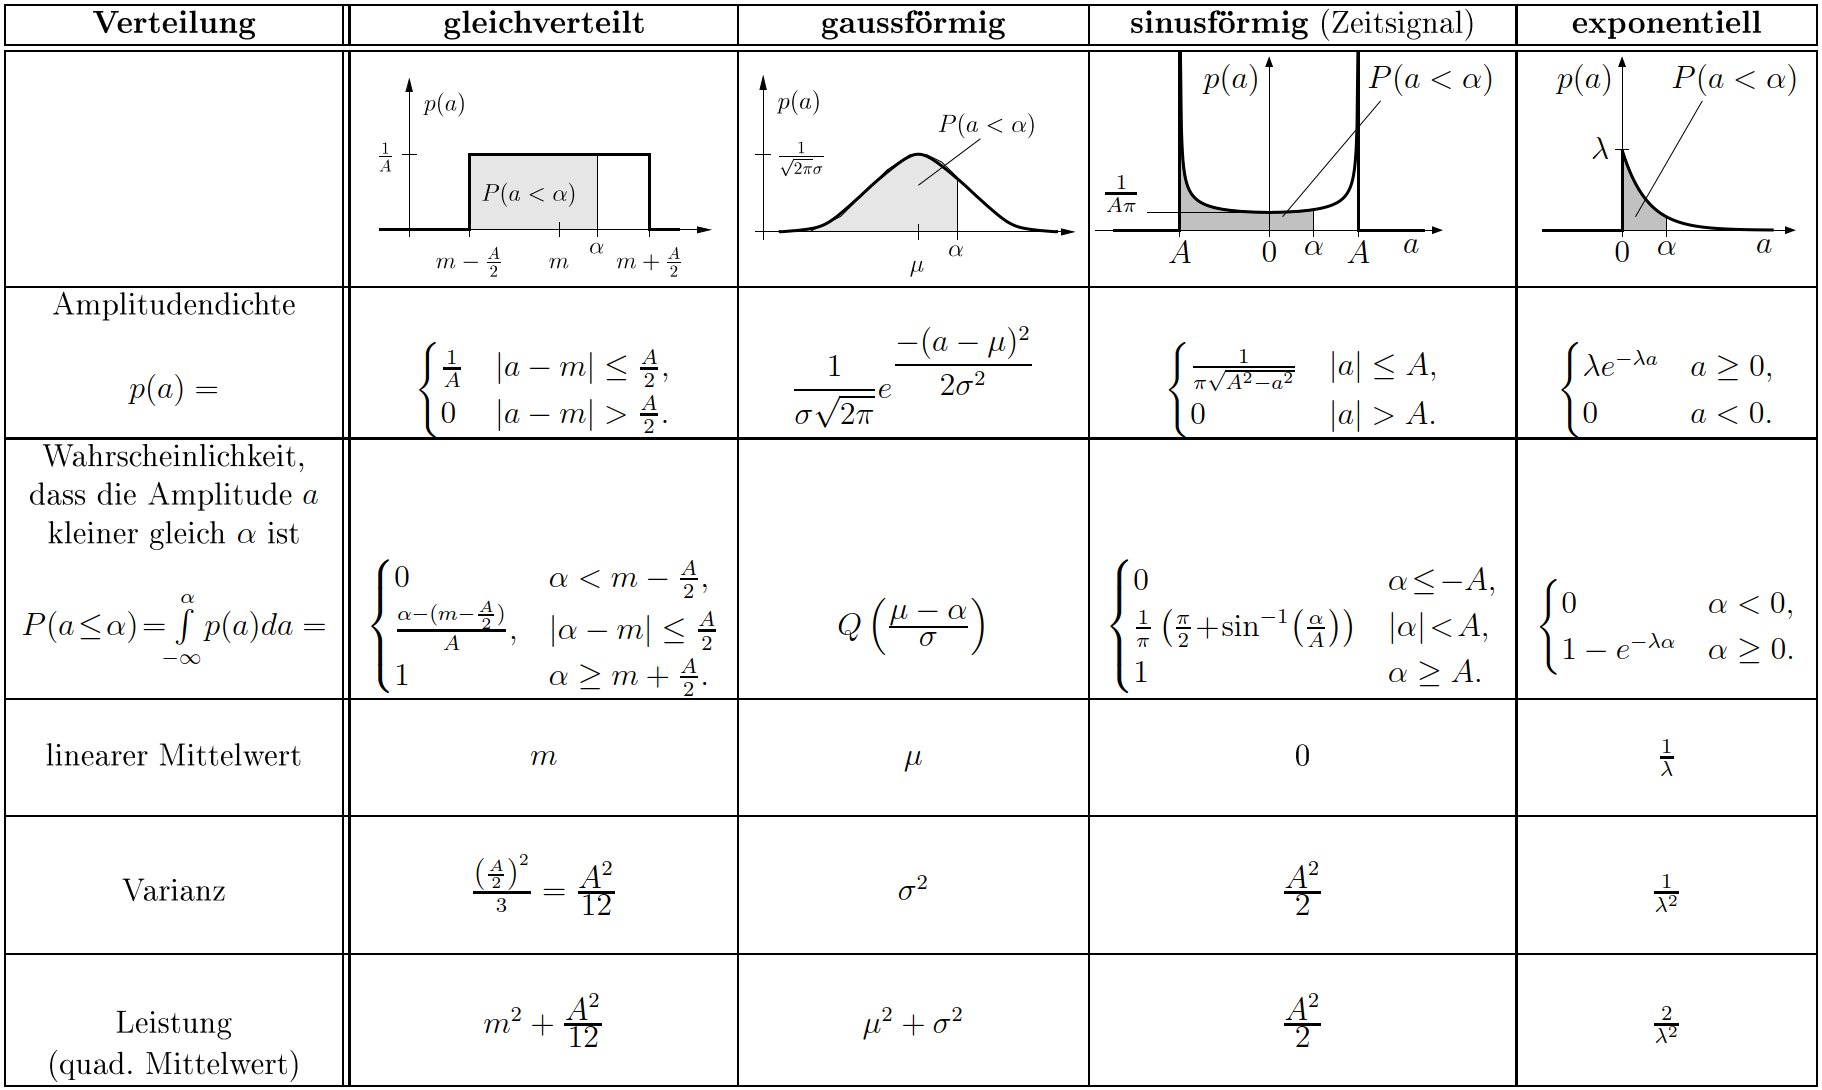
\includegraphics[width=\columnwidth]{images/zusammenstellung_dichtefunktionen.png}


\subsection{Zusammenstellung einiger Signale und ihrer Funktionen}

\resizebox{\columnwidth}{!}{
\begin{tabular}{|l||c|c|c|}
        \hline
        \multirow{2}{*}{\huge \textbf{Signal / Funktion}} & \multicolumn{2}{c|}{Endliche Signalleistung $0 < P_n < \infty, (W_n = \infty)$} & Endliche Signalenergie $W_n < \infty$ \\
        \cline{2-4}
        & periodisch ($\omega_0 = 2\pi/T_0$) & stochastisch (stationär) & abklingend, zeitbegrenzt \\
        \hline\hline
        
        Autokorrelationsfunktion (AKF) & 
        $\displaystyle \varphi(\tau) = \frac{1}{T_0} \int\limits_{-T_0/2}^{T_0/2} f(t)f(t+\tau)dt$ & 
        $\displaystyle \varphi(\tau) = \lim_{T\to\infty} \frac{1}{T} \int\limits_{-T/2}^{T/2} f(t)f(t+\tau)dt$ & 
        $\displaystyle \varphi(\tau) = \int\limits_{-\infty}^{\infty} f(t)f(t+\tau)dt$ \\
        \hline
        
        Fourier-Transformation der AKF & 
        $\displaystyle P_n = \frac{1}{T_0} \int\limits_{-T_0/2}^{T_0/2} \varphi(\tau)e^{-jn\omega_0\tau}d\tau$ & 
        $\displaystyle \Phi(j\omega) = \int\limits_{-\infty}^{\infty} \varphi(\tau)e^{-j\omega\tau}d\tau$ & 
        $\displaystyle E(j\omega) = \int\limits_{-\infty}^{\infty} \varphi(\tau)e^{-j\omega\tau}d\tau$ \\
        \hline
        
        Rücktransformation der AKF & 
        $\displaystyle \varphi(\tau) = \sum_{n=-\infty}^{\infty} P_n e^{jn\omega_0\tau}$ & 
        $\displaystyle \varphi(\tau) = \frac{1}{2\pi} \int\limits_{-\infty}^{\infty} \Phi(j\omega)e^{j\omega\tau}d\omega$ & 
        $\displaystyle \varphi(\tau) = \frac{1}{2\pi} \int\limits_{-\infty}^{\infty} E(j\omega)e^{j\omega\tau}d\omega$ \\
        \hline
        
        Amplitudenspektrum & 
        $\displaystyle c_n = \frac{1}{T_0} \int\limits_{-T_0/2}^{T_0/2} f(t)e^{-jn\omega_0 t}dt$ & 
        -- & 
        -- \\
        \hline
        
        Amplitudendichtespektrum & 
        -- & 
        -- & 
        $\displaystyle F(j\omega) = \int\limits_{-\infty}^{\infty} f(t)e^{-j\omega t}dt$ \\
        \hline
        
        Leistungsspektrum & 
        $\displaystyle P_n = |c_n|^2$ & 
        -- & 
        -- \\
        \hline
        
        Leistungsdichtespektrum & 
        -- & 
        $\displaystyle \Phi(j\omega) = E \left\{ \lim_{T \to \infty} \frac{1}{T} \left| \int\limits_{-T/2}^{T/2} f(t)e^{-j\omega t}dt \right|^2 \right\}$ & 
        -- \\
        \hline
        
        Energiedichtespektrum & 
        -- & 
        -- & 
        $\displaystyle E(j\omega) = |F(j\omega)|^2$ \\
        \hline
        
        Energie & 
        -- & 
        -- & 
        $\displaystyle W = \varphi(0) = \frac{1}{2\pi} \int\limits_{-\infty}^{\infty} E(j\omega)d\omega$ \\
        \hline
        
        Leistung & 
        $\displaystyle P = \varphi(0) = \sum_{n=-\infty}^{\infty} P_n$ & 
        $\displaystyle P = \varphi(0) = \frac{1}{2\pi} \int\limits_{-\infty}^{\infty} \Phi(j\omega)d\omega$ & 
        -- \\
        \hline
        
        Fourier-Reihe & 
        $\displaystyle f(t) = \sum_{n=-\infty}^{\infty} c_n e^{jn\omega_0 t}$ & 
        -- & 
        -- \\
        \hline
        
        Fourier-Integral & 
        -- & 
        -- & 
        $\displaystyle f(t) = \frac{1}{2\pi} \int\limits_{-\infty}^{\infty} F(j\omega)e^{j\omega t}d\omega$ \\
        \hline
    \end{tabular}}

\subsection{Beispiele -- Amplitudendichten}
\label{Beispiele - Amplitudendichte}

\subsubsection{Sinus}

\begin{minipage}[c]{0.48\columnwidth}
    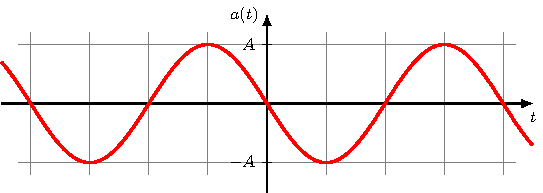
\includegraphics[width=\columnwidth]{images/PDF/sinussignal.pdf} 
\end{minipage}
\hfill
\begin{minipage}[c]{0.48\columnwidth}
    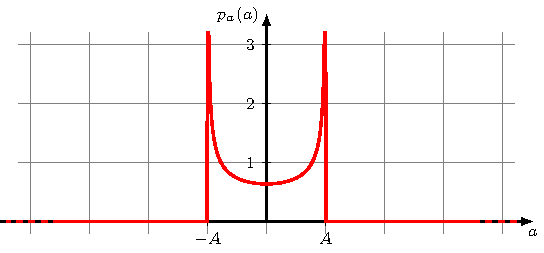
\includegraphics[width=\columnwidth]{images/PDF/sinussignal_amplitudendichte.pdf} 
\end{minipage}


\subsubsection{Dreieck}

\begin{minipage}[c]{0.48\columnwidth}
    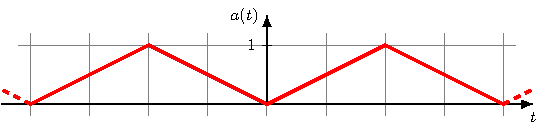
\includegraphics[width=\columnwidth]{images/PDF/dreiecksignal.pdf} 
\end{minipage}
\hfill
\begin{minipage}[c]{0.48\columnwidth}
    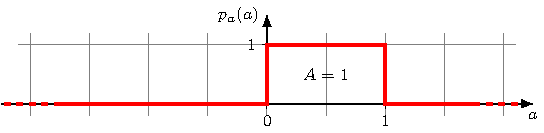
\includegraphics[width=\columnwidth]{images/PDF/dreiecksignal_amplitudendichte.pdf} 
\end{minipage}


\subsubsection{Rechteck}
\label{Rechteck} 

\begin{minipage}[c]{0.48\columnwidth}
    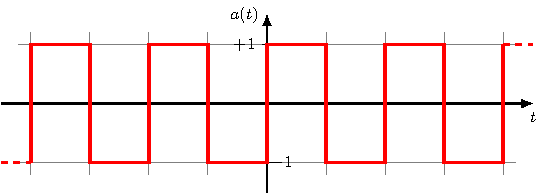
\includegraphics[width=\columnwidth]{images/PDF/rechtecksignal.pdf} 
\end{minipage}
\hfill
\begin{minipage}[c]{0.48\columnwidth}
    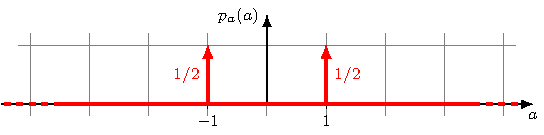
\includegraphics[width=\columnwidth]{images/PDF/rechtecksignal_amplitudendichte.pdf} 
\end{minipage}


    \end{layout}
\end{document}
